% Options for packages loaded elsewhere
\PassOptionsToPackage{unicode}{hyperref}
\PassOptionsToPackage{hyphens}{url}
\PassOptionsToPackage{dvipsnames,svgnames,x11names}{xcolor}
%
\documentclass[
  letterpaper,
  DIV=11,
  numbers=noendperiod]{scrreprt}

\usepackage{amsmath,amssymb}
\usepackage{iftex}
\ifPDFTeX
  \usepackage[T1]{fontenc}
  \usepackage[utf8]{inputenc}
  \usepackage{textcomp} % provide euro and other symbols
\else % if luatex or xetex
  \usepackage{unicode-math}
  \defaultfontfeatures{Scale=MatchLowercase}
  \defaultfontfeatures[\rmfamily]{Ligatures=TeX,Scale=1}
\fi
\usepackage{lmodern}
\ifPDFTeX\else  
    % xetex/luatex font selection
\fi
% Use upquote if available, for straight quotes in verbatim environments
\IfFileExists{upquote.sty}{\usepackage{upquote}}{}
\IfFileExists{microtype.sty}{% use microtype if available
  \usepackage[]{microtype}
  \UseMicrotypeSet[protrusion]{basicmath} % disable protrusion for tt fonts
}{}
\makeatletter
\@ifundefined{KOMAClassName}{% if non-KOMA class
  \IfFileExists{parskip.sty}{%
    \usepackage{parskip}
  }{% else
    \setlength{\parindent}{0pt}
    \setlength{\parskip}{6pt plus 2pt minus 1pt}}
}{% if KOMA class
  \KOMAoptions{parskip=half}}
\makeatother
\usepackage{xcolor}
\usepackage{soul}
\setlength{\emergencystretch}{3em} % prevent overfull lines
\setcounter{secnumdepth}{5}
% Make \paragraph and \subparagraph free-standing
\ifx\paragraph\undefined\else
  \let\oldparagraph\paragraph
  \renewcommand{\paragraph}[1]{\oldparagraph{#1}\mbox{}}
\fi
\ifx\subparagraph\undefined\else
  \let\oldsubparagraph\subparagraph
  \renewcommand{\subparagraph}[1]{\oldsubparagraph{#1}\mbox{}}
\fi

\usepackage{color}
\usepackage{fancyvrb}
\newcommand{\VerbBar}{|}
\newcommand{\VERB}{\Verb[commandchars=\\\{\}]}
\DefineVerbatimEnvironment{Highlighting}{Verbatim}{commandchars=\\\{\}}
% Add ',fontsize=\small' for more characters per line
\usepackage{framed}
\definecolor{shadecolor}{RGB}{241,243,245}
\newenvironment{Shaded}{\begin{snugshade}}{\end{snugshade}}
\newcommand{\AlertTok}[1]{\textcolor[rgb]{0.68,0.00,0.00}{#1}}
\newcommand{\AnnotationTok}[1]{\textcolor[rgb]{0.37,0.37,0.37}{#1}}
\newcommand{\AttributeTok}[1]{\textcolor[rgb]{0.40,0.45,0.13}{#1}}
\newcommand{\BaseNTok}[1]{\textcolor[rgb]{0.68,0.00,0.00}{#1}}
\newcommand{\BuiltInTok}[1]{\textcolor[rgb]{0.00,0.23,0.31}{#1}}
\newcommand{\CharTok}[1]{\textcolor[rgb]{0.13,0.47,0.30}{#1}}
\newcommand{\CommentTok}[1]{\textcolor[rgb]{0.37,0.37,0.37}{#1}}
\newcommand{\CommentVarTok}[1]{\textcolor[rgb]{0.37,0.37,0.37}{\textit{#1}}}
\newcommand{\ConstantTok}[1]{\textcolor[rgb]{0.56,0.35,0.01}{#1}}
\newcommand{\ControlFlowTok}[1]{\textcolor[rgb]{0.00,0.23,0.31}{#1}}
\newcommand{\DataTypeTok}[1]{\textcolor[rgb]{0.68,0.00,0.00}{#1}}
\newcommand{\DecValTok}[1]{\textcolor[rgb]{0.68,0.00,0.00}{#1}}
\newcommand{\DocumentationTok}[1]{\textcolor[rgb]{0.37,0.37,0.37}{\textit{#1}}}
\newcommand{\ErrorTok}[1]{\textcolor[rgb]{0.68,0.00,0.00}{#1}}
\newcommand{\ExtensionTok}[1]{\textcolor[rgb]{0.00,0.23,0.31}{#1}}
\newcommand{\FloatTok}[1]{\textcolor[rgb]{0.68,0.00,0.00}{#1}}
\newcommand{\FunctionTok}[1]{\textcolor[rgb]{0.28,0.35,0.67}{#1}}
\newcommand{\ImportTok}[1]{\textcolor[rgb]{0.00,0.46,0.62}{#1}}
\newcommand{\InformationTok}[1]{\textcolor[rgb]{0.37,0.37,0.37}{#1}}
\newcommand{\KeywordTok}[1]{\textcolor[rgb]{0.00,0.23,0.31}{#1}}
\newcommand{\NormalTok}[1]{\textcolor[rgb]{0.00,0.23,0.31}{#1}}
\newcommand{\OperatorTok}[1]{\textcolor[rgb]{0.37,0.37,0.37}{#1}}
\newcommand{\OtherTok}[1]{\textcolor[rgb]{0.00,0.23,0.31}{#1}}
\newcommand{\PreprocessorTok}[1]{\textcolor[rgb]{0.68,0.00,0.00}{#1}}
\newcommand{\RegionMarkerTok}[1]{\textcolor[rgb]{0.00,0.23,0.31}{#1}}
\newcommand{\SpecialCharTok}[1]{\textcolor[rgb]{0.37,0.37,0.37}{#1}}
\newcommand{\SpecialStringTok}[1]{\textcolor[rgb]{0.13,0.47,0.30}{#1}}
\newcommand{\StringTok}[1]{\textcolor[rgb]{0.13,0.47,0.30}{#1}}
\newcommand{\VariableTok}[1]{\textcolor[rgb]{0.07,0.07,0.07}{#1}}
\newcommand{\VerbatimStringTok}[1]{\textcolor[rgb]{0.13,0.47,0.30}{#1}}
\newcommand{\WarningTok}[1]{\textcolor[rgb]{0.37,0.37,0.37}{\textit{#1}}}

\providecommand{\tightlist}{%
  \setlength{\itemsep}{0pt}\setlength{\parskip}{0pt}}\usepackage{longtable,booktabs,array}
\usepackage{calc} % for calculating minipage widths
% Correct order of tables after \paragraph or \subparagraph
\usepackage{etoolbox}
\makeatletter
\patchcmd\longtable{\par}{\if@noskipsec\mbox{}\fi\par}{}{}
\makeatother
% Allow footnotes in longtable head/foot
\IfFileExists{footnotehyper.sty}{\usepackage{footnotehyper}}{\usepackage{footnote}}
\makesavenoteenv{longtable}
\usepackage{graphicx}
\makeatletter
\def\maxwidth{\ifdim\Gin@nat@width>\linewidth\linewidth\else\Gin@nat@width\fi}
\def\maxheight{\ifdim\Gin@nat@height>\textheight\textheight\else\Gin@nat@height\fi}
\makeatother
% Scale images if necessary, so that they will not overflow the page
% margins by default, and it is still possible to overwrite the defaults
% using explicit options in \includegraphics[width, height, ...]{}
\setkeys{Gin}{width=\maxwidth,height=\maxheight,keepaspectratio}
% Set default figure placement to htbp
\makeatletter
\def\fps@figure{htbp}
\makeatother
\newlength{\cslhangindent}
\setlength{\cslhangindent}{1.5em}
\newlength{\csllabelwidth}
\setlength{\csllabelwidth}{3em}
\newlength{\cslentryspacingunit} % times entry-spacing
\setlength{\cslentryspacingunit}{\parskip}
\newenvironment{CSLReferences}[2] % #1 hanging-ident, #2 entry spacing
 {% don't indent paragraphs
  \setlength{\parindent}{0pt}
  % turn on hanging indent if param 1 is 1
  \ifodd #1
  \let\oldpar\par
  \def\par{\hangindent=\cslhangindent\oldpar}
  \fi
  % set entry spacing
  \setlength{\parskip}{#2\cslentryspacingunit}
 }%
 {}
\usepackage{calc}
\newcommand{\CSLBlock}[1]{#1\hfill\break}
\newcommand{\CSLLeftMargin}[1]{\parbox[t]{\csllabelwidth}{#1}}
\newcommand{\CSLRightInline}[1]{\parbox[t]{\linewidth - \csllabelwidth}{#1}\break}
\newcommand{\CSLIndent}[1]{\hspace{\cslhangindent}#1}

\KOMAoption{captions}{tableheading}
\makeatletter
\@ifpackageloaded{tcolorbox}{}{\usepackage[many]{tcolorbox}}
\@ifpackageloaded{fontawesome5}{}{\usepackage{fontawesome5}}
\definecolor{quarto-callout-color}{HTML}{909090}
\definecolor{quarto-callout-note-color}{HTML}{0758E5}
\definecolor{quarto-callout-important-color}{HTML}{CC1914}
\definecolor{quarto-callout-warning-color}{HTML}{EB9113}
\definecolor{quarto-callout-tip-color}{HTML}{00A047}
\definecolor{quarto-callout-caution-color}{HTML}{FC5300}
\definecolor{quarto-callout-color-frame}{HTML}{acacac}
\definecolor{quarto-callout-note-color-frame}{HTML}{4582ec}
\definecolor{quarto-callout-important-color-frame}{HTML}{d9534f}
\definecolor{quarto-callout-warning-color-frame}{HTML}{f0ad4e}
\definecolor{quarto-callout-tip-color-frame}{HTML}{02b875}
\definecolor{quarto-callout-caution-color-frame}{HTML}{fd7e14}
\makeatother
\makeatletter
\makeatother
\makeatletter
\@ifpackageloaded{bookmark}{}{\usepackage{bookmark}}
\makeatother
\makeatletter
\@ifpackageloaded{caption}{}{\usepackage{caption}}
\AtBeginDocument{%
\ifdefined\contentsname
  \renewcommand*\contentsname{Índice}
\else
  \newcommand\contentsname{Índice}
\fi
\ifdefined\listfigurename
  \renewcommand*\listfigurename{Lista de Figuras}
\else
  \newcommand\listfigurename{Lista de Figuras}
\fi
\ifdefined\listtablename
  \renewcommand*\listtablename{Lista de Tabelas}
\else
  \newcommand\listtablename{Lista de Tabelas}
\fi
\ifdefined\figurename
  \renewcommand*\figurename{Figura}
\else
  \newcommand\figurename{Figura}
\fi
\ifdefined\tablename
  \renewcommand*\tablename{Tabela}
\else
  \newcommand\tablename{Tabela}
\fi
}
\@ifpackageloaded{float}{}{\usepackage{float}}
\floatstyle{ruled}
\@ifundefined{c@chapter}{\newfloat{codelisting}{h}{lop}}{\newfloat{codelisting}{h}{lop}[chapter]}
\floatname{codelisting}{Listagem}
\newcommand*\listoflistings{\listof{codelisting}{Lista de Listagens}}
\makeatother
\makeatletter
\@ifpackageloaded{caption}{}{\usepackage{caption}}
\@ifpackageloaded{subcaption}{}{\usepackage{subcaption}}
\makeatother
\makeatletter
\@ifpackageloaded{tcolorbox}{}{\usepackage[skins, breakable]{tcolorbox}}
\makeatother
\makeatletter
\@ifundefined{shadecolor}{\definecolor{shadecolor}{rgb}{.97, .97, .97}}
\makeatother
\makeatletter
\makeatother
\ifLuaTeX
\usepackage[bidi=basic]{babel}
\else
\usepackage[bidi=default]{babel}
\fi
\babelprovide[main,import]{brazilian}
% get rid of language-specific shorthands (see #6817):
\let\LanguageShortHands\languageshorthands
\def\languageshorthands#1{}
\ifLuaTeX
  \usepackage{selnolig}  % disable illegal ligatures
\fi
\IfFileExists{bookmark.sty}{\usepackage{bookmark}}{\usepackage{hyperref}}
\IfFileExists{xurl.sty}{\usepackage{xurl}}{} % add URL line breaks if available
\urlstyle{same} % disable monospaced font for URLs
\hypersetup{
  pdftitle={Laboratório de Genética Molecular - Nupgen - DBC/Nupélia},
  pdflang={pt-BR},
  colorlinks=true,
  linkcolor={blue},
  filecolor={Maroon},
  citecolor={Blue},
  urlcolor={Blue},
  pdfcreator={LaTeX via pandoc}}

\title{Laboratório de Genética Molecular - Nupgen - DBC/Nupélia}
\author{}
\date{}

\begin{document}
\maketitle
\ifdefined\Shaded\renewenvironment{Shaded}{\begin{tcolorbox}[boxrule=0pt, borderline west={3pt}{0pt}{shadecolor}, sharp corners, interior hidden, frame hidden, breakable, enhanced]}{\end{tcolorbox}}\fi

\renewcommand*\contentsname{Índice}
{
\hypersetup{linkcolor=}
\setcounter{tocdepth}{2}
\tableofcontents
}
\bookmarksetup{startatroot}

\hypertarget{inuxedcio}{%
\chapter*{Início}\label{inuxedcio}}
\addcontentsline{toc}{chapter}{Início}

\markboth{Início}{Início}

Este é o manual online do \textbf{Nupgen}, o \textbf{Laboratório de
Genética Molecular do Nupélia (DBC/Nupélia)}. Aqui você poderá encontrar
textos explicativos sobre nossa linha de pesquisa, as metodologias
utilizadas em nosso laboratório, bem como os protocolos atualizados.
Este é um material introdutório destinado principalmente aos alunos do
laboratório e pode servir como guia para as tarefas mais técnicas.
Esperamos que ele funcione como um Procedimento Operacional Padrão (POP)
em nosso laboratório, mantendo as equipes alinhadas, elevando a
produtividade e evitando o desperdício de recursos dentro do
laboratório. Este manual não precisa ser lido de forma sequencial e cada
capítulo é independente de outros, no entanto, organizamos os capítulos
seguindo a lógica de trabalho no laboratório para tornar a leitura mais
fluida.

O objetivo deste manual não é substituir a colaboração entre alunos do
laboratório, mas sim garantir que pequenos detalhes não sejam perdidos
com o passar do tempo. Na verdade, esperamos que os tópicos deste manual
sejam exaustivamente discutidos entre os alunos, a fim de melhorar este
conteúdo e gerar novas perguntas que ajudem no desenvolvimento da
pesquisa.

Uma versão em PDF deste manual pode ser acessada pelo seguinte link:
\href{https://github.com/nupgen/book_nupgen/blob/master/_book/book-nupgen.pdf}{Manual
PDF}

Este manual foi escrito em \href{https://quarto.org/}{Quarto}.

A capa deste manual foi feita pelo Marco Paganini, do nosso laboratório.

\textbf{Organização: Bruno Mioto}

\textbf{Autores: Adrian Silva, Bárbara Scorsim, Bruno Mioto, Eloisa de
Páris, Laura Ramos e Mayara Passere}

\bookmarksetup{startatroot}

\hypertarget{genuxe9tica-molecular-e-marcadores}{%
\chapter{Genética Molecular e
Marcadores}\label{genuxe9tica-molecular-e-marcadores}}

\hypertarget{o-que-uxe9-a-genuxe9tica-molecular}{%
\section{O que é a genética
molecular?}\label{o-que-uxe9-a-genuxe9tica-molecular}}

A Genética Molecular utiliza o DNA como objeto de estudo. O DNA (ácido
desoxirribonucleico) é uma biomolécula capaz de armazenar a informação
biológica e perpetuá-la pelo processo de auto replicação
semiconservativa. Sua estrutura é uma dupla-fita helicoidal de
nucleotídeos, que por sua vez é composta por um grupo fosfato, uma
pentose e uma base nitrogenada. As duas fitas de DNA são unidas por meio
de ligações de hidrogênio entre as bases nitrogenadas. Existem quatro
bases nitrogenadas: Adenina (A), Timina (T), Citosina (C) e Guanina (G),
sendo a Adenina complementar à Timina, e a Citosina complementar à
Guanina. Portanto, uma fita de DNA consiste em uma sequência de
nucleotídeos, cuja ordem das bases nitrogenadas (A, T, C, G) determinam
as características biológicas. Embora as células possuam um aparato
enzimático complexo que garante uma alta fidelidade nas sequências
nucleotídicas durante a replicação do DNA, alguns ``erros de
replicação'' podem ser perpetuados. Esses ``erros'', além de fatores
ambientais (como a radiação, por exemplo), podem levar a mutações. As
mutações são a fonte do polimorfismo genético, que pode ser avaliado em
pesquisas na área da Biologia Molecular. Conhecer com profundidade os
mecanismos moleculares envolvidos na estrutura, replicação e geração de
polimorfismos é importante para compreensão o entendimento dos
protocolos e o domínio das análises feitas no laboratório, por isso,
recomenda-se a leitura de livros-base na área da Biologia Molecular e
Genética. Segue abaixo uma lista das principais referências na área:

\begin{itemize}
\item
  Bruce Alberts et al. (2017)
\item
  Anthony J. F. Griffiths et al. (2016)
\item
  Peter Snustad e Michael J. Simmons (2017)
\end{itemize}

\hypertarget{marcadores-moleculares}{%
\section{Marcadores Moleculares}\label{marcadores-moleculares}}

\bookmarksetup{startatroot}

\hypertarget{o-laboratuxf3rio}{%
\chapter{O Laboratório}\label{o-laboratuxf3rio}}

\hypertarget{apresentauxe7uxe3o-do-laboratuxf3rio}{%
\section{Apresentação do
Laboratório}\label{apresentauxe7uxe3o-do-laboratuxf3rio}}

O Nupgen é o \textbf{Laboratório de Genética Molecular do Nupélia}
(Núcleo de Pesquisas em Limnologia, Ictiologia e Aquicultura), da
\textbf{Universidade Estadual de Maringá} (UEM), Paraná, Brasil.
Coordenado pela Professora Dra. \textbf{Alessandra Valéria de Oliveira},
o Nupgen conta com pesquisadores, alunos de graduação e de
pós-graduação.

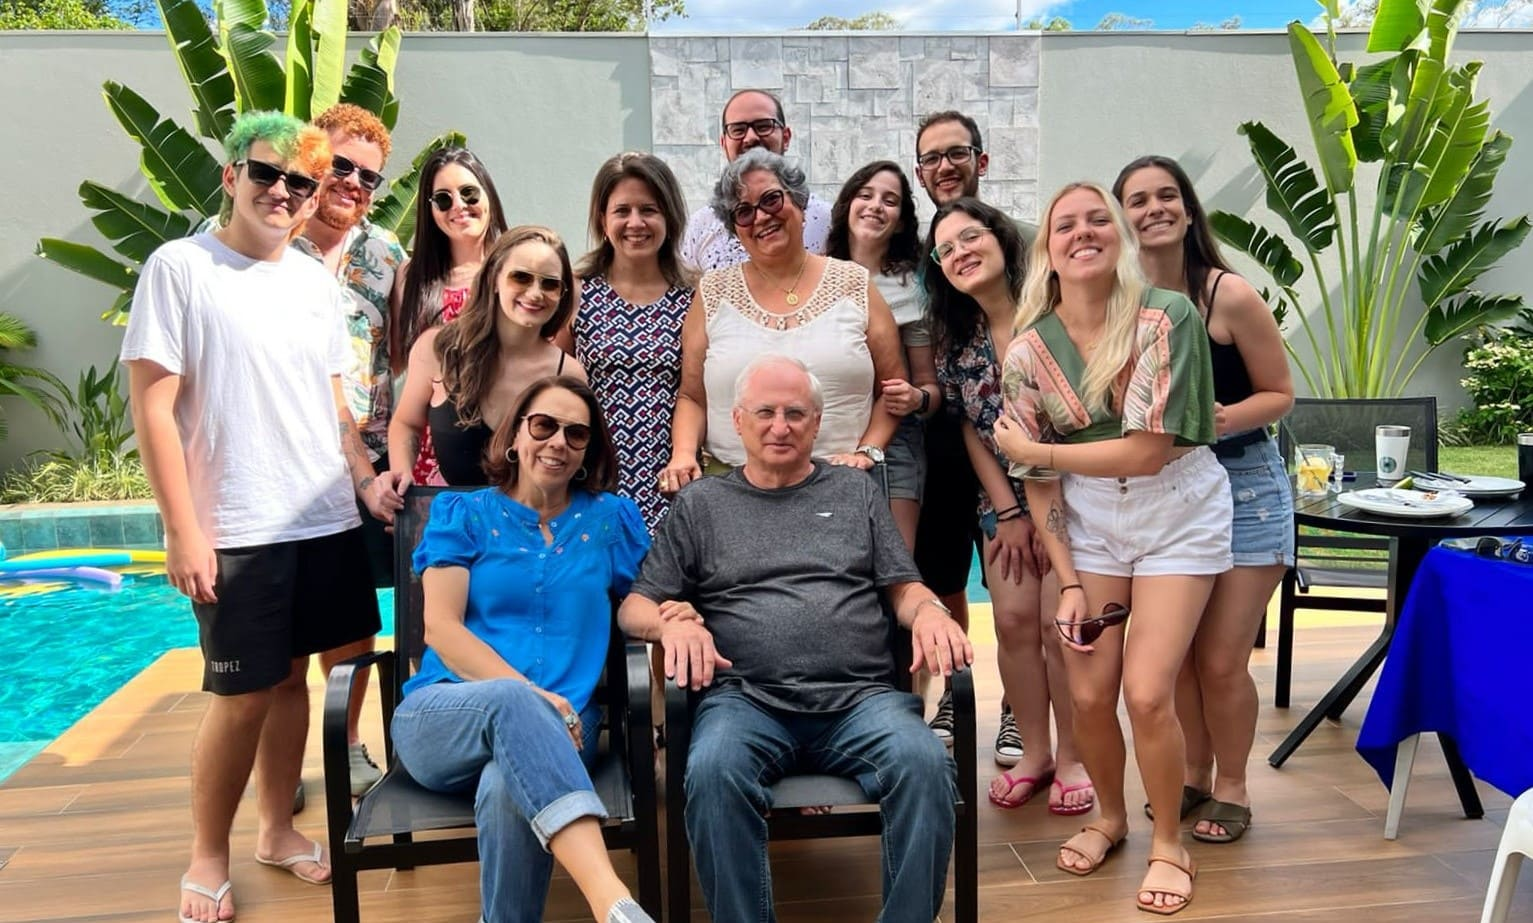
\includegraphics{figures/lab.jpeg}

\hypertarget{linhas-de-pesquisa}{%
\section{Linhas de Pesquisa}\label{linhas-de-pesquisa}}

Atualmente, o Nupgen realiza pesquisas objetivando detectar
polimorfismos genéticos em populações naturais de organismos: peixes,
parasitos, macrófitas, macroinvertebrados, microrganismos, além de
estudos utilizando DNA ambiental. Assim, os pesquisadores e alunos do
laboratório conduzem as seguintes linhas de pesquisa:

\hypertarget{taxonomia}{%
\subsection{Taxonomia}\label{taxonomia}}

Consiste na identificação dos organismos utilizando marcadores
moleculares. Projetos nessa linha de pesquisa costumam ocorrer em
parceria com outros laboratórios, que contribuem com a identificação
morfológica do organismo. A adição da genética molecular facilita a
detecção de espécies novas, híbridos e espécies crípticas, por exemplo.

\hypertarget{sistemuxe1tica-filogenuxe9tica}{%
\subsection{Sistemática
filogenética}\label{sistemuxe1tica-filogenuxe9tica}}

Diferente da taxonomia, projetos envolvendo Sistemática Filogenética não
buscam somente identificar os organismos, mas também levantar hipóteses
sobre a relação evolutiva entre eles (entre espécies de um mesmo gênero,
por exemplo).

\hypertarget{genuxe9tica-de-populauxe7uxf5es}{%
\subsection{Genética de
populações}\label{genuxe9tica-de-populauxe7uxf5es}}

A Genética de populações busca entender o fluxo gênico em uma população
natural, podendo endereçar questões acerca de processos de especiação e
adaptação, e podendo observar os efeitos da seleção natural, deriva
genética e dos efeitos de gargalo.

\hypertarget{biogeografia}{%
\subsection{Biogeografia}\label{biogeografia}}

Biogeografia é uma linha de pesquisa multidisciplinar que busca entender
a distribuição de um grupo de organismos em correlação com a evolução
ambiental (escala de tempo geológica), gerando resultados importantes
para a conservação da biodiversidade.

\hypertarget{organismos-estudados-no-nupgen}{%
\section{Organismos estudados no
Nupgen}\label{organismos-estudados-no-nupgen}}

\hypertarget{peixes}{%
\subsection{Peixes}\label{peixes}}

Ictiofaunas de ambientes aquáticos podem ser formadas por organismos
nativos e invasores. O estudo genético permite verificar níveis de
variação genética, perda de biodiversidade e alterações relacionadas a
processos dehibridização.

O estudo de populações nativas é importante para verificar a presença e
interação desses organismos de determinada região. Invasores, quando
presentes, modificam o habitat e o sistema onde foram introduzidos,
podendo levar a perda de biodiversidade local e alterações genéticas.
Assim, estudos moleculares permitem estimar a diversidade e verificar as
alterações genéticas que ocorrem nestes animais.

\hypertarget{macruxf3fitas}{%
\subsection{Macrófitas}\label{macruxf3fitas}}

As macrófitas aquáticas, quando invasoras, constituem uma ameaça em
termos ecológicos e também econômicos. A correta identificação e a
elucidação da diversidade genética desses organismos podem auxiliar na
compreensão dos mecanismos de dispersão e colonização, como também no
manejo adequado das espécies.

\hypertarget{parasitos}{%
\subsection{Parasitos}\label{parasitos}}

A relação parasito-hospedeiro possui grande importância nos ambientes
naturais. O conhecimento da biodiversidade de parasitos contribui com o
levantamento de espécies de hospedeiros no local, além de direcionar
métodos de manejo para parasitos com potencial zoonótico.

\hypertarget{microrganismos}{%
\subsection{Microrganismos}\label{microrganismos}}

Mesmo invisíveis a olho nu, os microrganismos possuem grande importância
em ambientes aquáticos, servindo como níveis inferiores na cadeia
alimentar. Alguns organismos podem influenciar na qualidade d'água, por
isso conhecer a diversidade destes microrganismos é fundamental.

\hypertarget{genes-opsins}{%
\subsection{Genes opsins}\label{genes-opsins}}

O estudo de proteínas visuais possibilita observar e comparar a
influência de fatores ecológicos no processo evolutivo de diversas
linhagens, identificando como as espécies se adaptam a diversas pressões
seletivas existentes no habitat.

\hypertarget{dna-ambiental}{%
\subsection{DNA Ambiental}\label{dna-ambiental}}

A partir de amostras ambientais, é possível obter fragmentos de DNA de
organismos que estiveram neste ambiente. Peixes, microrganismos,
anfíbios, parasitos e muitos outros organismos deixam rastros genéticos
e podemos estudá-los indiretamente a partir de técnicas de
sequenciamento de nova geração.

\bookmarksetup{startatroot}

\hypertarget{equipamentos}{%
\chapter{Equipamentos}\label{equipamentos}}

\hypertarget{centruxedfugas}{%
\section{Centrífugas}\label{centruxedfugas}}

A centrífuga é um aparelho que possui a finalidade de separar
substâncias que possuem densidades diferentes em uma mistura via
decantação. É utilizada em etapas da extração de DNA e durante o
processo de purificação das amostras. O tempo e a rotação por minuto
(rpm) podem ser ajustados de acordo com a necessidade do pesquisador. É
importante lembrar de sempre balancear os tubos dentro da centrífuga
antes da sua utilização, ou seja, dispor os tubos de uma forma que haja
o balanceamento dos pesos para não descalibrar o aparelho (ver quadro
Balanceamento da centrífuga). No Nupgen temos dois modelos de
centrífugas:

\hypertarget{centruxedfuga-mrc-scen-206-6000-rpm-confirmar-marcamodelo}{%
\subsection{Centrífuga MRC SCEN-206 6000 rpm *confirmar
marca/modelo*}\label{centruxedfuga-mrc-scen-206-6000-rpm-confirmar-marcamodelo}}

Nessa centrífuga cabem \textbf{18} microtubos de 1,5 mL. Não é
refrigerada.

\begin{figure}

{\centering 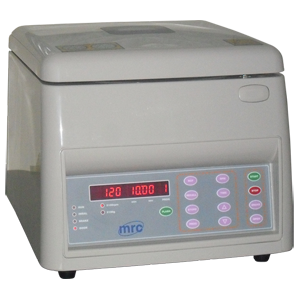
\includegraphics[width=\textwidth,height=3.125in]{figures/equipamentos/Centrifuga_MRC_SCEN-206.png}

}

\caption{Essa centrífuga encontra-se no laboratório do Bloco G80.}

\end{figure}

\hypertarget{centruxedfuga-eppendorf-5424}{%
\subsection{Centrífuga Eppendorf
5424}\label{centruxedfuga-eppendorf-5424}}

Nessa centrífuga cabem \textbf{24} microtubos de 1,5 mL. Não é
refrigerada.

\begin{figure}

{\centering 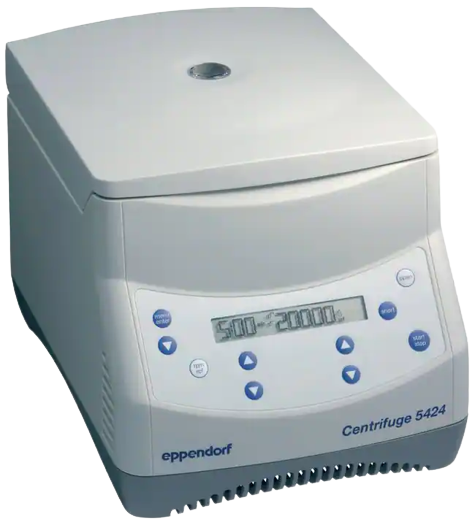
\includegraphics[width=\textwidth,height=3.125in]{figures/equipamentos/Centrifuga_Eppendorf_5424_2.png}

}

\caption{Essa centrífuga encontra-se no laboratório do Bloco G90.}

\end{figure}

\begin{tcolorbox}[enhanced jigsaw, colback=white, toprule=.15mm, rightrule=.15mm, opacityback=0, left=2mm, arc=.35mm, bottomrule=.15mm, breakable, leftrule=.75mm]
\begin{minipage}[t]{5.5mm}
\textcolor{quarto-callout-caution-color}{\faFire}
\end{minipage}%
\begin{minipage}[t]{\textwidth - 5.5mm}

\textbf{Balanceamento da centrífuga}\vspace{2mm}

É essencial que a centrífuga esteja balanceada com as amostras, ou então
ela pode danificar o eixo de rotação e quebrar.

Para isso, utilizamos os seguintes diagramas:

\hypertarget{balanceamento-da-centruxedfuga-de-18-amostras}{%
\subsection{Balanceamento da centrífuga de 18
amostras}\label{balanceamento-da-centruxedfuga-de-18-amostras}}

\begin{figure}[H]

{\centering 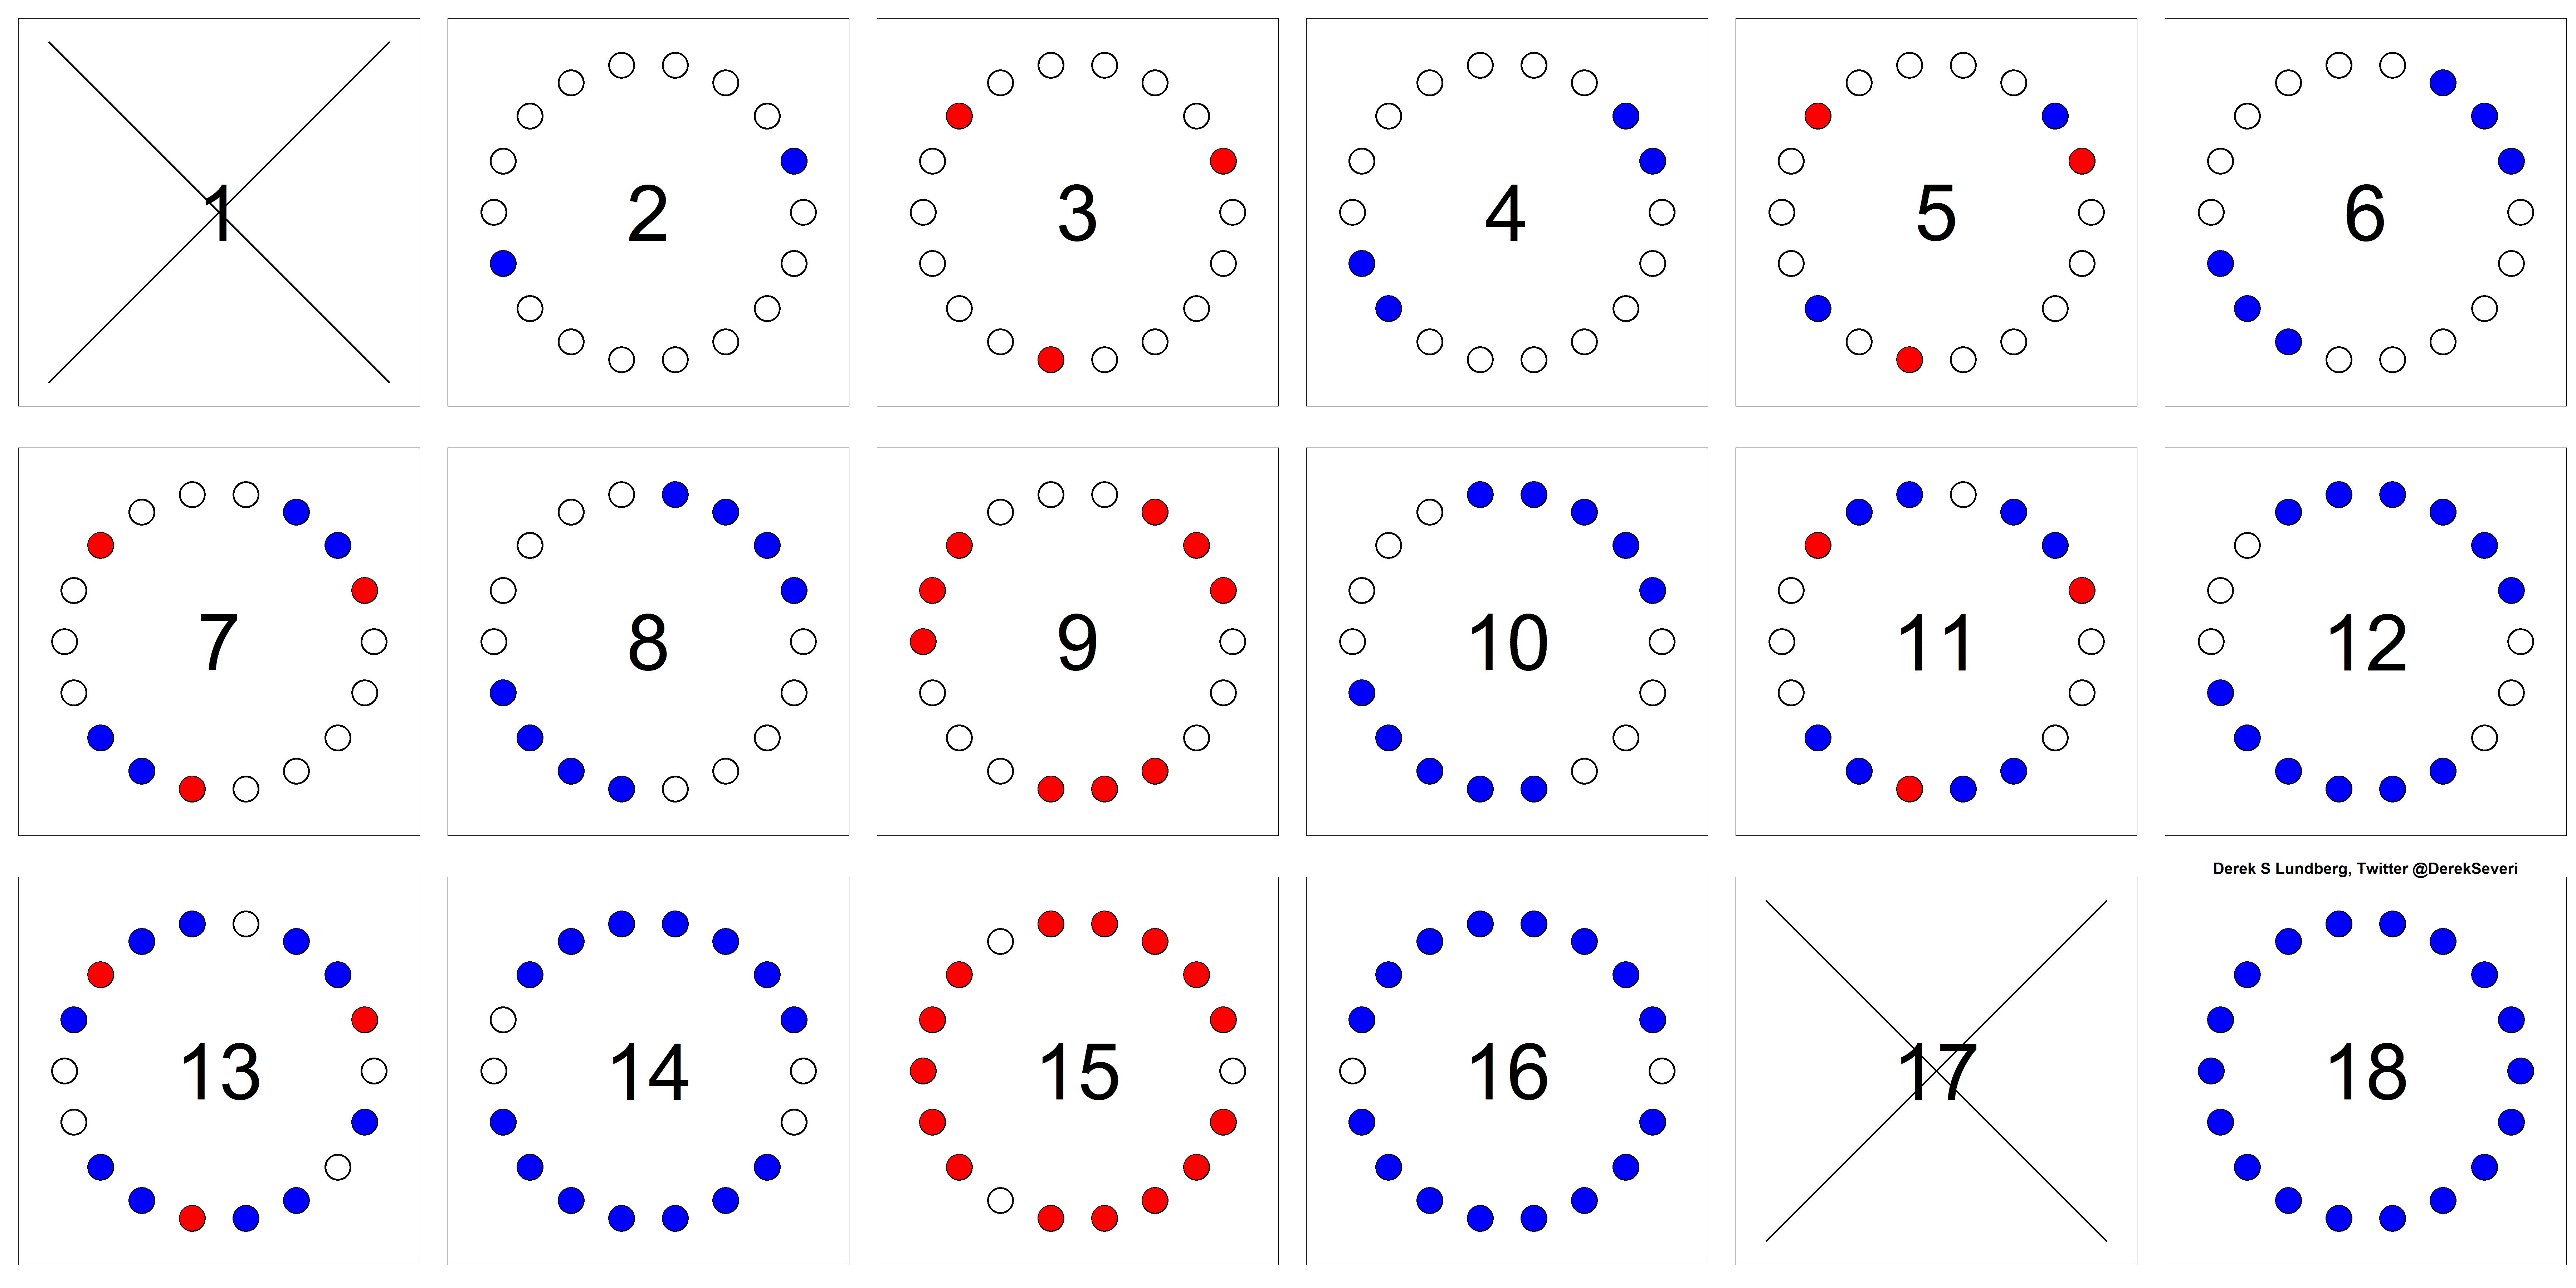
\includegraphics{figures/equipamentos/balanceamento_18.png}

}

\end{figure}

\hypertarget{balanceamento-da-centruxedfuga-de-24-amostras}{%
\subsection{Balanceamento da centrífuga de 24
amostras}\label{balanceamento-da-centruxedfuga-de-24-amostras}}

\begin{figure}[H]

{\centering 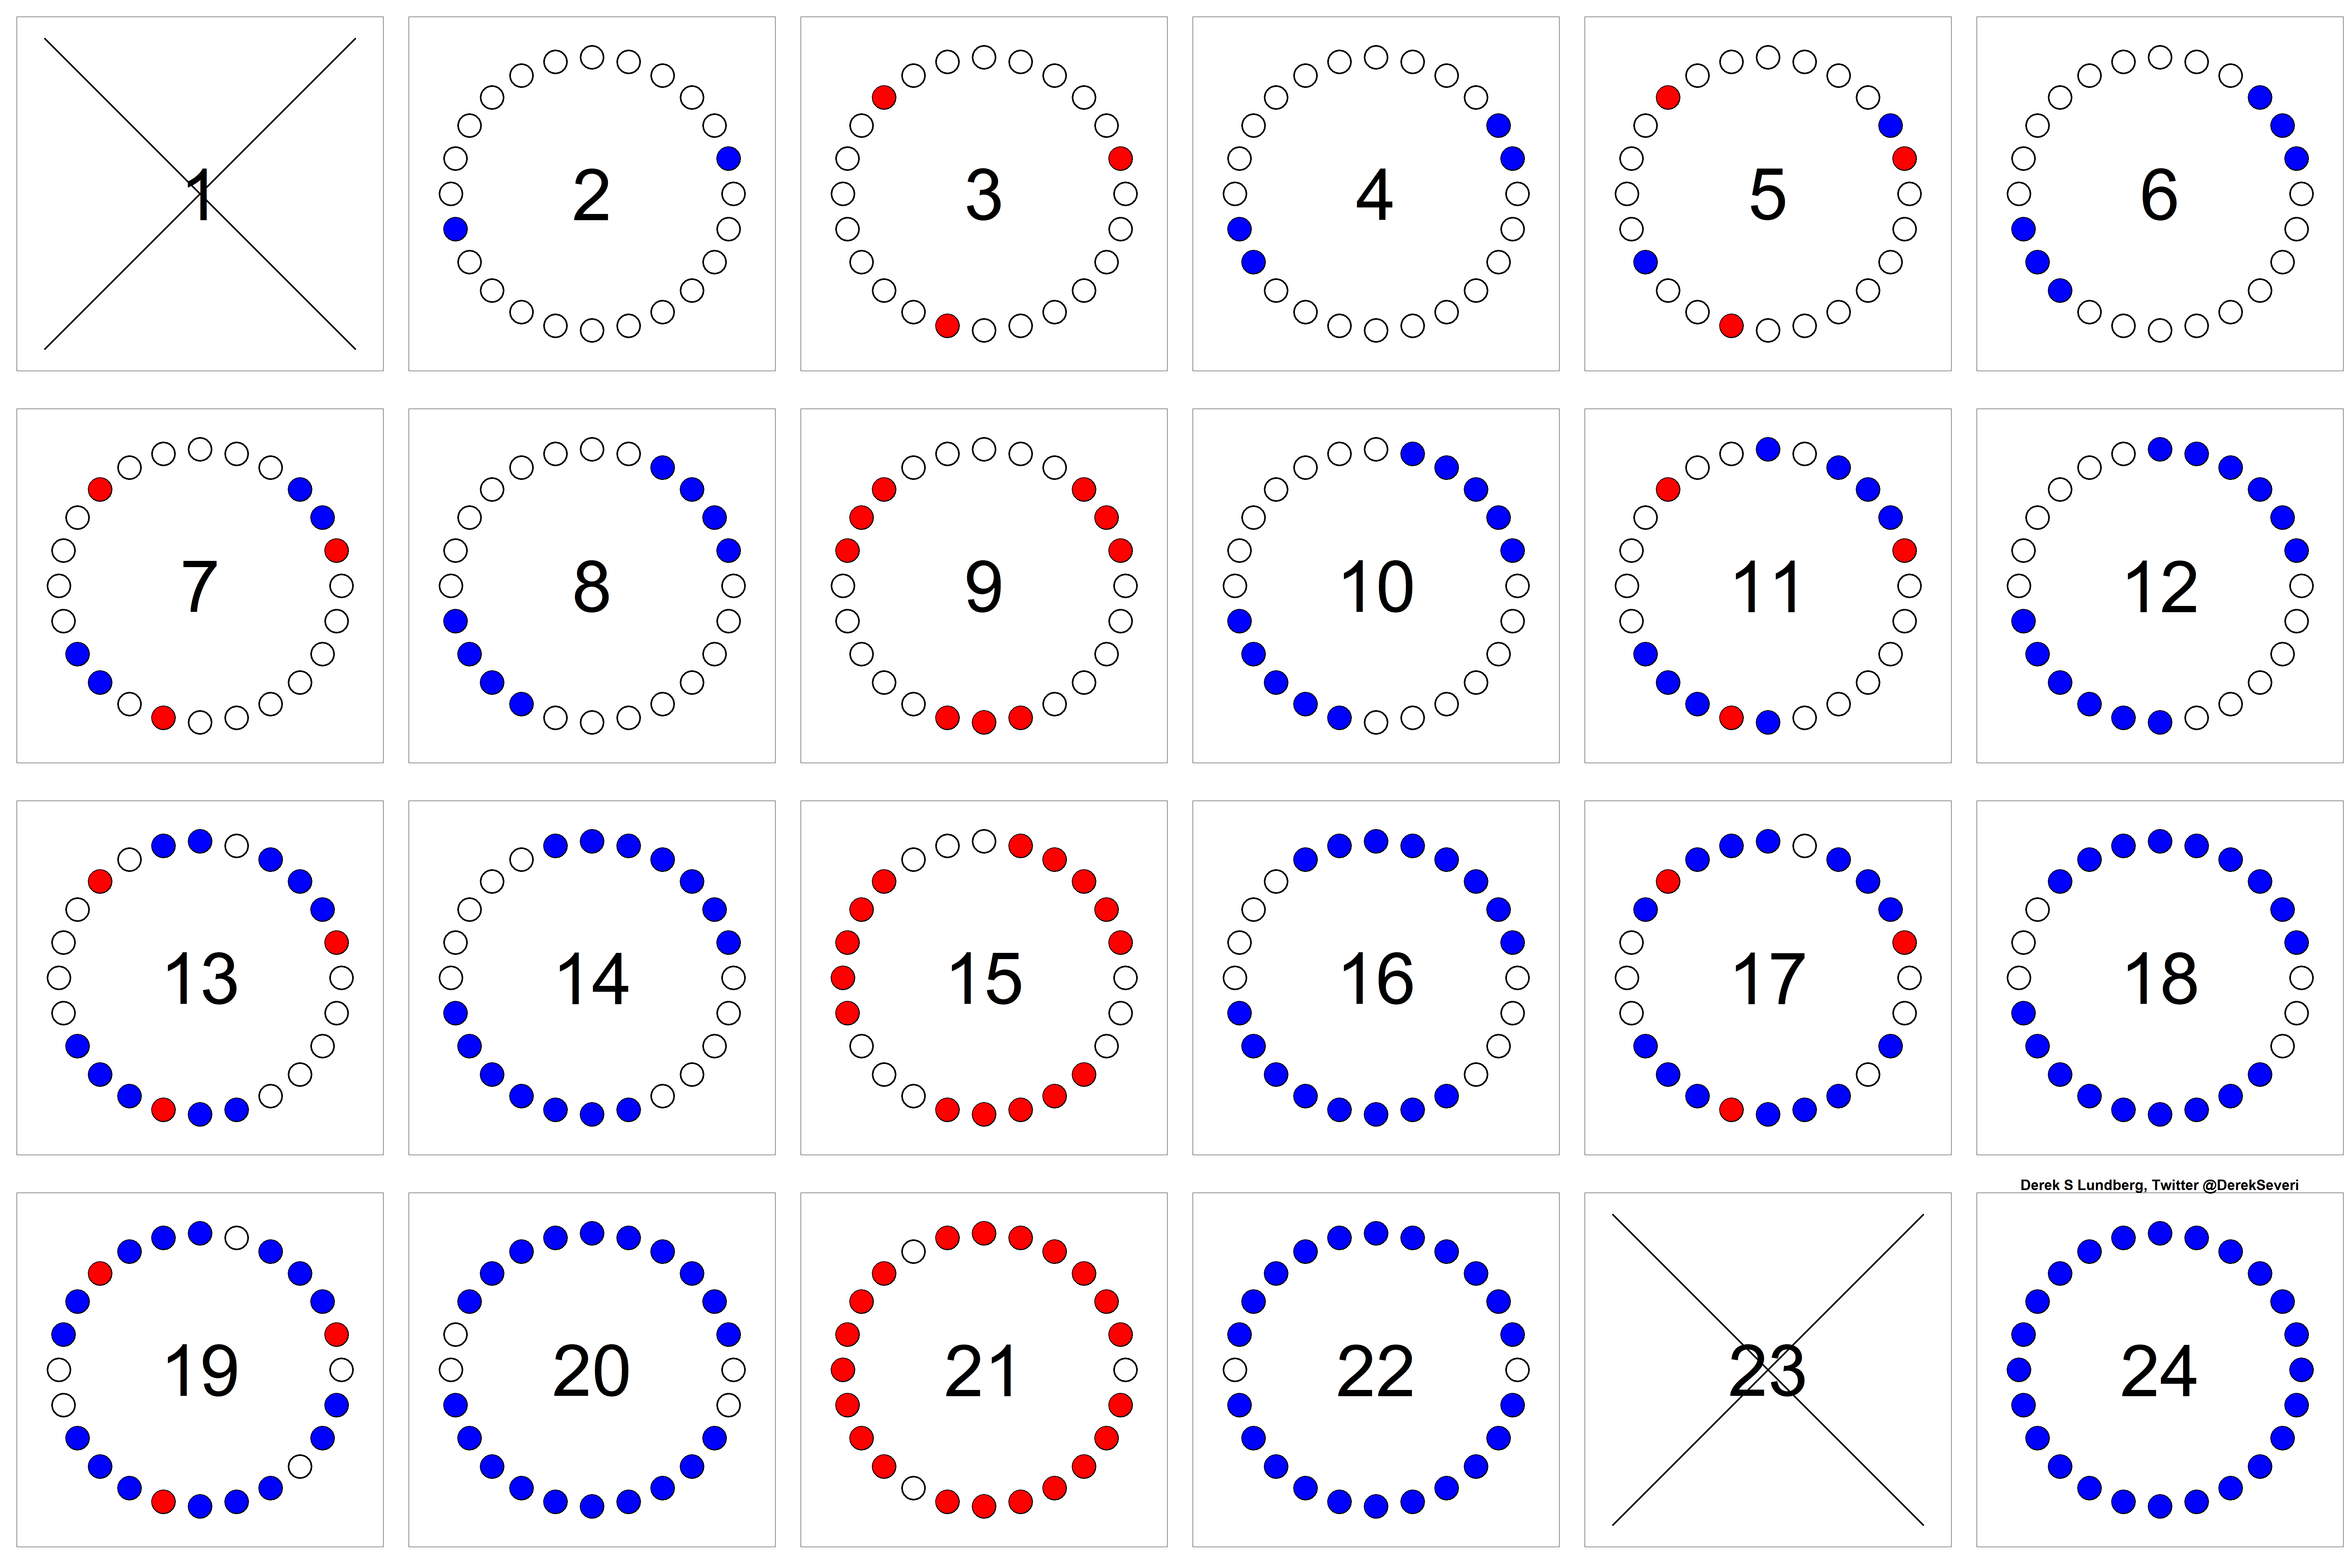
\includegraphics{figures/equipamentos/balanceamento_24.png}

}

\end{figure}

Caso ocorra uma das situações impossíveis de balanceamento, adicione um
tubo a mais sem amostra.

\end{minipage}%
\end{tcolorbox}

\hypertarget{termocicladores}{%
\section{Termocicladores}\label{termocicladores}}

O termociclador é um equipamento que automatiza o processo de
amplificação de uma sequência específica de DNA a partir de uma pequena
amostra. Possui um bloco térmico com orifícios onde tubos de 0,2 mL com
as amostras e reagentes são inseridos. O termociclador eleva e reduz a
temperatura do bloco em ciclos de tempo pré-programados, permitindo a
multiplicação em massa de moléculas de DNA com a ajuda da enzima Taq DNA
polimerase e de primers atingindo grandes quantidades de DNA após alguns
ciclos do processo. No Nupgen temos dois modelos de termocicladores:

\hypertarget{termociclador-eppendorf-mastercycler-nexus}{%
\subsection{Termociclador Eppendorf Mastercycler®
nexus}\label{termociclador-eppendorf-mastercycler-nexus}}

Nesse modelo é possível fazer apenas uma reação de PCR por vez, embora
tenha uma grande quantidade de poços (96 poços). É utilizado geralmente
quando o número de amostras a serem amplificadas ultrapassa 32, que é o
limite do outro modelo de termociclador disponível para utilização.

\begin{figure}

{\centering 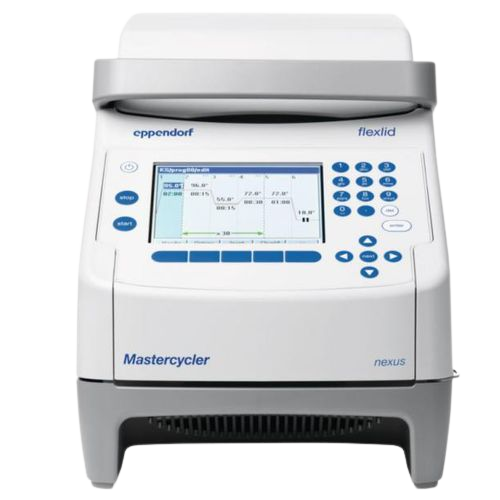
\includegraphics[width=\textwidth,height=3.125in]{figures/equipamentos/termociclador_eppendorf.png}

}

\caption{Esse termociclador encontra-se no laboratório do Bloco G90.}

\end{figure}

\hypertarget{termiciclador-applied-biosystems-proflex-3-x-32-well-pcr-system}{%
\subsection{Termiciclador Applied Biosystems® ProFlex™ 3 x 32-well PCR
System}\label{termiciclador-applied-biosystems-proflex-3-x-32-well-pcr-system}}

O sistema ProFlex™ 3 x 32-Well PCR permite executar três experimentos de
uma só vez em cada um dos blocos. Dessa maneira, é possível realizar
três PCR diferentes e independentes. No entanto, o número máximo de
amostras em cada bloco é 32. Todos os programas utilizados pelos alunos
do laboratório estão salvos nesse aparelho.

\begin{figure}

{\centering 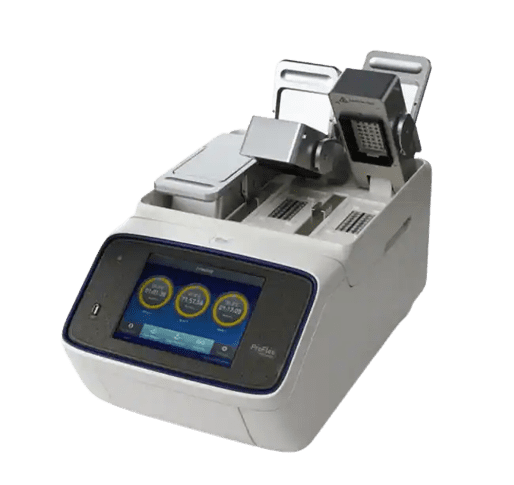
\includegraphics[width=\textwidth,height=3.125in]{figures/equipamentos/termiciclador_applied_biosystems.png}

}

\caption{Esse termociclador encontra-se no laboratório do Bloco G90.}

\end{figure}

\hypertarget{balanuxe7a-eletruxf4nica-semi-analuxedtica-320g-bl320h}{%
\section{Balança Eletrônica Semi-Analítica 320g
BL320H}\label{balanuxe7a-eletruxf4nica-semi-analuxedtica-320g-bl320h}}

A balança é um instrumento que mede a massa de um corpo. É utilizada
para pesar reagentes do laboratório que estão em pó, como a agarose.

\begin{figure}

{\centering \includegraphics[width=\textwidth,height=3.125in]{figures/equipamentos/balança.png}

}

\end{figure}

Há uma balança no laboratório do Bloco G90 e uma no laboratório do Bloco
G80.

\hypertarget{vuxf3rtex-fisherscientific-genie-2}{%
\section{Vórtex FisherScientific Genie
2}\label{vuxf3rtex-fisherscientific-genie-2}}

O agitador vórtex é utilizado para duas funções: agitar e homogeneizar
uma determinada solução líquida, contida em pequenos tubos, como os
tubos tipo eppendorf. Esse aparelho é composto por um motor que gera
movimento em um receptáculo feito em borracha sintética. Nesse
receptáculo é colocado os tubos com as substâncias que serão submetidas
à agitação. O movimento que é produzido cria um vórtice no líquido
submetido ao aparelho. Pode ser configurado para funcionar de forma
periódica ou contínua, ativado conforme a pressão do recipiente.

\begin{figure}

{\centering 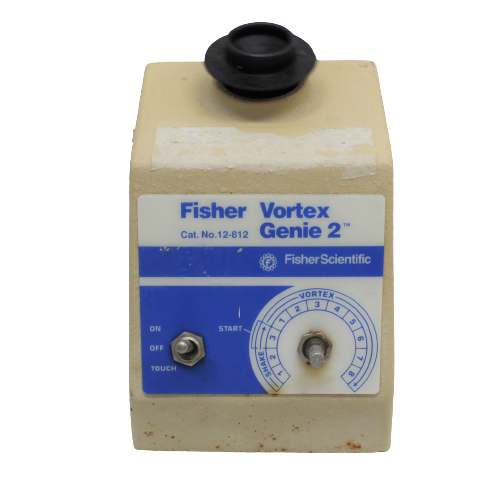
\includegraphics[width=\textwidth,height=3.125in]{figures/equipamentos/vortex.png}

}

\end{figure}

Há um vórtex no laboratório do Bloco G90 e um no laboratório do Bloco
G80.

\hypertarget{banho-maria}{%
\section{Banho maria}\label{banho-maria}}

O banho maria é um equipamento que permite a termorregulação de uma
amostra, por meio do controle da temperatura de um fluido térmico
(água), o qual é colocado dentro da cuba do banho e que irá transferir a
temperatura ajustada no banho para a amostra imersa nele. É utilizado em
etapas que necessitem do aquecimento das amostras, como durante a
extração de DNA e na purificação das amostras após a PCR. Dependendo do
procedimento a ser realizado, uma temperatura ideal deverá ser
programada no banho-maria. No Nupgen há dois modelos de banho maria
disponíveis:

\hypertarget{banho-maria-digital-solidsteel}{%
\subsection{Banho maria digital
SolidSteel}\label{banho-maria-digital-solidsteel}}

\begin{figure}

{\centering 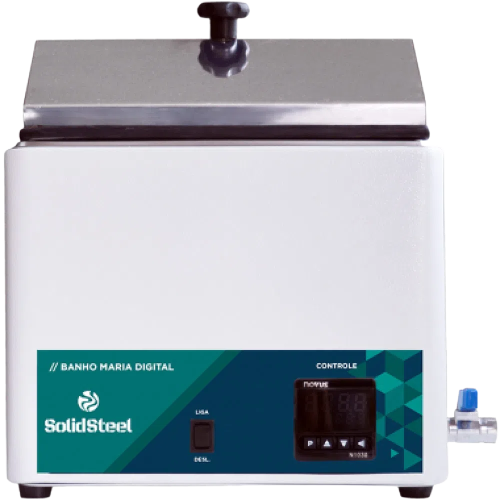
\includegraphics[width=\textwidth,height=3.125in]{figures/equipamentos/banho_maria_digital.png}

}

\caption{Esse banho maria encontra-se no laboratório do Bloco G90.}

\end{figure}

\hypertarget{banho-maria-fisherscientific-isotemp}{%
\subsection{Banho maria FisherScientific
Isotemp}\label{banho-maria-fisherscientific-isotemp}}

\begin{figure}

{\centering 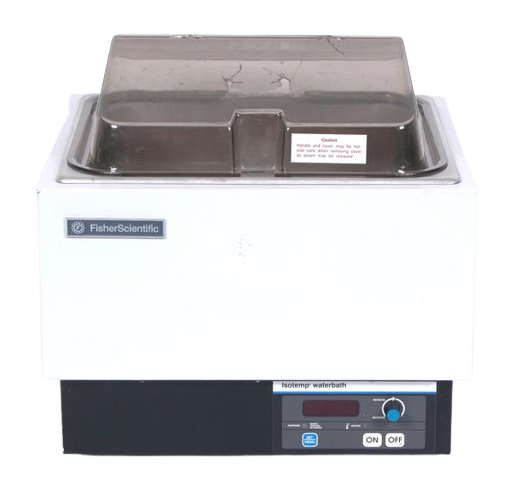
\includegraphics[width=\textwidth,height=3.125in]{figures/equipamentos/banho_maria_fischer.png}

}

\caption{Esse banho maria encontra-se no laboratório do Bloco G80.}

\end{figure}

\hypertarget{transiluminadores}{%
\section{Transiluminadores}\label{transiluminadores}}

Serve para visualizar o resultado após eletroforese em gel de agarose
utilizando um corante específico para o tipo de luz (LED ou UV). Há dois
tipos de transiluminadores no Nupgen:

\hypertarget{transiluminador-de-luz-led-kasvi}{%
\subsection{Transiluminador de luz LED
Kasvi}\label{transiluminador-de-luz-led-kasvi}}

O transiluminador LED é um equipamento leve e com design moderno, além
de ser uma inovação na área de eletroforese. Ao contrário dos
transiluminadores tradicionais com luz UV, a iluminação de LED não causa
deterioração da amostra e não é nociva ao usuário. Acompanha câmara
escura que permite documentar e arquivar rapidamente imagens dos géis
através de câmeras fotográficas comuns, inclusive câmeras de telefones
celulares. Para visualizar o gel nesse aparelho é necessário utilizar o
corante Safer, específico para esse tipo de luz.

\begin{figure}

{\centering 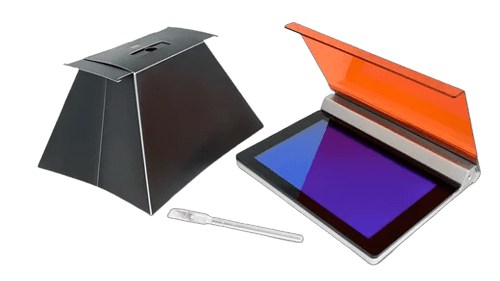
\includegraphics[width=\textwidth,height=3.125in]{figures/equipamentos/transiluminador_led.png}

}

\caption{Esse transiluminador encontra-se no laboratório do Bloco G90.}

\end{figure}

\hypertarget{transiluminador-de-luz-uv}{%
\subsection{Transiluminador de luz UV}\label{transiluminador-de-luz-uv}}

Para visualizar o gel nesse aparelho é necessário utilizar o corante
GelRed, específico para esse tipo de luz. Coloca-se uma câmara escura
sobre o aparelho para possibilitar o registro fotográfico, além de
proteger da luz UV que é emitida, visto que é nociva para a saúde
humana. Portanto, não deve-se olhar o gel com a luz ligada sem as
devidas proteções.

\begin{figure}

{\centering 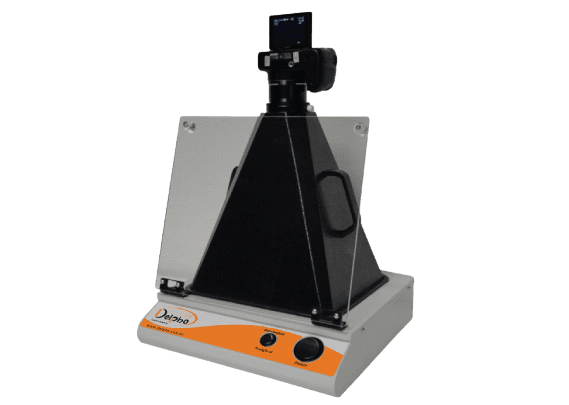
\includegraphics[width=\textwidth,height=3.125in]{figures/equipamentos/transiluminador_uv.png}

}

\caption{Esse transiluminador encontra-se no laboratório do Bloco G80.}

\end{figure}

\hypertarget{microondas}{%
\section{Microondas}\label{microondas}}

O microondas é utilizado para aquecer soluções, principalmente no
preparo do gel de agarose, visto que é necessário o aquecimento para
completa homogeneização. Quando o gel é reutilizado, também é derretido
no microondas antes de ser despejado na cuba.

\begin{figure}

{\centering 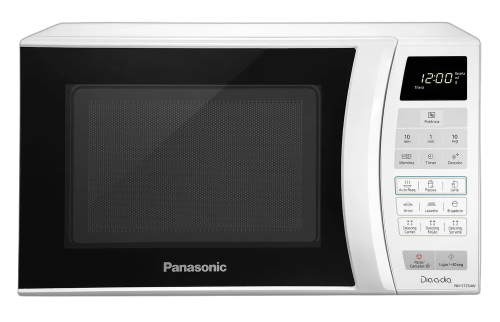
\includegraphics[width=\textwidth,height=3.125in]{figures/equipamentos/Microondas.png}

}

\end{figure}

Há um microondas no laboratório do Bloco G90 e um no laboratório do
Bloco G80.

\hypertarget{cuba-de-eletroforese-horizontal}{%
\section{Cuba de eletroforese
horizontal}\label{cuba-de-eletroforese-horizontal}}

A cuba de eletroforese é utilizada na separação de proteínas e ácidos
nucleicos, assim como nas análises de fragmentos amplificados por meio
da PCR.

\begin{figure}

{\centering 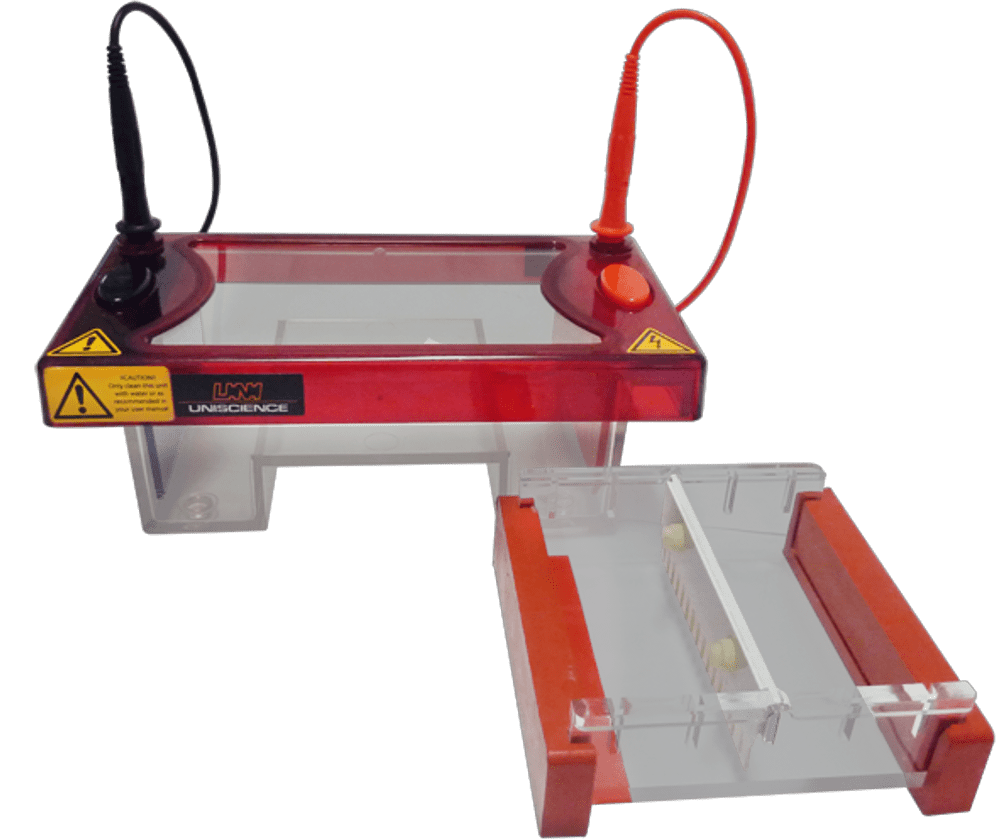
\includegraphics[width=\textwidth,height=3.125in]{figures/equipamentos/cuba_eletroforese_horizontal.png}

}

\end{figure}

Há uma cuba no laboratório do Bloco G90 e uma no laboratório do Bloco
G80.

\hypertarget{fonte-para-eletroforese}{%
\section{Fonte para eletroforese}\label{fonte-para-eletroforese}}

A fonte é utilizada para ligar os cabos de energia à cuba de
eletroforese e fornecer energia elétrica para a corrida do gel. É
adequada de acordo com a voltagem desejada para a corrida (por exemplo,
100V). Algumas permitem a programação do tempo também.

\begin{figure}

\begin{minipage}[t]{0.50\linewidth}

{\centering 

\raisebox{-\height}{

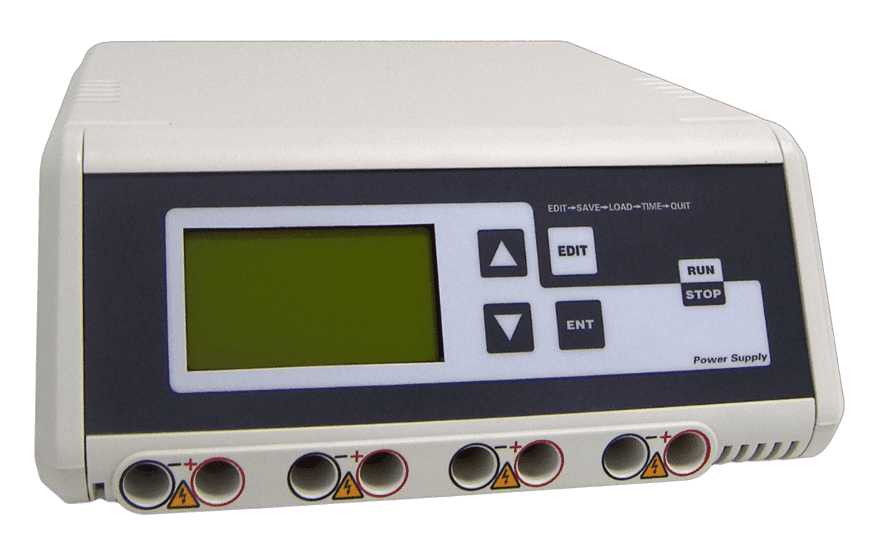
\includegraphics{figures/equipamentos/Fonte para eletroforese.png}

}

}

\end{minipage}%
%
\begin{minipage}[t]{0.50\linewidth}

{\centering 

\raisebox{-\height}{

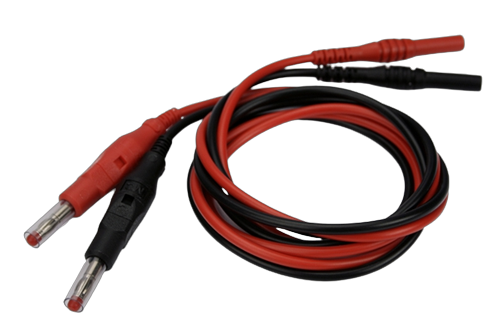
\includegraphics{figures/equipamentos/Fonte para eletroforese2.png}

}

}

\end{minipage}%

\end{figure}

Há uma fonte no laboratório do Bloco G90 e uma no laboratório do Bloco
G80.

\hypertarget{estufas}{%
\section{Estufas}\label{estufas}}

O uso mais básico de uma estufa de laboratório é para secar e
esterilizar equipamentos, geralmente vidrarias. Também é utilizada para
secar amostras que necessitam desse processo durante o protocolo (por
exemplo, envio para o sequenciamento). As estufas usam convecção térmica
para fornecer calor à câmara, o que permite manter temperaturas
uniformes.

\hypertarget{mini-estufa}{%
\subsection{Mini estufa}\label{mini-estufa}}

A mini estufa é utilizada para secagem das amostras. Seu tamanho
compacto é ideal para secar os tubos na purificação e para o envio das
amostras para o sequenciamento.

\begin{figure}

{\centering 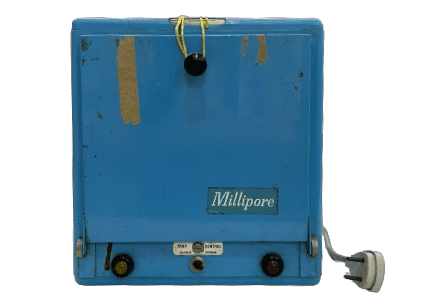
\includegraphics[width=\textwidth,height=3.125in]{figures/equipamentos/estufa_pequena.png}

}

\caption{Essa estufa encontra-se no laboratório do Bloco G90.}

\end{figure}

\hypertarget{estufa-grande}{%
\subsection{Estufa grande}\label{estufa-grande}}

Essa estufa é mais utilizada na secagem de vidrarias ou outros
utensílios do laboratório que necessitem, visto que seu tamanho é maior.
No entanto, também pode ser utilizada para secagem de amostras quando
necessário (durante a extração de DNA, por exemplo).

\begin{figure}

{\centering 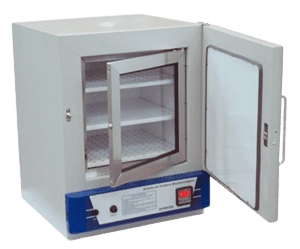
\includegraphics[width=\textwidth,height=3.125in]{figures/equipamentos/estufa_grande.png}

}

\caption{Essa estufa encontra-se no laboratório do Bloco G80.}

\end{figure}

\hypertarget{agitador-magnuxe9tico}{%
\section{Agitador magnético}\label{agitador-magnuxe9tico}}

O Agitador magnético é um equipamento de laboratório utilizado para
realizar misturas de diversas soluções. Para que a mistura aconteça, é
colocado dentro do recipiente uma pulga (barra magnética), que irá fazer
a agitação do líquido enquanto o aparelho estiver ligado. O agitador
funciona como um ímã que gira acoplado a um motor elétrico, mexendo
consequentemente a pulga promovendo a mistura da solução. É mais
utilizado no preparado de tampão TBE estoque, visto que é necessário uma
boa homogeneização da solução.

\begin{figure}

{\centering 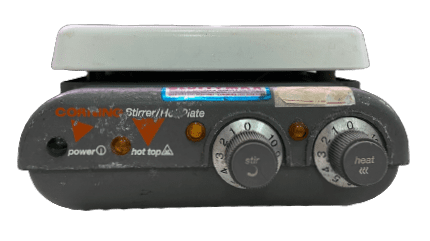
\includegraphics[width=\textwidth,height=3.125in]{figures/equipamentos/agitador_magnetico.png}

}

\end{figure}

Esse agitador/pulga encontra-se no laboratório do Bloco G90.

\bookmarksetup{startatroot}

\hypertarget{biosseguranuxe7a}{%
\chapter{Biossegurança}\label{biosseguranuxe7a}}

Falar sobre biossegurança no lab

Limpeza, contaminação, perigos, EPI, etc

Produtos perigosos: Ácido bórica

\bookmarksetup{startatroot}

\hypertarget{coletas}{%
\chapter{Coletas}\label{coletas}}

Todos os trabalhos do laboratório começam com a coleta de material
biológico, por isso é fundamental que essa etapa seja feita de forma
correta para não prejudicar os processos seguintes. Muito cuidado deve
ser tomado desde o planejamento da coleta até sobre as informações
registradas.

No Nupgen realizamos diversas coletas de peixes, caramujos, macrófitas e
até de água. O PELD é um projeto que facilita bastante este processo de
coleta.

\hypertarget{campo}{%
\section{Campo}\label{campo}}

Toda viagem de campo é bem complicada, pois temos que fazer várias
coisas com antecedência e não podemos esquecer nada.

\hypertarget{licenuxe7a-de-coleta}{%
\subsection{Licença de coleta}\label{licenuxe7a-de-coleta}}

Toda coleta de material biológico deve ter uma licença de coleta, pois
retirar animais silvestres da natureza é crime. Por isso é essencial
conversar com os professores responsáveis antes e providenciar. Leve a
autorização impressa dentro de um saco plástico transparente para não
molhar. O PELD já possui uma licença geral de coleta.

\hypertarget{local-de-coleta}{%
\subsection{Local de coleta}\label{local-de-coleta}}

Definir o local que será realizada a coleta é muito importante, pois
quanto melhor o local, menos esforço amostral será necessário e,
consequentemente, menos dinheiro será gasto. Converse com outras pessoas
que já realizaram coletas no mesmo ambiente previamente.

É muito importante conhecer o ponto de coleta, bem como planejar a
infraestrutura, alimentação e quantas pessoas serão necessárias.

Preparação para viagem

\hypertarget{dados}{%
\section{Dados}\label{dados}}

Em qualquer coleta deve ser registrado o maior número de dados possível,
afim de facilitar o trabalho futuro ou mesmo para prever possíveis
questionamentos de revisores. Alguns dados muito importante são:

\begin{itemize}
\item
  Coordenadas;
\item
  Espécie coletada;
\item
  Número de espécimes;
\item
  Local;
\item
  Fotos e descrição do ambiente;
\end{itemize}

\hypertarget{triagem}{%
\section{Triagem}\label{triagem}}

Após coletar os espécimes, é necessário realizar a triagem para garantir
a qualidade do estudo. Com caramujos geralmente são triados os
parasitos, com peixes podemos retirar o tecido, etc.

\part{Protocolos}

\hypertarget{diluiuxe7uxf5es}{%
\chapter{Diluições}\label{diluiuxe7uxf5es}}

As diluições são um procedimento comum em laboratório que consiste em
misturar uma solução concentrada com uma solução diluente para produzir
uma solução de concentração conhecida. Elas são utilizadas em diversas
aplicações em laboratório, como preparação de amostras para análises
químicas ou biológicas, padronização de soluções e muito mais.

Para realizar uma diluição, é necessário conhecer a concentração da
solução inicial e a quantidade de solução diluente que será adicionada.
A concentração da solução final pode ser calculada usando a fórmula de
diluição:

\(C1 * V1 = C2 * V2\)

Onde \(C1\) é a concentração da solução inicial, \(V1\) é o volume da
solução inicial, \(C2\) é a concentração da solução final e \(V2\) é o
volume da solução final.

\hypertarget{etanol}{%
\section{Etanol}\label{etanol}}

\hypertarget{etanol-70}\label{etanol-70}}

\textbf{Para preparar 100ml}

Em um tubo tipo falcon, adicionar:

\begin{itemize}
\item
  70 mL de etanol absoluto
\item
  30 mL de água destilada
\end{itemize}

\hypertarget{etanol-80}\label{etanol-80}}

\textbf{Para preparar 100ml}

Em um tubo tipo falcon, adicionar:

\begin{itemize}
\item
  80 mL de etanol absoluto
\item
  20 mL de água destilada
\end{itemize}

\hypertarget{gelred}{%
\section{GelRed}\label{gelred}}

\textbf{Para preparar 500 μL}

Em um tubo de 1,5 mL envolto com fita e papel alumínio, adicionar:

\begin{itemize}
\item
  1 μL de GelRed (estoque)
\item
  499 μL de água ultrapura (Milli-Q)
\end{itemize}

\hypertarget{ladder-100pb}{%
\section{Ladder 100pb}\label{ladder-100pb}}

\textbf{Para preparar 100 μL}

Em um tubo de 1,5 mL, adicionar:

\begin{itemize}
\item
  10 μL de Ladder (estoque 0,5 μg/μL)
\item
  90 μL de água ultrapura (Milli-Q)
\end{itemize}

\hypertarget{lambda}{%
\section{Lambda}\label{lambda}}

\hypertarget{lambda-5ngux3bcl-para-1000-ux3bcl}{%
\subsection{Lambda 5ng/μL (para 1000
μL)}\label{lambda-5ngux3bcl-para-1000-ux3bcl}}

\begin{itemize}
\item
  9,27 μL de lambda (conferir concentração)
\item
  990,73 μL de água ultrapura (Milli-Q)
\end{itemize}

\hypertarget{lambda-10ngux3bcl-para-1000-ux3bcl}{%
\subsection{Lambda 10ng/μL (para 1000
μL)}\label{lambda-10ngux3bcl-para-1000-ux3bcl}}

\begin{itemize}
\item
  18,56 μL de lambda
\item
  981,44 μL de água ultrapura (Milli-Q)
\end{itemize}

\hypertarget{lambda-20ngux3bcl-para-1000-ux3bcl}{%
\subsection{Lambda 20ng/μL (para 1000
μL)}\label{lambda-20ngux3bcl-para-1000-ux3bcl}}

\begin{itemize}
\item
  37,11 μL de lambda
\item
  962,89 μL de água ultrapura (Milli-Q)
\end{itemize}

\hypertarget{primer-para-uso-10-ux3bcm}{%
\section{Primer para uso (10 μM)}\label{primer-para-uso-10-ux3bcm}}

\textbf{Para preparar 60 μL}

Em um tubo, adicionar:

\begin{itemize}
\item
  10 μL do primer estoque (60 μM - conferir concentração)
\item
  50 μL de água ultrapura (Milli-Q)
\end{itemize}

\hypertarget{proteinase-k-20-mgml}{%
\section{Proteinase K 20 mg/mL}\label{proteinase-k-20-mgml}}

\textbf{Para preparar 1 mL}

\begin{itemize}
\item
  20 mg de Proteinase K (estoque)
\item
  1 mL de água ultrapura (Milli-Q)
\end{itemize}

\textbf{Modo de preparo:} lavar bem uma espátula, fazer a desinfecção
com álcool 70\% e pesar a Proteinase K em um microtubo novo (1,5 mL).
Adicionar a água ultrapura (Milli-Q) e ressuspender bem com a pipeta.
Agitar a solução no vórtex para homogeneizar bem. Manter no freezer.

\hypertarget{tampuxe3o-tbe-5x-estoque}{%
\section{Tampão TBE 5x (estoque)}\label{tampuxe3o-tbe-5x-estoque}}

\textbf{Para preparar 1000 mL}

\begin{itemize}
\item
  54 g de Tris-Base
\item
  27,5 g de Ácido Bórico
\item
  20 mL de EDTA 0,5M pH 8,0
\end{itemize}

Completar para 1000 mL com água destilada

\textbf{Modo de preparo:} em um becker, adicionar um pouco da água
destilada. Ir adicionando aos poucos os reagentes, utilizando o agitador
magnético para homogeneizar a solução. Ao final, utilizando uma proveta,
completar o volume de água que falta e armazenar em frascos de vidro
(tampa laranja). Etiquetar e autoclavar.

\hypertarget{tampuxe3o-tbe-1x-corrida-eletroforuxe9tica}{%
\section{Tampão TBE 1x (corrida
eletroforética)}\label{tampuxe3o-tbe-1x-corrida-eletroforuxe9tica}}

\textbf{Para preparar 1000 mL}

\(C1 * V1 = C2 * V2\)

5(estoque) * V1 = 1 * 1000 mL

V1 = 1000/5

V1 = 200 mL de TBE 5x

Completar para 1000 mL de água destilada (= 800 mL)

\hypertarget{tampuxe3o-coleta-macruxf3fitas}{%
\section{Tampão Coleta
Macrófitas}\label{tampuxe3o-coleta-macruxf3fitas}}

\textbf{Para preparar 1000 mL}

\begin{itemize}
\item
  Tris HCl - 10 mL
\item
  EDTA (0,5mM) - 2 mL
\item
  Água destilada - 988ml
\end{itemize}

pH = 8,0

\textbf{Modo de preparo:} Colocar 10ml do Tris HCl e 2ml do EDTA (0,5mM)
em um frasco de vidro (tampa laranja ou azul), completar o volume com
água destilada. Agitar o frasco para misturar bem e medir o pH com as
fitinhas, para conferir se está correto; caso não esteja, basta ajustar
com as soluções para pH. Etiquetar e autoclavar.

\hypertarget{peg-20-nacl-25m}{%
\section{PEG 20\% NaCl 2,5M}\label{peg-20-nacl-25m}}

\textbf{Para preparar 75 mL}

\begin{itemize}
\item
  15 g de Polietilenoglicol
\item
  10,95 g de NaCl
\end{itemize}

Completar o volume para 75 mL com água ultrapura (Milli-Q)

\textbf{Modo de preparo:} colocar em um becker um pouco da água
ultrapura e misturar o Polietilenoglicol e o NaCl com um bastão de vidro
até a solução ficar homogênea. Depois de homogeneizada, completar o
volume de água para 75 mL e com o auxílio de uma seringa passar a
solução por um filtro (0,2 µM -- azul). Acondicionar em tubos Falcon
para autoclavar. Após autoclavado, fazer alíquotas em microtubos de 1,5
mL. Manter no freezer da geladeira.

\hypertarget{diluiuxe7uxe3o-de-primer-liofilizado}{%
\section{Diluição de primer
liofilizado}\label{diluiuxe7uxe3o-de-primer-liofilizado}}

\textbf{Quantidade em nmol x 1000 / 60 = Quantidade de água ultrapura
(Milli-Q)}

Acrescentar a quantidade obtida de água diretamente no tubo do primer
liofilizado.

Obs: 60 µM é a concentração utilizada para diluição dos primers no
laboratório.

\hypertarget{extrauxe7uxe3o}{%
\chapter{Extração}\label{extrauxe7uxe3o}}

A extração de DNA é um processo fundamental em genética molecular que
consiste em separar o material genético de uma célula ou tecido para que
possa ser estudado e manipulado. Existem várias técnicas de extração de
DNA, mas todas elas envolvem a lise da célula para liberar o DNA e a
purificação do DNA para remover contaminantes. Para que seja possível
conseguir DNA de boa qualidade, existem protocolos que foram testados,
adaptados e otimizados para cada grupo estudado no laboratório.

A primeira etapa da extração de DNA é a lise da célula, que pode ser
feita de várias maneiras, como maceração mecânica, lise com detergentes
ou lise com enzimas (como a Proteinase K). Na maioria dos protocolos
utilizados para extração de DNA no Nupgen os três métodos de lise
celular são combinados, ou seja, é primeiramente realizada a maceração
mecânica, adicionado tampão que contém detergentes que atuam nos
lipídios das membranas promovendo o seu rompimento e posteriormente a
enzima Proteinase K também é adicionada.

Após a lise das células, o DNA precisa ser separado dos restos celulares
e das proteínas. Dessa maneira, o DNA é purificado por meio de
precipitação com etanol ou cloreto de sódio, ou por meio de
centrifugação em colunas. Uma vez que o DNA é purificado, ele pode ser
utilizado em várias aplicações, como sequenciamento de DNA, clonagem,
análise de expressão gênica e muito mais. No entanto, é importante
lembrar que o DNA é um material frágil e pode ser danificado facilmente,
portanto, é importante tomar cuidado durante todo o processo de extração
e manipulação.

\begin{tcolorbox}[enhanced jigsaw, colback=white, toprule=.15mm, rightrule=.15mm, opacityback=0, left=2mm, arc=.35mm, bottomrule=.15mm, breakable, leftrule=.75mm]
\begin{minipage}[t]{5.5mm}
\textcolor{quarto-callout-note-color}{\faInfo}
\end{minipage}%
\begin{minipage}[t]{\textwidth - 5.5mm}

\textbf{Como fazemos}\vspace{2mm}

Atualmente no Nupgen são utilizados dois kits de extração diferentes:
\textbf{Wizard® Genomic DNA Purification Kit (Promega®)} e
\textbf{DNeasy® Blood and Tissue Kit (QIAGEN®)}. A escolha do kit irá
depender do organismo a ser estudado, por exemplo, para peixes,
gastrópodes e macrófitas recomenda-se a utilização do kit da Promega e
para organismos menores, como parasitas, o kit em colunas da QIAGEN é o
mais ideal.

\end{minipage}%
\end{tcolorbox}

\begin{figure}

\begin{minipage}[t]{0.50\linewidth}

{\centering 

\raisebox{-\height}{

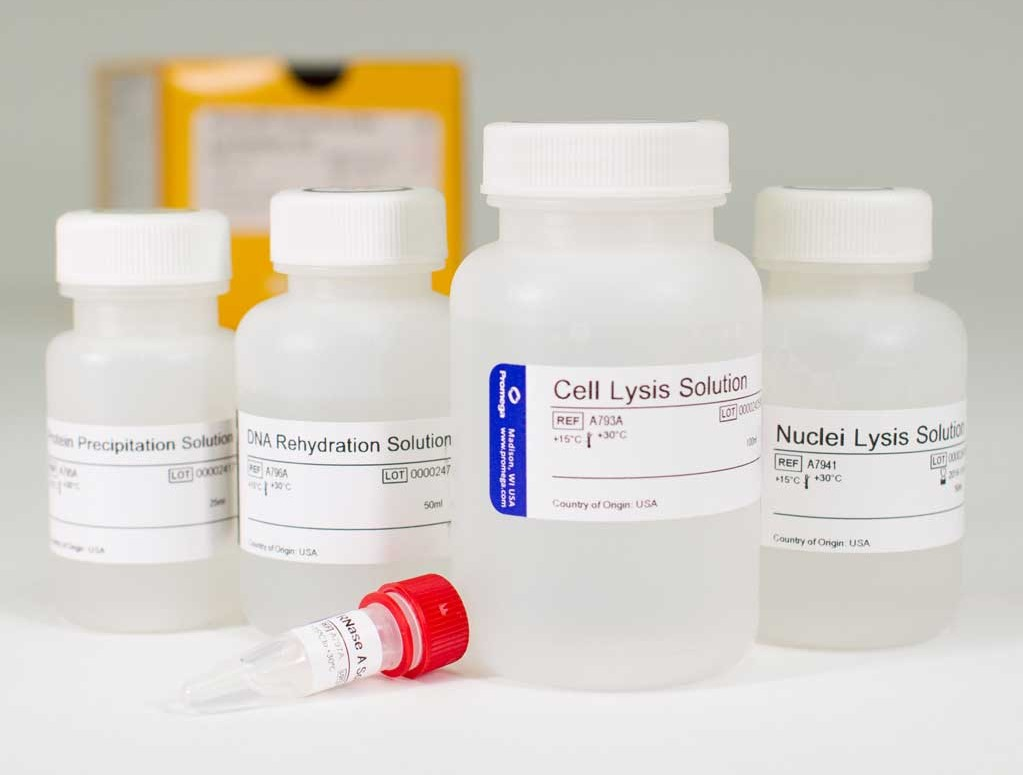
\includegraphics{figures/promega-kit.jpg}

}

\caption{Wizard® Genomic DNA Purification Kit (Promega®)}

}

\end{minipage}%
%
\begin{minipage}[t]{0.50\linewidth}

{\centering 

\raisebox{-\height}{

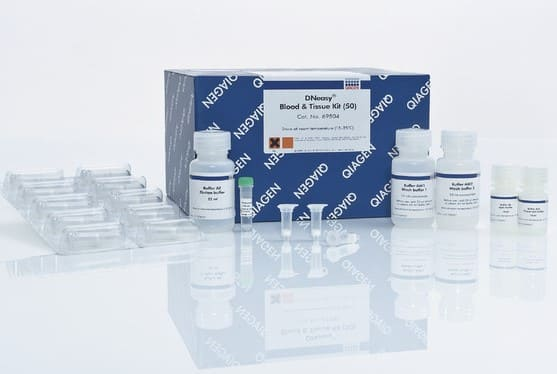
\includegraphics{figures/qiagen-kit.jpeg}

}

\caption{DNeasy® Blood and Tissue Kit (QIAGEN®)}

}

\end{minipage}%

\end{figure}

\hypertarget{protocolo-de-extrauxe7uxe3o-de-dna---promega-peixes}{%
\section{\texorpdfstring{Protocolo de Extração de DNA - Promega
\textbf{Peixes}}{Protocolo de Extração de DNA - Promega Peixes}}\label{protocolo-de-extrauxe7uxe3o-de-dna---promega-peixes}}

\begin{enumerate}
\def\labelenumi{\arabic{enumi}.}
\item
  Com pinça e bisturi, fracionar aproximadamente 20 mg de músculo.
\item
  Adicionar 400 μL de Nuclei Lysis Solution.
\item
  Incubar por 30 minutos a 55º C.
\item
  Adicionar 10 μL de Proteinase K 20 mg/ml.
\item
  Incubar a 55º C overnight ou de 2-3 horas até ficar homogêneo.
\item
  Adicionar 2 μL de RNAse Kit Solution e mexer a amostra por inversão.
\item
  Incubar 30 minutos a 37º C.
\item
  Deixar em temperatura ambiente por 5 minutos.
\item
  Adicionar 200 μL de Protein Precipitation Solution e agitar por 20
  segundos.
\item
  Deixar no gelo por 5 minutos.
\item
  Centrifugar por 10 minutos a 12.000 rpm.
\item
  Remover o sobrenadante transferindo para um tubo novo -- descartar o
  pellet.
\item
  Adicionar 600 μL de isopropanol e agitar por inversão.
\item
  Centrifugar por 2 minutos a 12.000 rpm -- descartar o sobrenadante.
\item
  Adicionar 600 μL de etanol 70\% a temperatura ambiente.
\item
  Centrifugar por 2 minutos a 12.000 rpm -- descartar sobrenadante.
\item
  Deixar secar -- pode ser na estufa.
\item
  Ressuspender em 30 μL de DNA Rehidration Solution. Deixar por 1 hora
  no banho a 65º C ou overnight a 4º C.
\end{enumerate}

\hypertarget{protocolo-de-extrauxe7uxe3o-de-dna---promega-caramujos}{%
\section{\texorpdfstring{Protocolo de Extração de DNA - Promega
\textbf{Caramujos}}{Protocolo de Extração de DNA - Promega Caramujos}}\label{protocolo-de-extrauxe7uxe3o-de-dna---promega-caramujos}}

\begin{enumerate}
\def\labelenumi{\arabic{enumi}.}
\item
  Fracionar o tecido (0,5-1 cm) e adicionar em um tubo de 1,5 ml.
\item
  Adicionar 500 μl de Nuclei Lysis Solution.
\item
  Macerar o tecido com um pistilo.
\item
  Adicionar 17,5 μl de Proteinase K 20 mg/ml.
\item
  Homogeneizar com vórtex por 10 segundos.
\item
  Incubar a 55º C overnight OU incubar a 55º C por 3 horas,
  homogeneizando com vórtex a cada hora.
\item
  Adicionar 3 μl de RNase Solution à solução e misturar por inversão do
  tubo 2-5 vezes.
\item
  Incubar a 37º C por 30 minutos. Deixar as amostras esfriarem a
  temperatura ambiente por 5 minutos antes da próxima etapa.
\item
  Adicionar 200 μl de Protein Precipitation Solution e homogeneizar com
  o vórtex vigorosamente por 20 segundos.
\item
  Colocar as amostras no gelo por 5 minutos.
\item
  Centrifugar a 12.000 rpm por 4 minutos. Nesta etapa pode ser formado
  um pellet no fundo do tubo.
\item
  Remover cuidadosamente o sobrenadante contendo o DNA (não retirar o
  pellet) e transferir para um novo tubo de 1,5 ml que já contenha 600
  μl de isopropanol (temperatura ambiente).
\item
  Misturar cuidadosamente a solução por inversão até os ``fios'' de DNA
  formarem uma massa visível.
\item
  Centrifugar a 12.000 rpm por 1 minuto. O DNA ficará no fundo do tubo e
  pode ficar visível como um pequeno pellet branco. Descartar
  cuidadosamente o sobrenadante.
\item
  Adicionar 600 μl de etanol 70\% (temperatura ambiente) e misturar
  cuidadosamente a solução por inversão.
\item
  Centrifugar a 12.000 rpm por 1 minuto.
\item
  Retirar o etanol cuidadosamente com uma pipeta sem retirar o pellet.
\item
  Inverter os tubos em papel e deixar secar por 10-15 minutos.
\item
  Adicionar 30 μL de DNA Rehydration Solution e reidratar o DNA
  incubando a 65º C por 1 hora. Periodicamente misturar a solução com
  cuidado OU incubar a 4º C overnight.
\item
  Armazenar o DNA extraído a 2-8º C.
\end{enumerate}

\hypertarget{protocolo-de-extrauxe7uxe3o-de-dna---promega-macruxf3fitas}{%
\section{\texorpdfstring{Protocolo de Extração de DNA - Promega
\textbf{Macrófitas}}{Protocolo de Extração de DNA - Promega Macrófitas}}\label{protocolo-de-extrauxe7uxe3o-de-dna---promega-macruxf3fitas}}

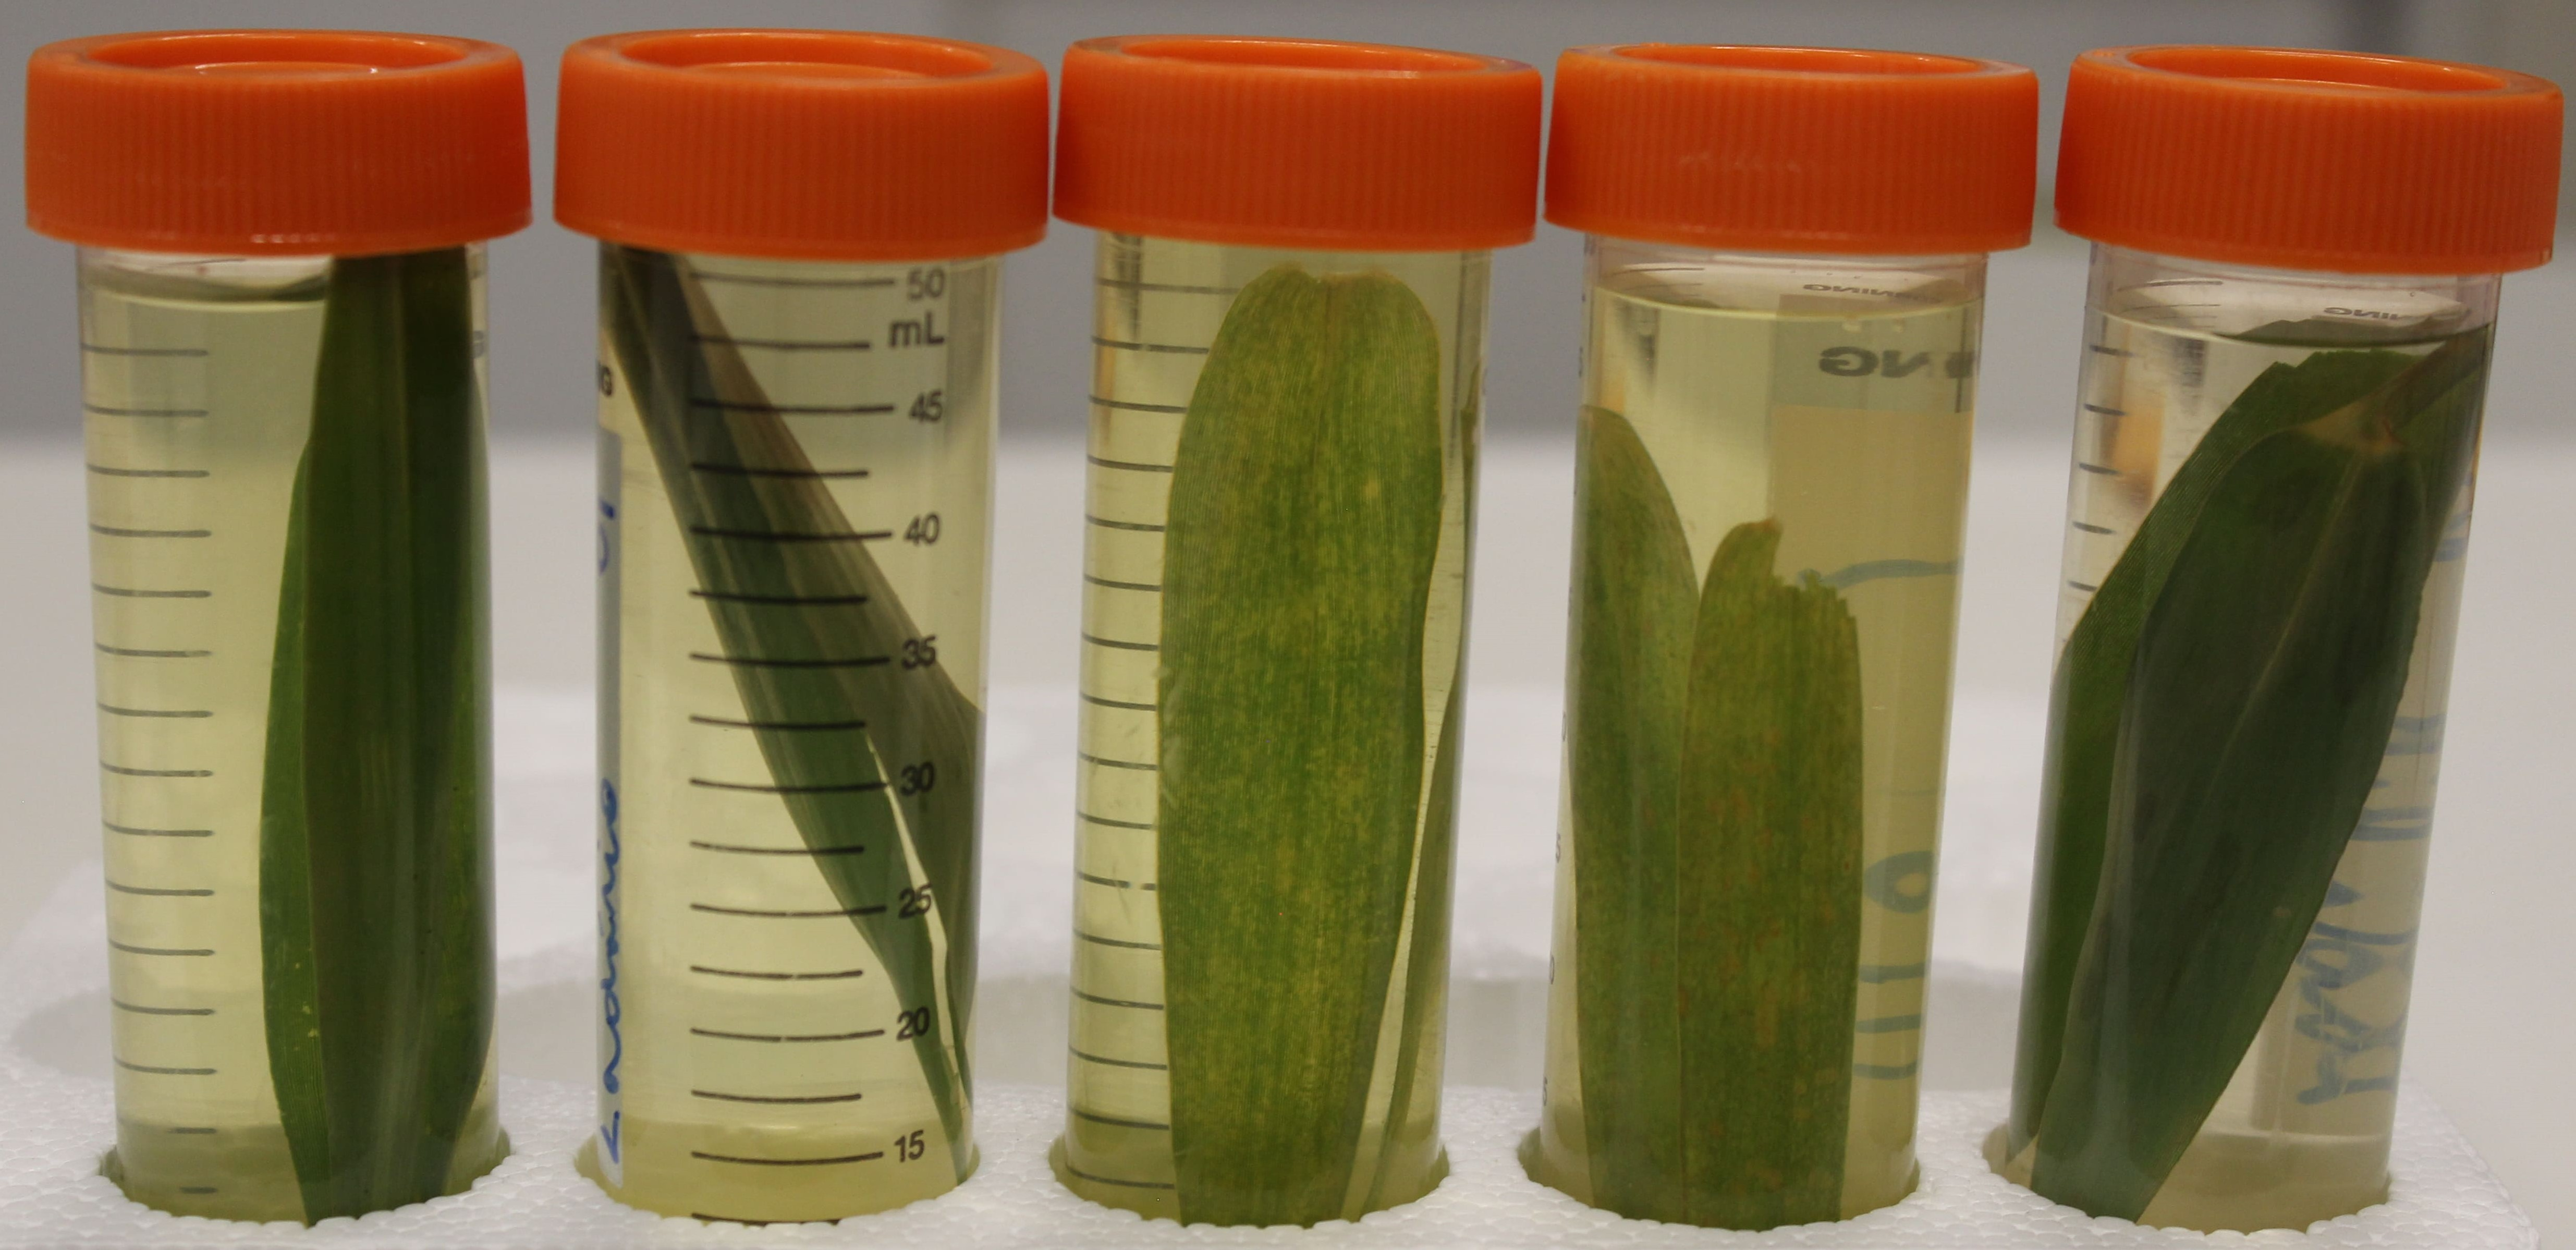
\includegraphics{figures/extracao-macrofitas.JPG}

\begin{enumerate}
\def\labelenumi{\arabic{enumi}.}
\item
  Tubos de 1,5 mL.
\item
  Amostras + nitrogênio líquido (macerar).
\item
  Adicionar 600 μl de Nuclei Lysis Solution (logo após macerar).
\item
  Banho de 15 minutos a 65° C.
\item
  Adicionar 3 μl de RNAse.
\item
  Virar o tubo 5x.
\item
  Colocar no banho por 15 minutos a 37° C (pode segurar na mão).
\item
  Deixar por 5 minutos em temperatura ambiente.
\item
  Adicionar 200 μl de Protein Precipitation Solution.
\item
  Vórtex.
\item
  Centrifugar por 3 minutos a 16.000 ou 13.000 rpm.
\item
  Separar sobrenadante e descartar o resto.
\item
  Adicionar 600 μl de isopropanol ao sobrenadante.
\item
  Virar 5x.
\item
  Centrifugar por 1 minuto a 16.000 ou 13.000 rpm.
\item
  Descartar sobrenadante.
\item
  Adicionar 600 μl de etanol 70\%.
\item
  Virar 5x.
\item
  Centrifugar por 1 minuto a 16.000 ou 13.000 rpm.
\item
  Descartar sobrenadante.
\item
  Deixar o tubo secar por 15 minutos na estufa.
\item
  Adicionar 50 μl de DNA Rehydration Solution.
\end{enumerate}

\hypertarget{protocolo-de-extrauxe7uxe3o-de-dna-com-colunas---qiagen-parasitos-e-macruxf3fitas}{%
\section{\texorpdfstring{Protocolo de Extração de DNA com Colunas -
QIAGEN \textbf{Parasitos e
Macrófitas}}{Protocolo de Extração de DNA com Colunas - QIAGEN Parasitos e Macrófitas}}\label{protocolo-de-extrauxe7uxe3o-de-dna-com-colunas---qiagen-parasitos-e-macruxf3fitas}}

\begin{enumerate}
\def\labelenumi{\arabic{enumi}.}
\item
  Deixar o mínimo possível de líquido na amostra antes de começar.
\item
  Adicionar 180 μL de Buffer ATL.
\item
  Adicionar 20 μL de proteinase K. Homogeneizar com vórtex e incubar a
  56º C até completa lise celular (30min - 2h). Homogeneizar com vórtex
  ocasionalmente durante a incubação.
\item
  Homogeneizar com vórtex por 15 segundos.
\item
  Adicionar 200 μL de Buffer AL. Homogeneizar bem com vórtex.
\item
  Adicionar 200 μL de etanol (96-100\%). Homogeneizar~ bem com vórtex.
\item
  Pipetar a mistura em uma coluna de centrifugação DNeasy Mini colocada
  em um tubo de coleta. Centrifugar a 8.000 rpm (≥6.000 x g) por 1
  minuto. Descartar o líquido filtrado e o tubo de coleta.
\item
  Colocar a coluna em um novo tubo de coleta do kit. Adicionar 500 μL de
  Buffer AW1. Centrifugar por 1 minuto a 8.000 rpm. Descartar o líquido
  filtrado e o tubo de coleta.
\item
  Colocar a coluna em um novo tubo de coleta do kit. Adicionar 500 μL de
  Buffer AW2. Centrifugar por 3 minutos a 14.000 rpm (≥20.000 x g).
  Descartar o líquido filtrado e o tubo de coleta.
\item
  Transferir a coluna para um eppendorf de 1,5 mL.
\item
  Adicionar 50 μL de Buffer AE no centro da membrana da coluna para a
  eluição do DNA. Incubar por 1 minuto a temperatura ambiente (15-25º
  C). Centrifugar por 1 minuto a 8.000 rpm.
\item
  Descartar a coluna e guardar o DNA extraído.
\end{enumerate}

\hypertarget{eletroforese}{%
\chapter{Eletroforese}\label{eletroforese}}

A eletroforese consiste em um método de separação de macromoléculas,
como o DNA, por meio da aplicação de corrente elétrica. Como as
moléculas de DNA apresentam carga negativa, quando são submetidas a um
campo elétrico, elas migram para o polo positivo, sendo este o princípio
da eletroforese, ou seja, moléculas com cargas distintas irão migrar
pelo gel de um polo a outro. Além disso, quanto menor for o tamanho da
molécula de DNA (menor a quantidade de nucleotídeos), mais rápido será o
seu deslocamento e consequentemente maior será a distância percorrida.

Existem duas maneiras para realizar uma eletroforese em gel, podendo ser
vertical ou horizontal. A eletroforese vertical é feita com géis de
poliacrilamida e cada polo da cuba está em um recipiente com tampão de
corrida (o polo negativo encontra-se acima e o polo positivo abaixo). Já
a eletroforese horizontal é realizada geralmente com géis de agarose que
pode ser de diferentes concentrações, com uma cuba sendo um recipiente
único, ou seja, o tampão preenche todo o recipiente, polos negativo e
positivo, inclusive cobrindo o gel. Em ambos os casos a corrente
elétrica irá atravessar o gel e induzir a migração das moléculas de DNA
do polo negativo para o polo positivo.

A escolha por uma eletroforese vertical ou horizontal vai depender do
objetivo que deseja atingir. Géis de poliacrilamida são ideais para
fragmentos que necessitam de uma maior resolução, visto que são mais
sensíveis quando comparados aos géis de agarose e permitem a separação
de moléculas com variações de até 1 pb em seu tamanho. Géis de agarose
embora não apresentem uma resolução tão boa para separação de fragmentos
com pouca diferença de tamanho, são ideais para separar moléculas e
fragmentos com diferenças de tamanho maiores de acordo com a
concentração do gel utilizado.

Para a eletroforese horizontal em gel de agarose, o gel é preparado de
acordo com a concentração desejada (no laboratório geralmente é
utilizada a concentração de \textbf{1\%}), misturando a quantidade
correta de agarose, tampão TBE 5x (\textbf{T}ris, Ácido \textbf{B}órico
e \textbf{E}DTA) e água destilada. Para que a agarose seja completamente
dissolvida é preciso aquecer em microondas até a solução ficar
completamente translúcida. Posteriormente, o gel é colocado em um
suporte apropriado com os pentes com a finalidade de formar as cavidades
(poços) onde as amostras serão aplicadas. Após preparação e aplicação
das amostras nas cavidades do gel, este será colocado na cuba juntamente
com o tampão de corrida (TBE 1x) e a cuba será ligada por meio de fios
em uma fonte de energia. O pesquisador deve ajustar a voltagem adequada
e o tempo de corrida.

Depois que a corrida é finalizada, a fonte de energia é desligada e o
gel é retirado da cuba eletroforética, podendo, posteriormente, ser
visualizado em um equipamento chamado transiluminador. A visualização é
possível devido a corantes que são adicionados no momento da preparação
das amostras (como GelRed e Safer) e que emitem fluorescência sob
determinadas condições. É importante determinar qual o tipo de
equipamento e qual corante deve ser utilizado (transiluminador UV ou
LED). A eletroforese pode ser utilizada para realizar quantificação de
DNA e visualização e estimativa de tamanho dos fragmentos amplificados.

\begin{tcolorbox}[enhanced jigsaw, colback=white, toprule=.15mm, rightrule=.15mm, opacityback=0, left=2mm, arc=.35mm, bottomrule=.15mm, breakable, leftrule=.75mm]
\begin{minipage}[t]{5.5mm}
\textcolor{quarto-callout-note-color}{\faInfo}
\end{minipage}%
\begin{minipage}[t]{\textwidth - 5.5mm}

\textbf{Como fazemos}\vspace{2mm}

É importante lembrar que o tempo de migração das amostras e a voltagem
escolhida são parâmetros importantes na eletroforese. Quanto maior o
tempo de migração, maior será a separação dos fragmentos. Quanto maior a
voltagem, mais rápida será a migração das moléculas no gel. No Nupgen
geralmente utiliza-se a voltagem em torno de \textbf{90V por
aproximadamente uma hora}.

\end{minipage}%
\end{tcolorbox}

\begin{figure}

\begin{minipage}[t]{0.50\linewidth}

{\centering 

\raisebox{-\height}{

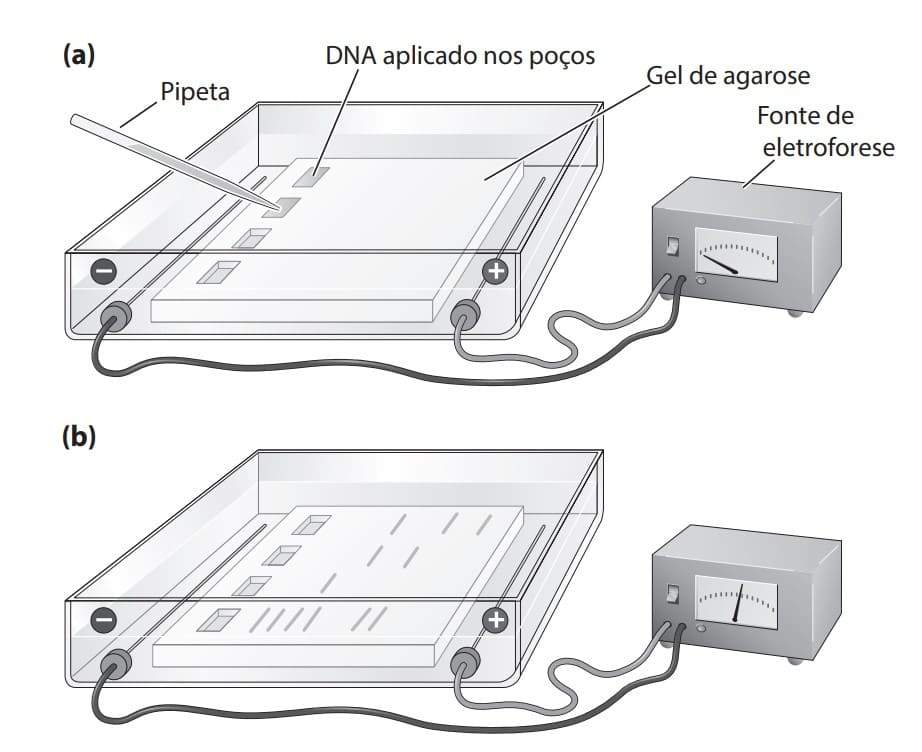
\includegraphics{figures/eletroforese.jpg}

}

\caption{Equipamento utilizado na eletroforese}

}

\end{minipage}%
%
\begin{minipage}[t]{0.50\linewidth}

{\centering 

\raisebox{-\height}{

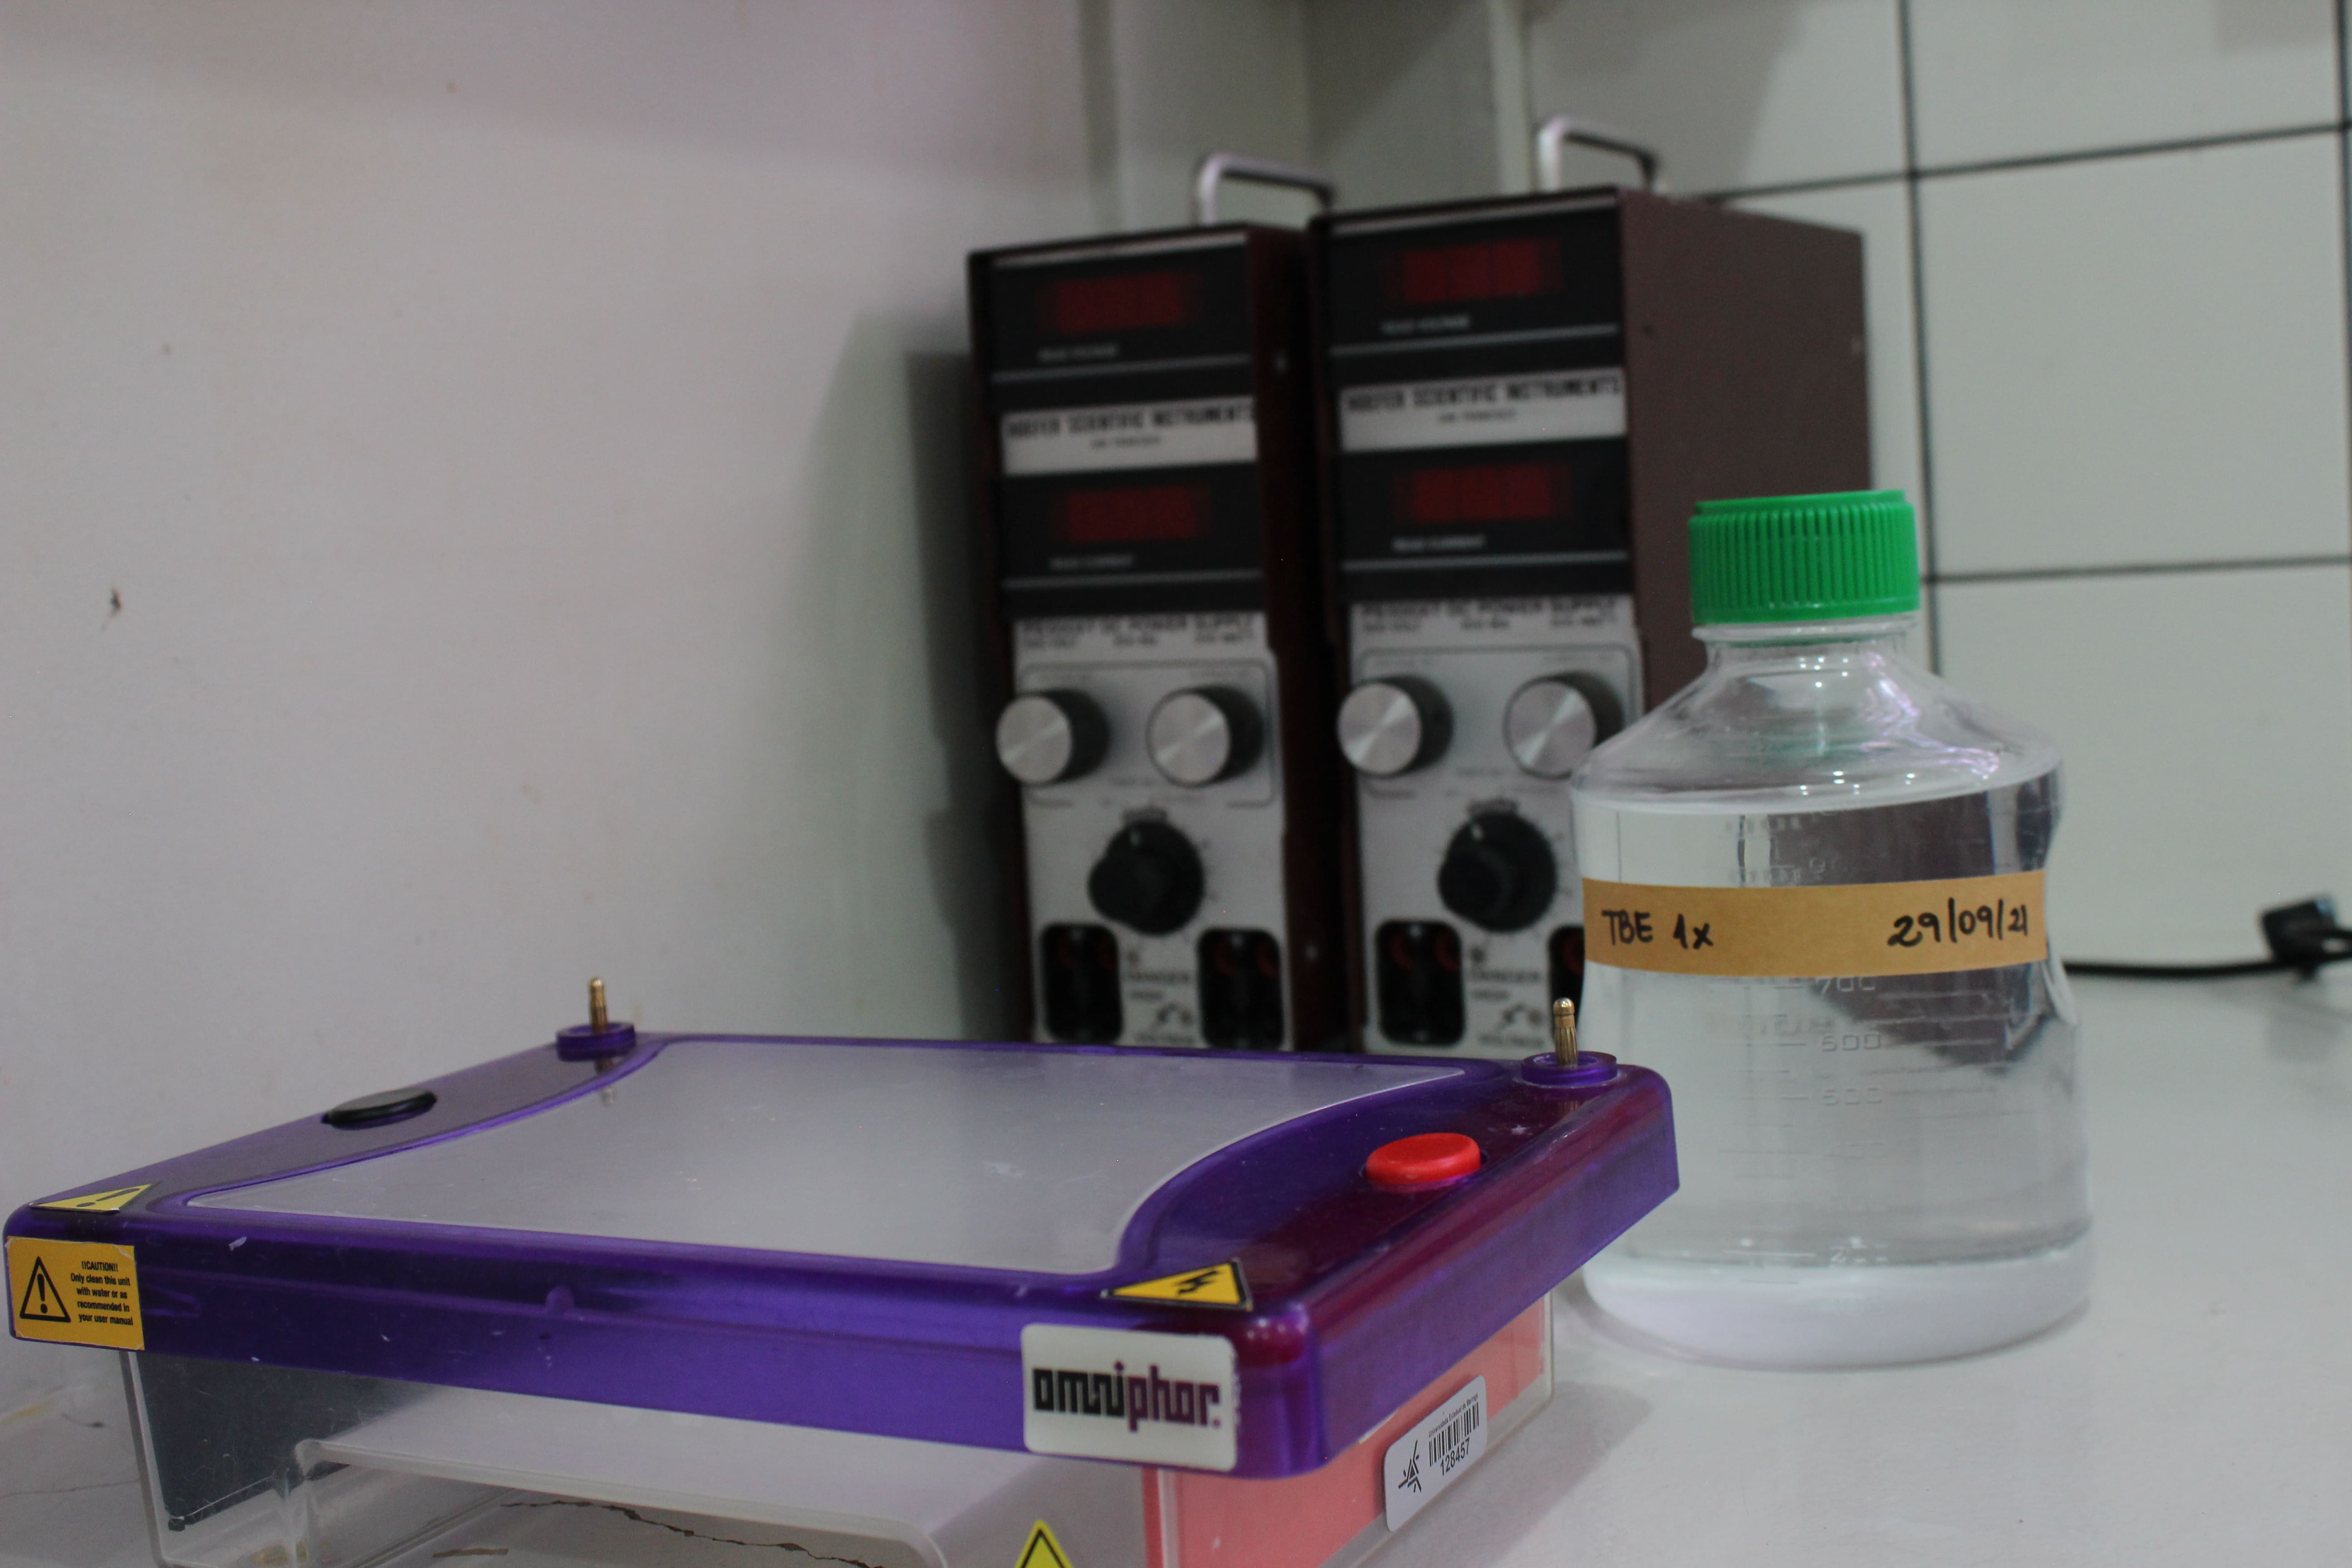
\includegraphics{figures/eletroforese-lab.JPG}

}

\caption{Equipamento do Nupgen}

}

\end{minipage}%

\end{figure}

\hypertarget{ladder}{%
\section{Ladder}\label{ladder}}

O Ladder é um marcador de peso molecular utilizado para determinar o
tamanho dos fragmentos após a amplificação do DNA. É composto por
produtos de PCR e plasmídeos digeridos com enzimas de restrição, sendo
ideal para uso como padrão de peso molecular conhecido para eletroforese
em gel de agarose. O Ladder apresenta bandas de maior intensidade que
irão servir como pontos de referência (geralmente três bandas).

\begin{tcolorbox}[enhanced jigsaw, colback=white, toprule=.15mm, rightrule=.15mm, opacityback=0, left=2mm, arc=.35mm, bottomrule=.15mm, breakable, leftrule=.75mm]
\begin{minipage}[t]{5.5mm}
\textcolor{quarto-callout-note-color}{\faInfo}
\end{minipage}%
\begin{minipage}[t]{\textwidth - 5.5mm}

\textbf{Como fazemos}\vspace{2mm}

No Nupgen há duas opções de Ladder para serem utilizados como padrão, o
Ladder 100 pb e o Ladder 1 Kb. O marcador DNA Ladder 100 pb é o mais
utilizado nos protocolos do laboratório e consiste em múltiplas
repetições de fragmentos de DNA, separados a cada 100 pb até 1 Kb (ou
1400 pb), com fragmentos adicionais de 1500 e 2000 (ou 2072) pb. Já o
marcador de peso molecular DNA Ladder 1 Kb contém 14 fragmentos
facilmente identificáveis, comumente utilizado para a identificação de
massa molecular de fragmentos de DNA entre 250 bp a 10 Kb.

\end{minipage}%
\end{tcolorbox}

\begin{figure}

\begin{minipage}[t]{0.50\linewidth}

{\centering 

\raisebox{-\height}{

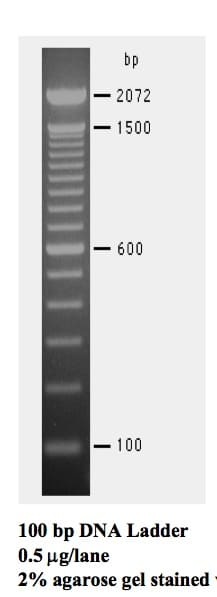
\includegraphics{figures/ladder1000pb.jpg}

}

}

\end{minipage}%
%
\begin{minipage}[t]{0.50\linewidth}

{\centering 

\raisebox{-\height}{

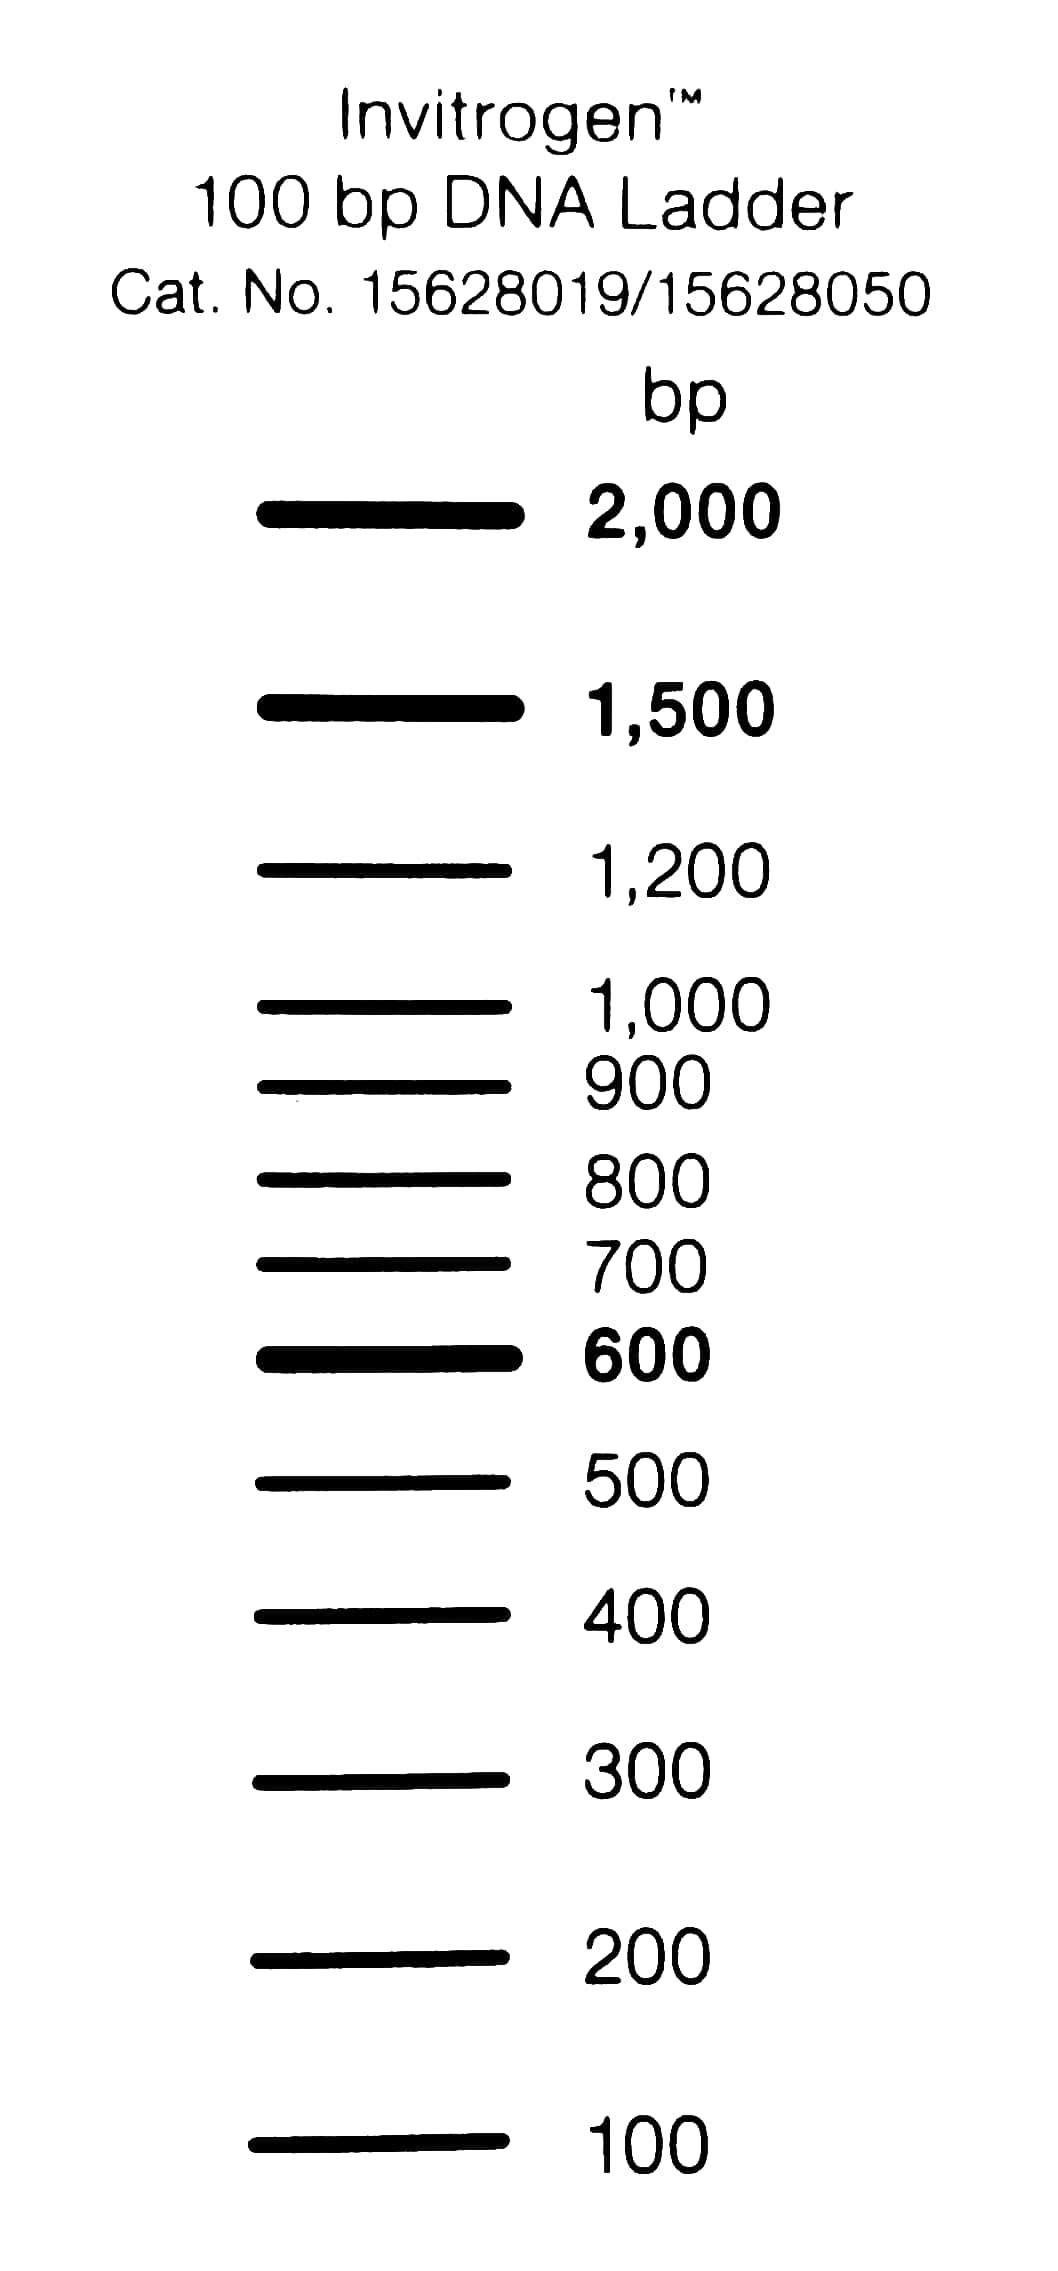
\includegraphics{figures/ladder_100bp_invitrogen.jpeg}

}

}

\end{minipage}%

\end{figure}

\hypertarget{lambda-1}{%
\section{Lambda}\label{lambda-1}}

Lambda é um bacteriófago de \emph{Escherichia coli} e seu DNA contém
48.502 pares de nucleotídeos. É utilizado como DNA padrão com
concentrações conhecidas (por exemplo 5, 10 e 20 ng/μL) para quantificar
o DNA extraído de amostras alvo de estudos por meio da comparação visual
pela fluorescência e espessura das bandas. O DNA fago Lambda é adquirido
de empresas com uma concentração estoque específica e para ser utilizado
na rotina do laboratório é preciso realizar a diluição com base nas
concentrações desejadas.

\begin{tcolorbox}[enhanced jigsaw, colbacktitle=quarto-callout-caution-color!10!white, toprule=.15mm, rightrule=.15mm, opacityback=0, left=2mm, arc=.35mm, breakable, colback=white, bottomtitle=1mm, opacitybacktitle=0.6, toptitle=1mm, leftrule=.75mm, coltitle=black, titlerule=0mm, bottomrule=.15mm, title=\textcolor{quarto-callout-caution-color}{\faFire}\hspace{0.5em}{Cuidado}]

O DNA fago \textbf{Lambda} é utilizado para a quantificação de DNA
extraído em diferentes concentrações, enquanto o \textbf{Ladder} é
utilizado na eletroforese para verificar o tamanho do fragmento de
interesse amplificado após a PCR e nos géis de purificação.

\end{tcolorbox}

\hypertarget{loading}{%
\section{Loading}\label{loading}}

O loading é utilizado para facilitar a visualização da corrida tanto no
momento de aplicação das amostras de DNA no gel, quanto ao final da
corrida através de sua coloração roxa. Além disso, ele possui a função
de aumentar a densidade da amostra, evitando com que ela suba e
trasnforde dos poços durante a corrida do gel. Essa solução é composta
com corante azul de bromofenol e sacarose. Como o DNA não possui cor,
também se adiciona um corante que emite fluorescência para que se
consiga visualizá-lo com clareza no momento em que é exposto à luz UV ou
LED no transiluminador. Os corantes normalmente utilizados são o brometo
de etídio (agente mutagênico e carcinogênico), Saffer e GelRed.

\hypertarget{gel-de-agarose}{%
\section{Gel de agarose}\label{gel-de-agarose}}

O gel de agarose é a matriz na qual é aplicada a amostra e que permite
realizar a separação de moléculas de DNA do polo negativo para o
positivo. A agarose é um polissacarídeo extraído de uma alga marinha
que, quando solidificada, forma uma rede porosa. O tamanho dos poros
dependente da concentração de agarose utilizada para fazer o gel, quanto
maior concentração de agarose menores os poros dificultando a migração
de grandes moléculas de DNA. Essa matriz cria uma resistência, onde
moléculas menores migram mais rápido e moléculas maiores mais devagar. A
capacidade de separar moléculas por tamanho pode ser útil em diversas
aplicações de pesquisa, como por exemplo identificar o tamanho das
amostras desconhecidas em comparação com fragmentos conhecidos.

O gel de agarose deve ser preparado ajustando-se a concentração
apropriada para separar os fragmentos de DNA presentes nas amostras
estudadas. Normalmente, as concentrações de agarose no gel variam de 1\%
a 3\%. Exemplos de dilução serão dadas no tópico a seguir.

\hypertarget{gel-1}\label{gel-1}}

\begin{longtable}[]{@{}l@{}}
\toprule\noalign{}
Cuba - 60 mL \\
\midrule\noalign{}
\endhead
\bottomrule\noalign{}
\endlastfoot
0,6g de agarose \\
12 mL de TBE 5X \\
48 mL de água destilada \\
\end{longtable}

\begin{longtable}[]{@{}l@{}}
\toprule\noalign{}
Cuba - 120 mL \\
\midrule\noalign{}
\endhead
\bottomrule\noalign{}
\endlastfoot
1,2g de agarose \\
24 mL de TBE 5X \\
96 mL de água destilada \\
\end{longtable}

\hypertarget{gel-14}\label{gel-14}}

\begin{longtable}[]{@{}l@{}}
\toprule\noalign{}
Cuba - 120 mL \\
\midrule\noalign{}
\endhead
\bottomrule\noalign{}
\endlastfoot
1,68g de agarose \\
24 mL de TBE 5X \\
96 mL de água destilada \\
\end{longtable}

\hypertarget{gel-3}\label{gel-3}}

\begin{longtable}[]{@{}l@{}}
\toprule\noalign{}
Cuba - 120 mL \\
\midrule\noalign{}
\endhead
\bottomrule\noalign{}
\endlastfoot
3,6g de agarose \\
24 mL de TBE 5X \\
96 mL de água destilada \\
\end{longtable}

\hypertarget{eletroforese-de-amplificauxe7uxe3o-e-purificauxe7uxe3o.}{%
\section{Eletroforese de Amplificação e
Purificação.}\label{eletroforese-de-amplificauxe7uxe3o-e-purificauxe7uxe3o.}}

Obs: O gel para purificação deverá ser novo, enquanto o da amplificação
pode ser reutilizado.

\hypertarget{ladder-100-pb}{%
\subsection{Ladder 100 pb}\label{ladder-100-pb}}

2 μL de loading + 1 μL de GelRed + \textbf{2 μL de Ladder 100 pb}

\hypertarget{por-amostra}{%
\subsection{Por amostra}\label{por-amostra}}

2 μL de loading + 1 μL de GelRed + \textbf{3 μL da PCR}

\begin{tcolorbox}[enhanced jigsaw, colbacktitle=quarto-callout-important-color!10!white, toprule=.15mm, rightrule=.15mm, opacityback=0, left=2mm, arc=.35mm, breakable, colback=white, bottomtitle=1mm, opacitybacktitle=0.6, toptitle=1mm, leftrule=.75mm, coltitle=black, titlerule=0mm, bottomrule=.15mm, title=\textcolor{quarto-callout-important-color}{\faExclamation}\hspace{0.5em}{Importante}]

\begin{itemize}
\tightlist
\item
  Fio preto em cima (polo negativo) e o fio vermelho embaixo (polo
  positivo).
\item
  Gel agarose 1\% (pode ser reutilizado).
\item
  Realizar a corrida eletroforética a 90 volts, por aproximadamente 1
  hora.
\item
  Aplicar o Ladder 100 pb no primeiro poço.
\end{itemize}

\end{tcolorbox}

\hypertarget{eletroforese-de-quantificauxe7uxe3o.}{%
\section{Eletroforese de
Quantificação.}\label{eletroforese-de-quantificauxe7uxe3o.}}

\textbf{Quantificação com gel de agarose}

A eletroforese para quantificação de DNA não é realizada para todos os
organismos trabalhados no laboratório pois em alguns casos (como na
extração de parasitos) a quantidade de DNA extraído é muito pequena para
ser visualizado no gel.

O gel para quantificação deverá ser novo.

Lambda:

\begin{itemize}
\item
  Lambda 5ng/μL - 5μL + 1 μL de GelRed
\item
  Lambda 10ng/μL - 5μL + 1 μL de GelRed
\item
  Lambda 20ng/μL - 5μL + 1 μL de GelRed
\end{itemize}

Amostra - 2 μL de loading + 1 μL de GelRed + 3 μL da PCR

\textbf{Quantificação com Nanodrop}

\hypertarget{quantificauxe7uxe3o}{%
\chapter{Quantificação}\label{quantificauxe7uxe3o}}

Após a etapa de extração, determinar a concentração de DNA, assim como a
sua qualidade e pureza, são fatores importantes para o desenvolvimento
de estudos em biologia molecular. Dessa maneira, as amostras obtidas
podem ser avaliadas quanto à sua concentração e qualidade. Essa
avaliação pode acontecer de algumas maneiras, como realizando uma
\textbf{eletroforese em gel de agarose}, através da \textbf{medição da
absorbância com o uso de espectrofotômetros} ou utilizando
\textbf{fluorímetro} por meio das alterações nas características de
fluorescência na presença de DNA.

A quantificação irá fornecer informações sobre a concentração de DNA
extraído, assim como a integridade das amostras que serão trabalhadas.
Na quantificação utilizando gel de agarose, um gel com concentração de
1\% é preparado e as amostras de DNA são aplicadas juntamente com
amostras de concentrações conhecidas. Para essa finalidade, o DNA do
bacteriófago \textbf{Lambda} é comumente utilizado como padrão. O gel é
normalmente submetido a eletroforese e é realizada uma estimativa visual
através da comparação com o DNA padrão para determinar a concentração de
DNA em cada amostra, analisando a fluorescência e espessura das bandas,
obtendo valores aproximados. Além disso, as amostras consideradas de boa
qualidade irão formar bandas íntegras, enquanto amostras degradadas ou
com presença de moléculas de RNA apresentarão rastros ao longo do gel.

\begin{figure}

{\centering 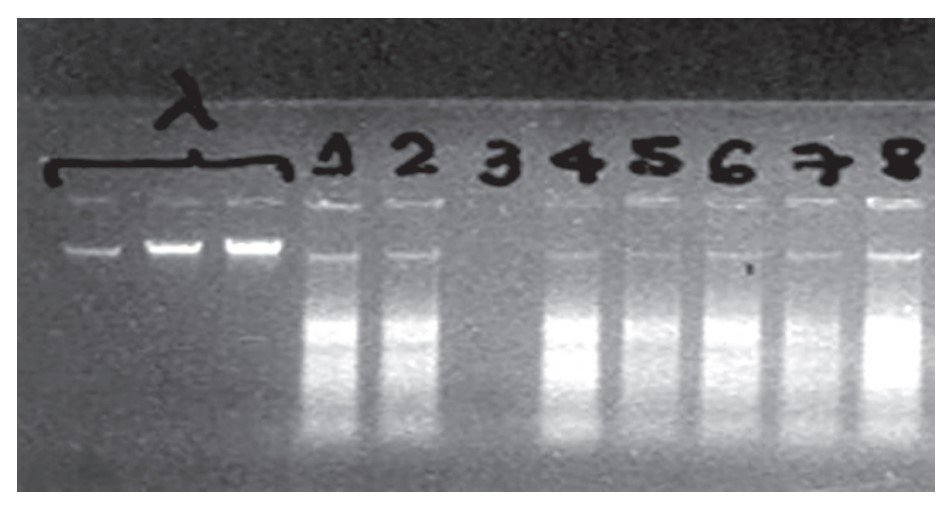
\includegraphics{figures/quantificacao.jpg}

}

\caption{Exemplo de quantificação utilizando gel de agarose e Lambda}

\end{figure}

Por outro lado, a quantificação em espectrofotômetros, como por exemplo
o \textbf{NanoDrop}, fornece dados um pouco mais exatos sobre a
concentração de DNA presente nas amostras. Entretanto, ainda são valores
baseados em um calibrante, tomado como padrão, além de ser necessário
adquirir aparelhos específicos para realizar a quantificação do DNA,
tendo um custo elevado quando comparado à quantificação em gel. Essa
quantificação é baseada na medição da quantidade de luz absorvida pelo
DNA em solução no comprimento de onda de 260 nm. Quanto maior for a
absorção de luz nesse comprimento de onda, maior a concentração de DNA
extraído na amostra.

Já o fluorímetro é um dos métodos mais sensíveis e geralmente utilizado
para amostras com pouca concentração de DNA ou que tenham contaminantes
que absorvem comprimentos de onda de 260 nm. Essa análise acontece pela
luz emitida de moléculas fluorogênicas, sendo um método alternativo para
avaliar a concentração de DNA e RNA marcando a amostra com um marcador
fluorescente (corante fluorescente). Porém, também é um método com um
custo elevado e demanda um tempo maior para preparação das amostras.

\begin{tcolorbox}[enhanced jigsaw, colback=white, toprule=.15mm, rightrule=.15mm, opacityback=0, left=2mm, arc=.35mm, bottomrule=.15mm, breakable, leftrule=.75mm]
\begin{minipage}[t]{5.5mm}
\textcolor{quarto-callout-note-color}{\faInfo}
\end{minipage}%
\begin{minipage}[t]{\textwidth - 5.5mm}

\textbf{Como fazemos}\vspace{2mm}

O método de quantificação geralmente utilizado pelos pesquisadores do
Nupgen é a \textbf{eletroforese em gel de agarose 1\%}, visto que tem
dado certo para a maioria dos grupos trabalhados no laboratório, exceto
parasitas que não passam por essa etapa, indo diretamente para a PCR
devido a baixa concentração de DNA obtida nas amostras. Na quantificação
são utilizadas três concentrações diferentes de DNA Lambda, sendo elas:
5, 10 e 20 ng/μL.

\end{minipage}%
\end{tcolorbox}

A quantificação irá mostrar se as amostras de DNA extraídas precisam ser
\protect\hyperlink{diluiuxe7uxf5es}{diluídas} para a realização da PCR,
pois é preciso ter uma concentração ideal. Dessa forma, quando as
amostras forem quantificadas com valores superiores a 5 ng/μL, elas
precisam ser diluídas. A fórmula utilizada para isso é
\(C1 * V1 = C2 * V2\), onde serão encontradas as quantidades de DNA e
água Milli-Q necessárias para que o DNA fique na concentração final de 5
ng/μL.

\hypertarget{preparauxe7uxe3o-por-amostra}{%
\section{Preparação por amostra}\label{preparauxe7uxe3o-por-amostra}}

\begin{itemize}
\item
  Gel agarose 1\%.
\item
  Correr por aproximadamente 40 minutos, a 100 volts.
\item
  DNA lambda (pipetar 5 μL + 1 μL de GelRed em cada um):

  \begin{itemize}
  \item
    5 ng/μL -- 25 ng
  \item
    10 ng/μL -- 50 ng
  \item
    20 ng/μL -- 100 ng
  \end{itemize}
\end{itemize}

\hypertarget{gelred-1}{%
\subsection{GelRed}\label{gelred-1}}

\textbf{2 μL} de DNA + \textbf{1 μL} de loading + \textbf{1 μL} de
GelRed + \textbf{1 μL} de água Milli-Q\textbf{*}

\textbf{*}água Milli-Q é opcional

\hypertarget{safer}{%
\subsection{Safer}\label{safer}}

\textbf{3 μL} de DNA + \textbf{1 μL} de Safer + \textbf{2 μL} de água
Milli-Q

\hypertarget{diluiuxe7uxe3o-do-dna-para-5ngux3bcl}{%
\section{Diluição do DNA para
5ng/μL}\label{diluiuxe7uxe3o-do-dna-para-5ngux3bcl}}

\(C1 * V1 = C2 * V2\)

\textbf{C1} -- concentração da amostra (inicial)

\textbf{V1} -- quantidade de DNA necessária (descobrir)

\textbf{C2} -- concentração para diluir (vai diluir para 5 ng)

\textbf{V2} -- volume final total (50 μL)

OBS: Quantidade de água Milli-Q é: 50 μL - quantidade de DNA

\hypertarget{amplificauxe7uxe3o}{%
\chapter{Amplificação}\label{amplificauxe7uxe3o}}

Amplificação é o nome dado ao processo de replicação de uma região
específica do DNA alvo de um estudo de modo que seja possível produzir
um grande número de cópias desse mesmo segmento.

A técnica utilizada para a amplificação é a reação em cadeia da
polimerase (\textbf{PCR}), para a execução dessa técnica é preciso
primeiramente fazer a seleção do
\protect\hyperlink{marcadores-moleculares}{marcador molecular} que será
utilizado, ou seja, a região do DNA de interesse a ser replicada, isso
irá variar conforme as necessidades do estudo em questão. Com base nessa
escolha, serão utilizados reagentes específicos com utilidades
diferentes para que a reação aconteça.

\begin{tcolorbox}[enhanced jigsaw, colbacktitle=quarto-callout-tip-color!10!white, toprule=.15mm, rightrule=.15mm, opacityback=0, left=2mm, arc=.35mm, breakable, colback=white, bottomtitle=1mm, opacitybacktitle=0.6, toptitle=1mm, leftrule=.75mm, coltitle=black, titlerule=0mm, bottomrule=.15mm, title=\textcolor{quarto-callout-tip-color}{\faLightbulb}\hspace{0.5em}{Aprendendo}]

Os reagentes utilizados são:

\begin{itemize}
\item
  O \textbf{DNA extraído};
\item
  Um par de oligonucleotídeos iniciadores, os chamados \textbf{primers},
  sendo um \ul{foward} (-\/-\textgreater) e um \ul{reverse}
  (\textless-\/-). Eles irão se ligar na região que deve ser amplificada
  e permitir a ação de uma enzima polimerizadora;
\item
  A enzima DNA polimerase. Normalmente a enzima utilizada nas reações de
  PCR é proveniente da bactéria \emph{\textbf{T}hermus
  \textbf{aq}uaticus} (por isso \textbf{Taq}), uma espécie termófila
  adaptada a viver em águas de alta temperatura, dessa forma, a enzima
  advinda dela é termoestável e consequentemente resistente às altas
  temperaturas da PCR sem sofrer desnaturação;
\item
  Bases nitrogenadas livres, os desoxirribonucleotídeos
  (\textbf{dNTPs});
\item
  Tampão de reação (\textbf{MgCl\textsubscript{2}\textsuperscript{-}}),
  importante para agir como cofator da DNA polimerase;
\item
  Solução \textbf{tampão}, com o objetivo de manter o pH da reação
  estável durante o ciclo de amplificação;
\item
  \textbf{Água Milli-Q}, para completar o volume necessário.
\end{itemize}

\end{tcolorbox}

\begin{figure}

{\centering 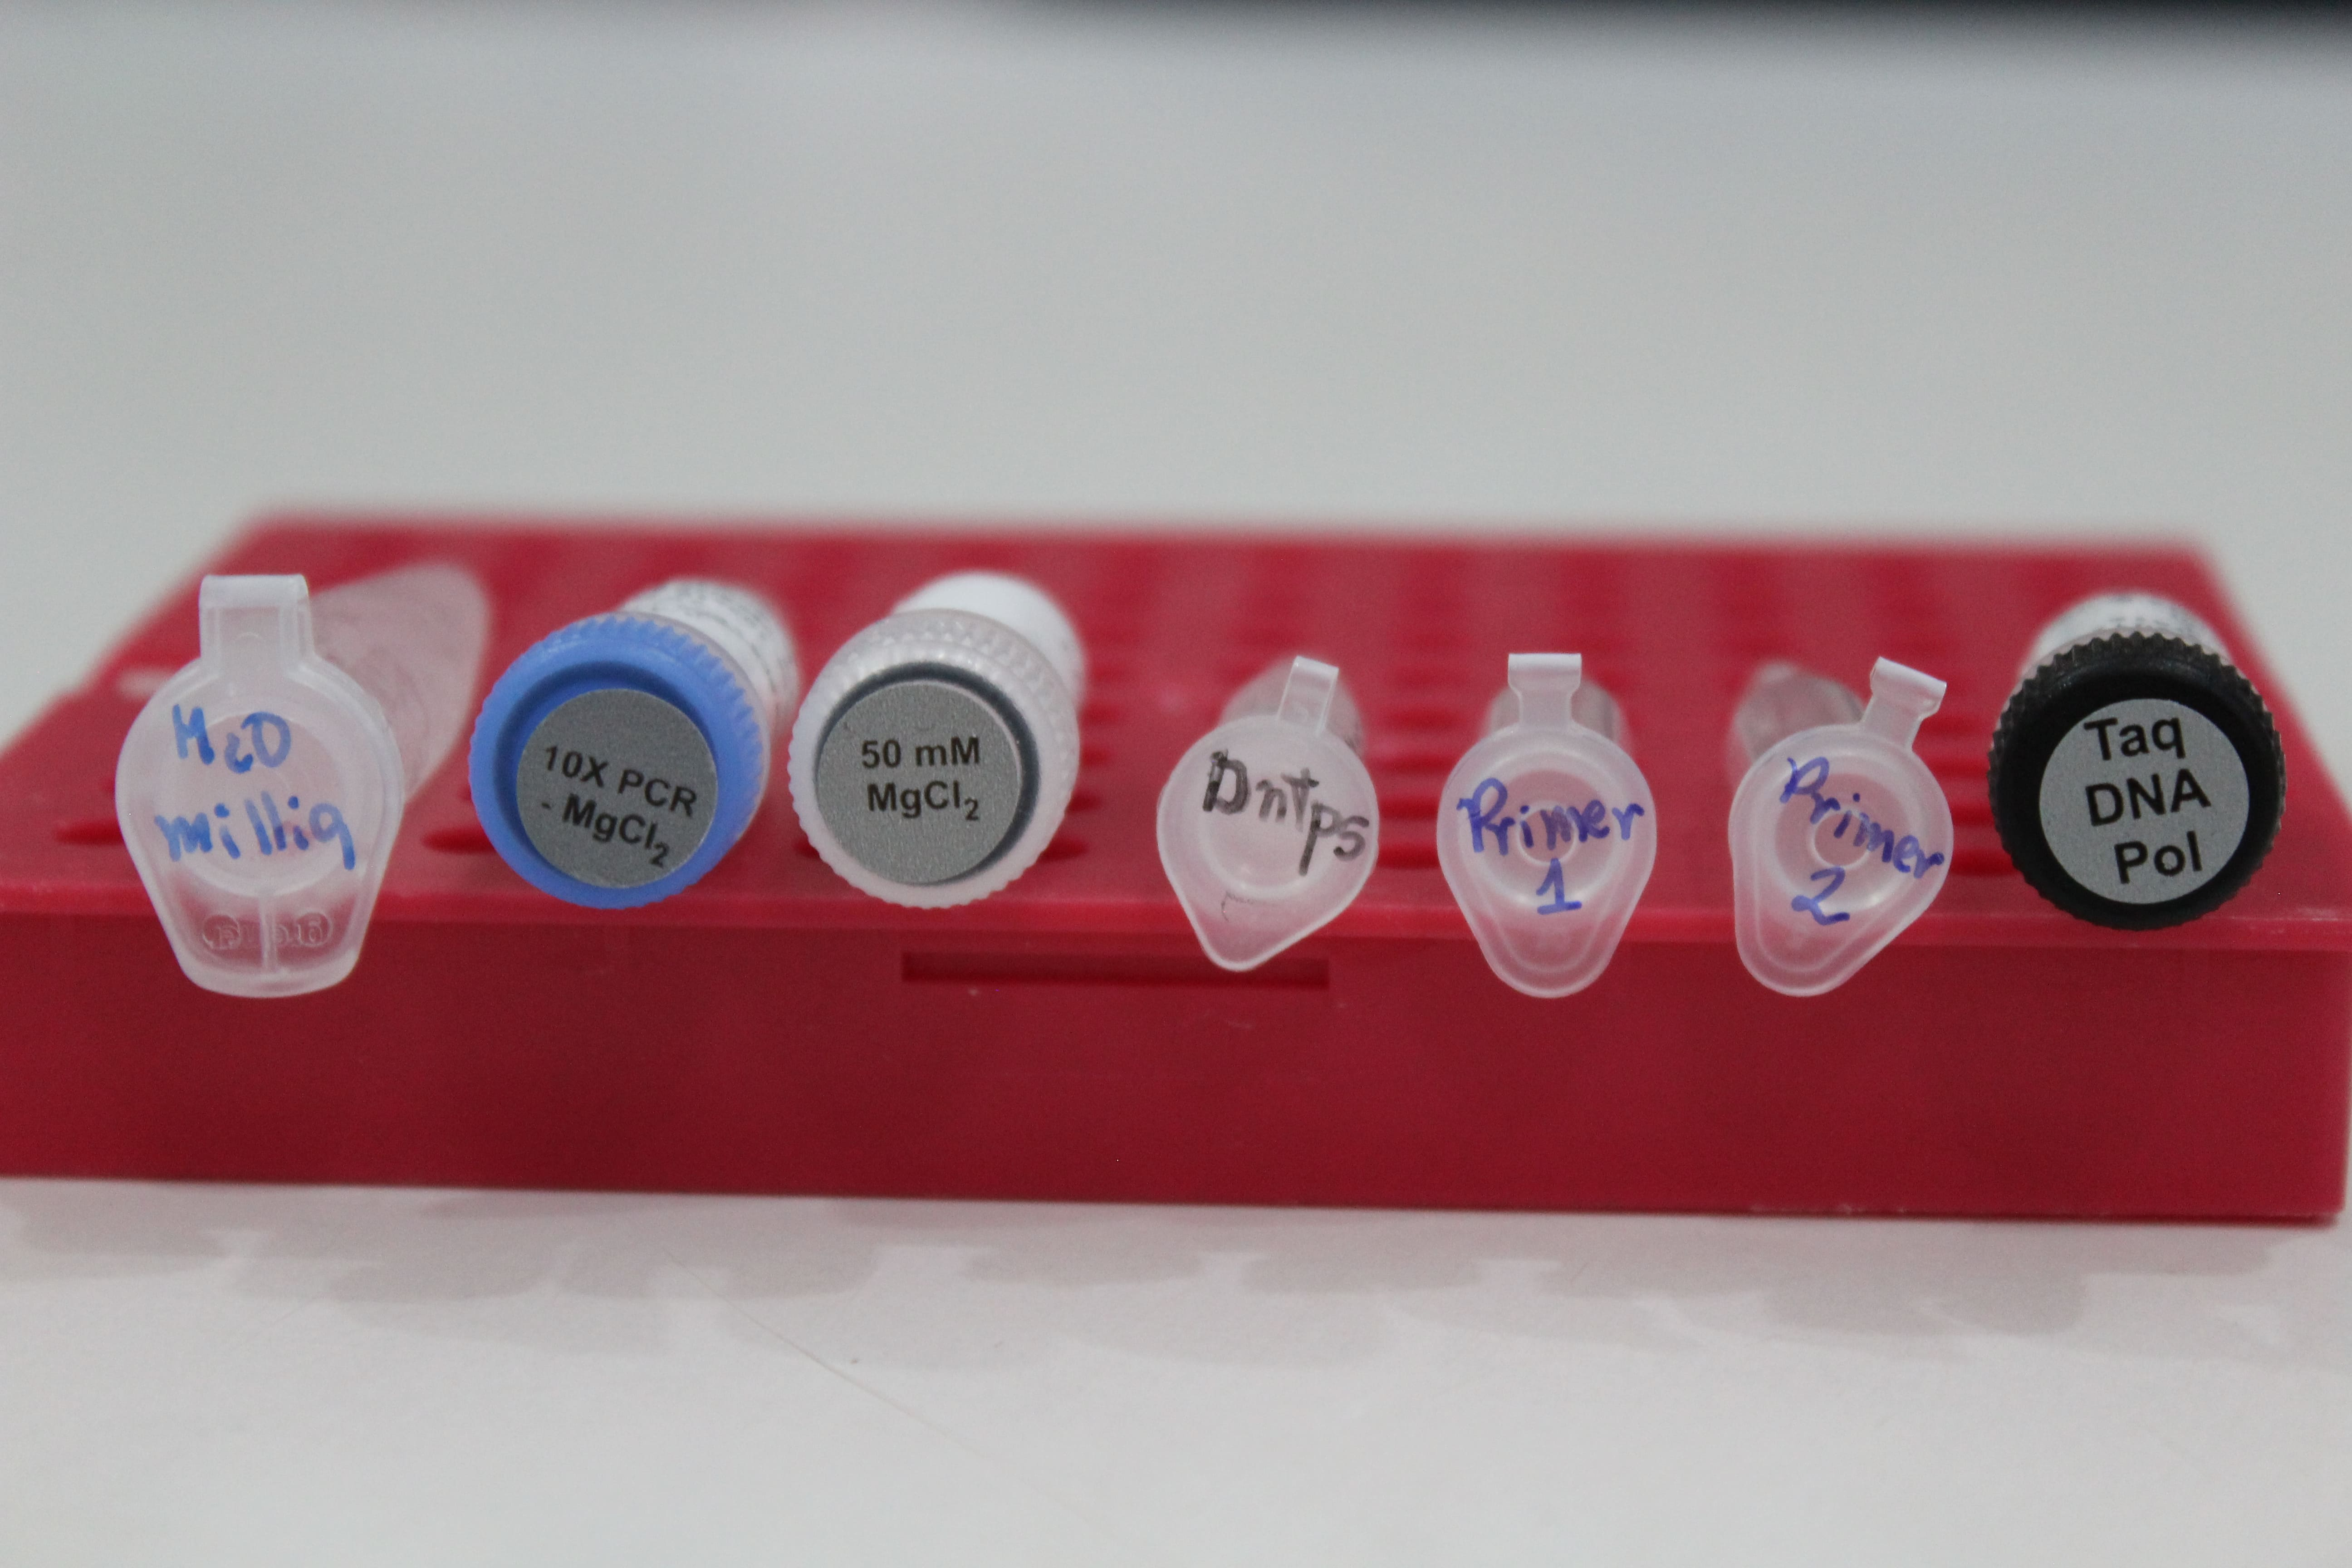
\includegraphics{figures/amplificacao-reagentes.JPG}

}

\caption{Reagentes utilizados na PCR}

\end{figure}

A mistura desses componentes é levada ao termociclador, um aparelho com
a capacidade de aquecer e resfriar as amostras, isso é importante porque
são temperaturas específicas que permitem a abertura das fitas,
anelamento dos primers e a ação da enzima DNA-polimerase. Comumente,
dividimos a PCR em três etapas, são elas:

\begin{enumerate}
\def\labelenumi{\arabic{enumi}.}
\item
  \textbf{Desnaturação:} Nesse momento as fitas de DNA, configuradas em
  dupla-hélice, terão suas ligações de hidrogênio quebradas, sendo assim
  separadas. Essa etapa ocorre graças à elevação da temperatura do
  termociclador a temperaturas acima de 90° C.
\item
  \textbf{Anelamento:} Com as fitas já desnaturadas, a temperatura do
  aparelho é reduzida comumente para valores entre 45° C e 65° C e o par
  de primers, chamados de iniciadores, se ligam com as suas sequências
  complementares na fita molde.
\item
  \textbf{Polimerização:} O termociclador regula a sua temperatura para
  72° C, atingindo a temperatura ótima para a ação da enzima DNA
  polimerase, que começa a síntese de novas fitas utilizando as dNTPs
  livres como matéria prima. A síntese só é possível graças à
  disponibilidade de extremidades 3'OH livres pertencentes aos primers.
\end{enumerate}

As três etapas citadas anteriormente são repetidas em cerca de 20 a 30
ciclos, possibilitando que até bilhões de cópias da região selecionada
sejam produzidas.

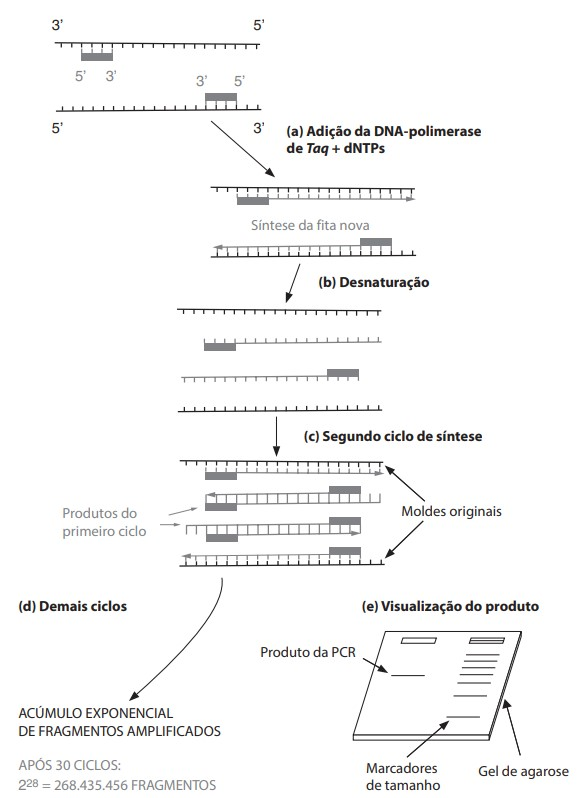
\includegraphics{figures/PCR.jpg}

\hfill\break

\hypertarget{protocolo-de-amplificauxe7uxe3o}{%
\section{\texorpdfstring{\textbf{Protocolo de
amplificação}}{Protocolo de amplificação}}\label{protocolo-de-amplificauxe7uxe3o}}

Para uma reação de PCR iremos precisar de:

\begin{itemize}
\item
  Tubo de 0,5 (novo)
\item
  Tubos de 0,2 (novo)
\item
  Reagentes
\item
  DNA
\item
  Marcador permanente
\end{itemize}

\begin{tcolorbox}[enhanced jigsaw, colback=white, toprule=.15mm, rightrule=.15mm, opacityback=0, left=2mm, arc=.35mm, bottomrule=.15mm, breakable, leftrule=.75mm]
\begin{minipage}[t]{5.5mm}
\textcolor{quarto-callout-note-color}{\faInfo}
\end{minipage}%
\begin{minipage}[t]{\textwidth - 5.5mm}

\textbf{Como fazemos}\vspace{2mm}

\begin{itemize}
\item
  1º Passo: Escrever em cada tubinho de 0,2 o número da amostra
  referente (lembrando de fazer um tubo branco, ou seja, esse é um
  tubinho onde não colocamos DNA, apenas o mix);
\item
  2º Passo: Preparar o mix;
\item
  3º Passo: Distribuir o mix nos tubinhos de 0,2;
\item
  4º Passo: Acrescentar o DNA correspondente em cada tubinho;
\item
  5º Passo: Colocar a reação no termociclador.
\end{itemize}

\end{minipage}%
\end{tcolorbox}

O tubo de 0,5 será utilizado para realizar o mix da PCR. O mix nada mais
é que a junção de todos os reagentes que precisamos em um único tubo
para facilitar na hora de pipetar. Para cada amostra que queremos
realizar PCR com 2μl de DNA, precisa dos seguintes reagentes e
quantidades:

\begin{longtable}[]{@{}ll@{}}
\toprule\noalign{}
\textbf{Reagentes} & \textbf{Quantidade} \\
\midrule\noalign{}
\endhead
\bottomrule\noalign{}
\endlastfoot
Água Milli-Q & 17,50 μL \\
Tampão 10X & 2,50 μL \\
MgCl2 & 1,00 μL \\
dNTPs & 1,00 μL \\
Primer 1 & 0,40 μL \\
Primer 2 & 0,40 μL \\
Taq & 0,20 μL \\
\end{longtable}

\textbf{Obs: Para uma reação com uma quantidade diferente de 2μl de DNA,
o valor alterado para mais ou para menos será sempre da Água Mq.}

Lembrando que para realizar a PCR, é preciso multiplicar o valor da
tabela pelo número de amostras que serão preparadas, somando sempre o
branco e mais uma para margem de erro. Você pode acessar a tabela para
impressão com esses cálculos já realizados no link
\textless\_\_\_\_\_\_\textgreater.

Após realizado o mix, para uma reação de 2μl de DNA, iremos transferir
do tubo do mix 23μl para cada um dos tubinhos de 0,2 (uma reação deve
ter volume total de 25μl). Nesse momento pode utilizar a mesma ponteira,
já que se trata dos mesmos reagentes.

Feito isso, feche o tubo do branco, pois ele já se encontra finalizado e
pode iniciar a distribuição do DNA nos tubinhos de 0,2 respectivos,
lembrando de trocar a ponteira a cada amostra.

\hypertarget{purificauxe7uxe3o}{%
\chapter{Purificação}\label{purificauxe7uxe3o}}

A purificação de DNA após a amplificação é um passo importante na
produção de DNA suficientemente puro para aplicações posteriores, como
sequenciamento ou clonagem. A amplificação do DNA, como a reação em
cadeia da polimerase (PCR), geralmente produz quantidades muito grandes
de DNA, mas também gera muitos contaminantes, como primers, cofator de
PCR e outros produtos de reação. Portanto, é importante purificar o DNA
amplificado antes de usá-lo em outras aplicações.

Existem várias técnicas de purificação de DNA, como centrifugação em
colunas de diálise, precipitação com etanol ou acetato de sódio,
extração com fenol-clorofórmio ou precipitação com polietilenoglicol
(PEG). Cada método tem suas próprias vantagens e desvantagens e o método
ideal dependerá da aplicação específica.

Após confirmar a amplificação do fragmento de interesse, é realizada a
purificação das amostras para remover o excesso de primer, nucleotídeos
e fragmentos de PCR incompletos de baixo peso molecular.

\begin{tcolorbox}[enhanced jigsaw, colback=white, toprule=.15mm, rightrule=.15mm, opacityback=0, left=2mm, arc=.35mm, bottomrule=.15mm, breakable, leftrule=.75mm]
\begin{minipage}[t]{5.5mm}
\textcolor{quarto-callout-note-color}{\faInfo}
\end{minipage}%
\begin{minipage}[t]{\textwidth - 5.5mm}

\textbf{Como fazemos}\vspace{2mm}

No Nupgen, essa purificação é realizada por meio de uma etapa de
precipitação com polietilenoglicol (PEG), protocolo descrito a princípio
por Rosenthal, Coutelle, e Craxton (1993) . A mistura de PEG precipita
seletivamente DNA de 100 bp a 150 pb, deixando primers residuais,
nucleotídeos e produtos de PCR incompletos no sobrenadante. Dessa
maneira, o sobrenadante é removido, ficando precipitado apenas o DNA
amplificado.

\end{minipage}%
\end{tcolorbox}

Por fim, é feita uma eletroforese em gel de agarose para verificar se a
purificação foi bem-sucedida e se as amostras podem ser utilizadas para
o sequenciamento.

\begin{figure}

{\centering 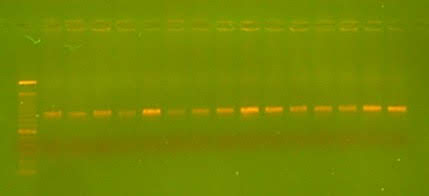
\includegraphics{gel_purificacao.jpg}

}

\caption{Foto de um gel de purificação}

\end{figure}

\hypertarget{purificauxe7uxe3o-com-polietilenoglicol-peg}{%
\section{Purificação com Polietilenoglicol
(PEG)}\label{purificauxe7uxe3o-com-polietilenoglicol-peg}}

\begin{enumerate}
\def\labelenumi{\arabic{enumi}.}
\item
  Adicionar 50 μL de PEG 20\% NaCl 25m. em um tubo de 1,5 mL.
\item
  Transferir a PCR para o tubo e misturar.
\item
  Incubar o conteúdo do tubo a 37oC por 15 minutos.
\item
  Centrifugar a reação + PEG por 15 minutos a 12000 rpm.
\item
  Retirar o sobrenadante sem tocar na parede do tubo e descartar -- usar
  pipeta.
\item
  Adicionar 62,5 μL de etanol 80\% (álcool Merck) gelado no tubo --
  colocar na parede.
\item
  Centrifugar por 2 minutos.
\item
  Virar o tubo, descartando o sobrenadante.
\item
  Deixar secar até não ter mais gotas -- pode ser na estufa.
\item
  Ressuspender com 10 μL de água Milli-Q lavando a parede do tubo de 5 a
  6 vezes.
\end{enumerate}

\hypertarget{sequenciamento}{%
\chapter{Sequenciamento}\label{sequenciamento}}

Depois de realizada a purificação, o fragmento purificado pode ser
sequenciado. O sequenciamento de DNA consiste no processo de
determinação da sequência de nucleotídeos (\textbf{A, T, G e C}) em um
fragmento de DNA. A informação contida nessas sequências de nucleotídeos
possibilita diversos tipos de aplicações, como, por exemplo, identificar
o organismo ao qual pertence uma amostra, diagnosticar uma doença
genética, aplicar em estudos de filogenia e diversidade genética, entre
outros.

\begin{tcolorbox}[enhanced jigsaw, colbacktitle=quarto-callout-tip-color!10!white, toprule=.15mm, rightrule=.15mm, opacityback=0, left=2mm, arc=.35mm, breakable, colback=white, bottomtitle=1mm, opacitybacktitle=0.6, toptitle=1mm, leftrule=.75mm, coltitle=black, titlerule=0mm, bottomrule=.15mm, title=\textcolor{quarto-callout-tip-color}{\faLightbulb}\hspace{0.5em}{Aprendendo}]

Existem vários métodos para o sequenciamento do DNA, tais como:

\begin{itemize}
\item
  O método enzimático (\textbf{1ª Geração}) de Frederik Sanger (1980);
\item
  O método de pirosequenciamento (\textbf{2ª Geração}) de Mostafa
  Ronaghi (1996);
\item
  O de \textbf{3ª Geração}, Single Molecule Real Time (SMRT) - DNA
  Sequencing;
\item
  Métodos mais modernos conhecidos como \textbf{Sequenciamento de Nova
  Geração (NGS)}.
\end{itemize}

\end{tcolorbox}

A técnica desenvolvida por Sanger e colaboradores possibilitou a
determinação da sequência nucleotídica e se tornou mais acessível devido
aos avanços recentes na fabricação de equipamentos automatizados. Além
disso, é um dos métodos mais utilizados (inclusive nos trabalhos do
Nupgen) e consiste na adição de um reagente único: \textbf{os
didesoxirribonucleotídeos trifosfatados (ddNTPs)}. É realizada uma
reação de sequenciamento, contendo os mesmos reagentes utilizados na
\protect\hyperlink{amplificauxe7uxe3o}{Reação em Cadeia da Polimerase},
com a presença dos ddNTPS, ou seja, terminadores de cadeia para os
quatro nucleotídeos (\textbf{ddATP, ddTTP, ddCTP, ddGTP}), cada um deles
marcado com um corante fluorescente de cores diferentes.

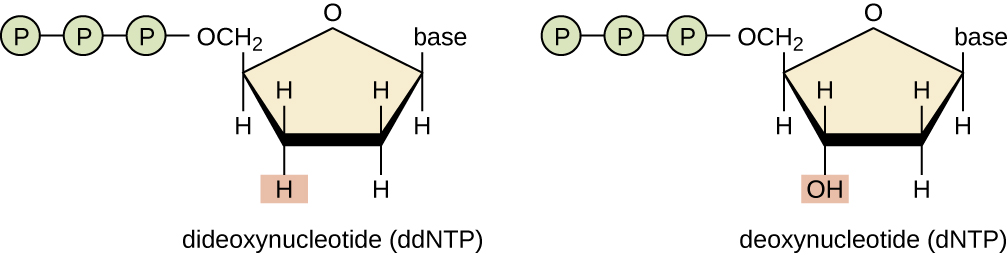
\includegraphics{figures/ddNTPs.jpg}

A variação no tamanho dos fragmentos acontece por essa adição de
nucleotídeos modificados (ddNTPs) juntamente com nucleotídeos normais
(dNTPs). Os ddNTPS não possuem o radical hidroxila (OH) no carbono 3' da
ribose, então ao serem incorporados na fita que está sendo sintetizada,
haverá a interrupção dessa síntese. É uma adição aleatória e produzirá
fragmentos terminados em cada uma das posições dos nucleotídeos da
sequência de DNA que se deseja analisar. Dessa maneira, o método de
Sanger consiste na produção de fragmentos de DNA com tamanhos que
diferem em um nucleotídeo, utilizando como molde uma fita simples de
DNA.

\begin{figure}

\begin{minipage}[t]{0.50\linewidth}

{\centering 

\raisebox{-\height}{

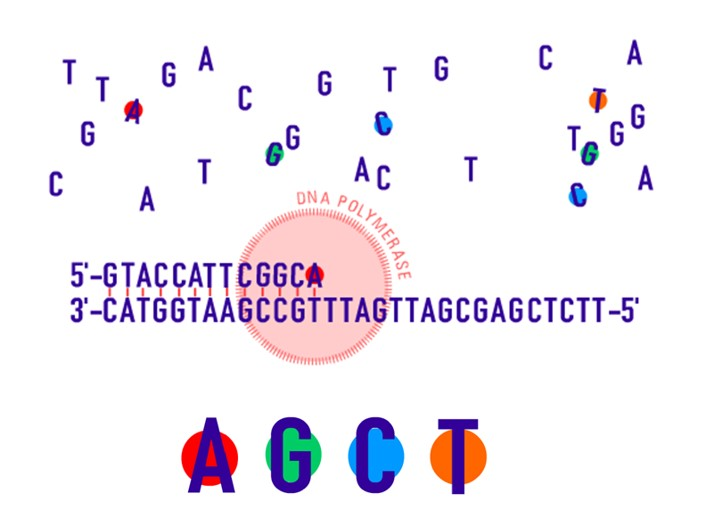
\includegraphics{figures/Seq1.jpg}

}

}

\end{minipage}%
%
\begin{minipage}[t]{0.50\linewidth}

{\centering 

\raisebox{-\height}{

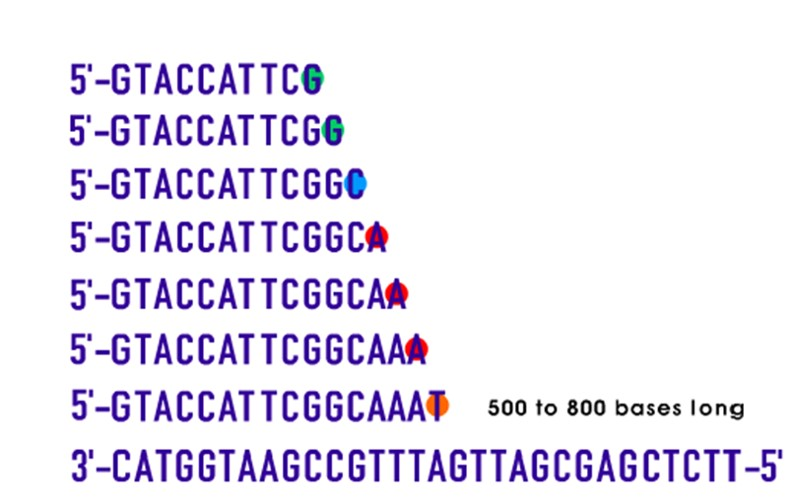
\includegraphics{figures/Seq2.jpg}

}

}

\end{minipage}%

\end{figure}

Os equipamentos automatizados utilizados hoje em dia para o
sequenciamento possuem capilares extremamente finos que por meio da
migração por eletroforese capilar, irão alinhar os fragmentos com base
em seu tamanho (do menor para o maior), detectando por um feixe de laser
a marcação de cada um dos quatro ddNTPs com a molécula fluorescente.
Isso permite identificar qual foi o nucleotídeo adicionado em cada
posição terminal dos fragmentos, construindo a sequência da molécula de
DNA alvo dos estudos. Essa técnica é geralmente utilizada para o
sequenciamento de moléculas com aproximadamente 100 e 1000 pb. Como
resultado do sequenciamento, são obtidos os \textbf{eletroferogramas},
que apresentam picos representando cada um dos nucleotídeos e
consequentemente a sequência do fragmento de interesse.

\begin{figure}

\begin{minipage}[t]{\linewidth}

{\centering 

\raisebox{-\height}{

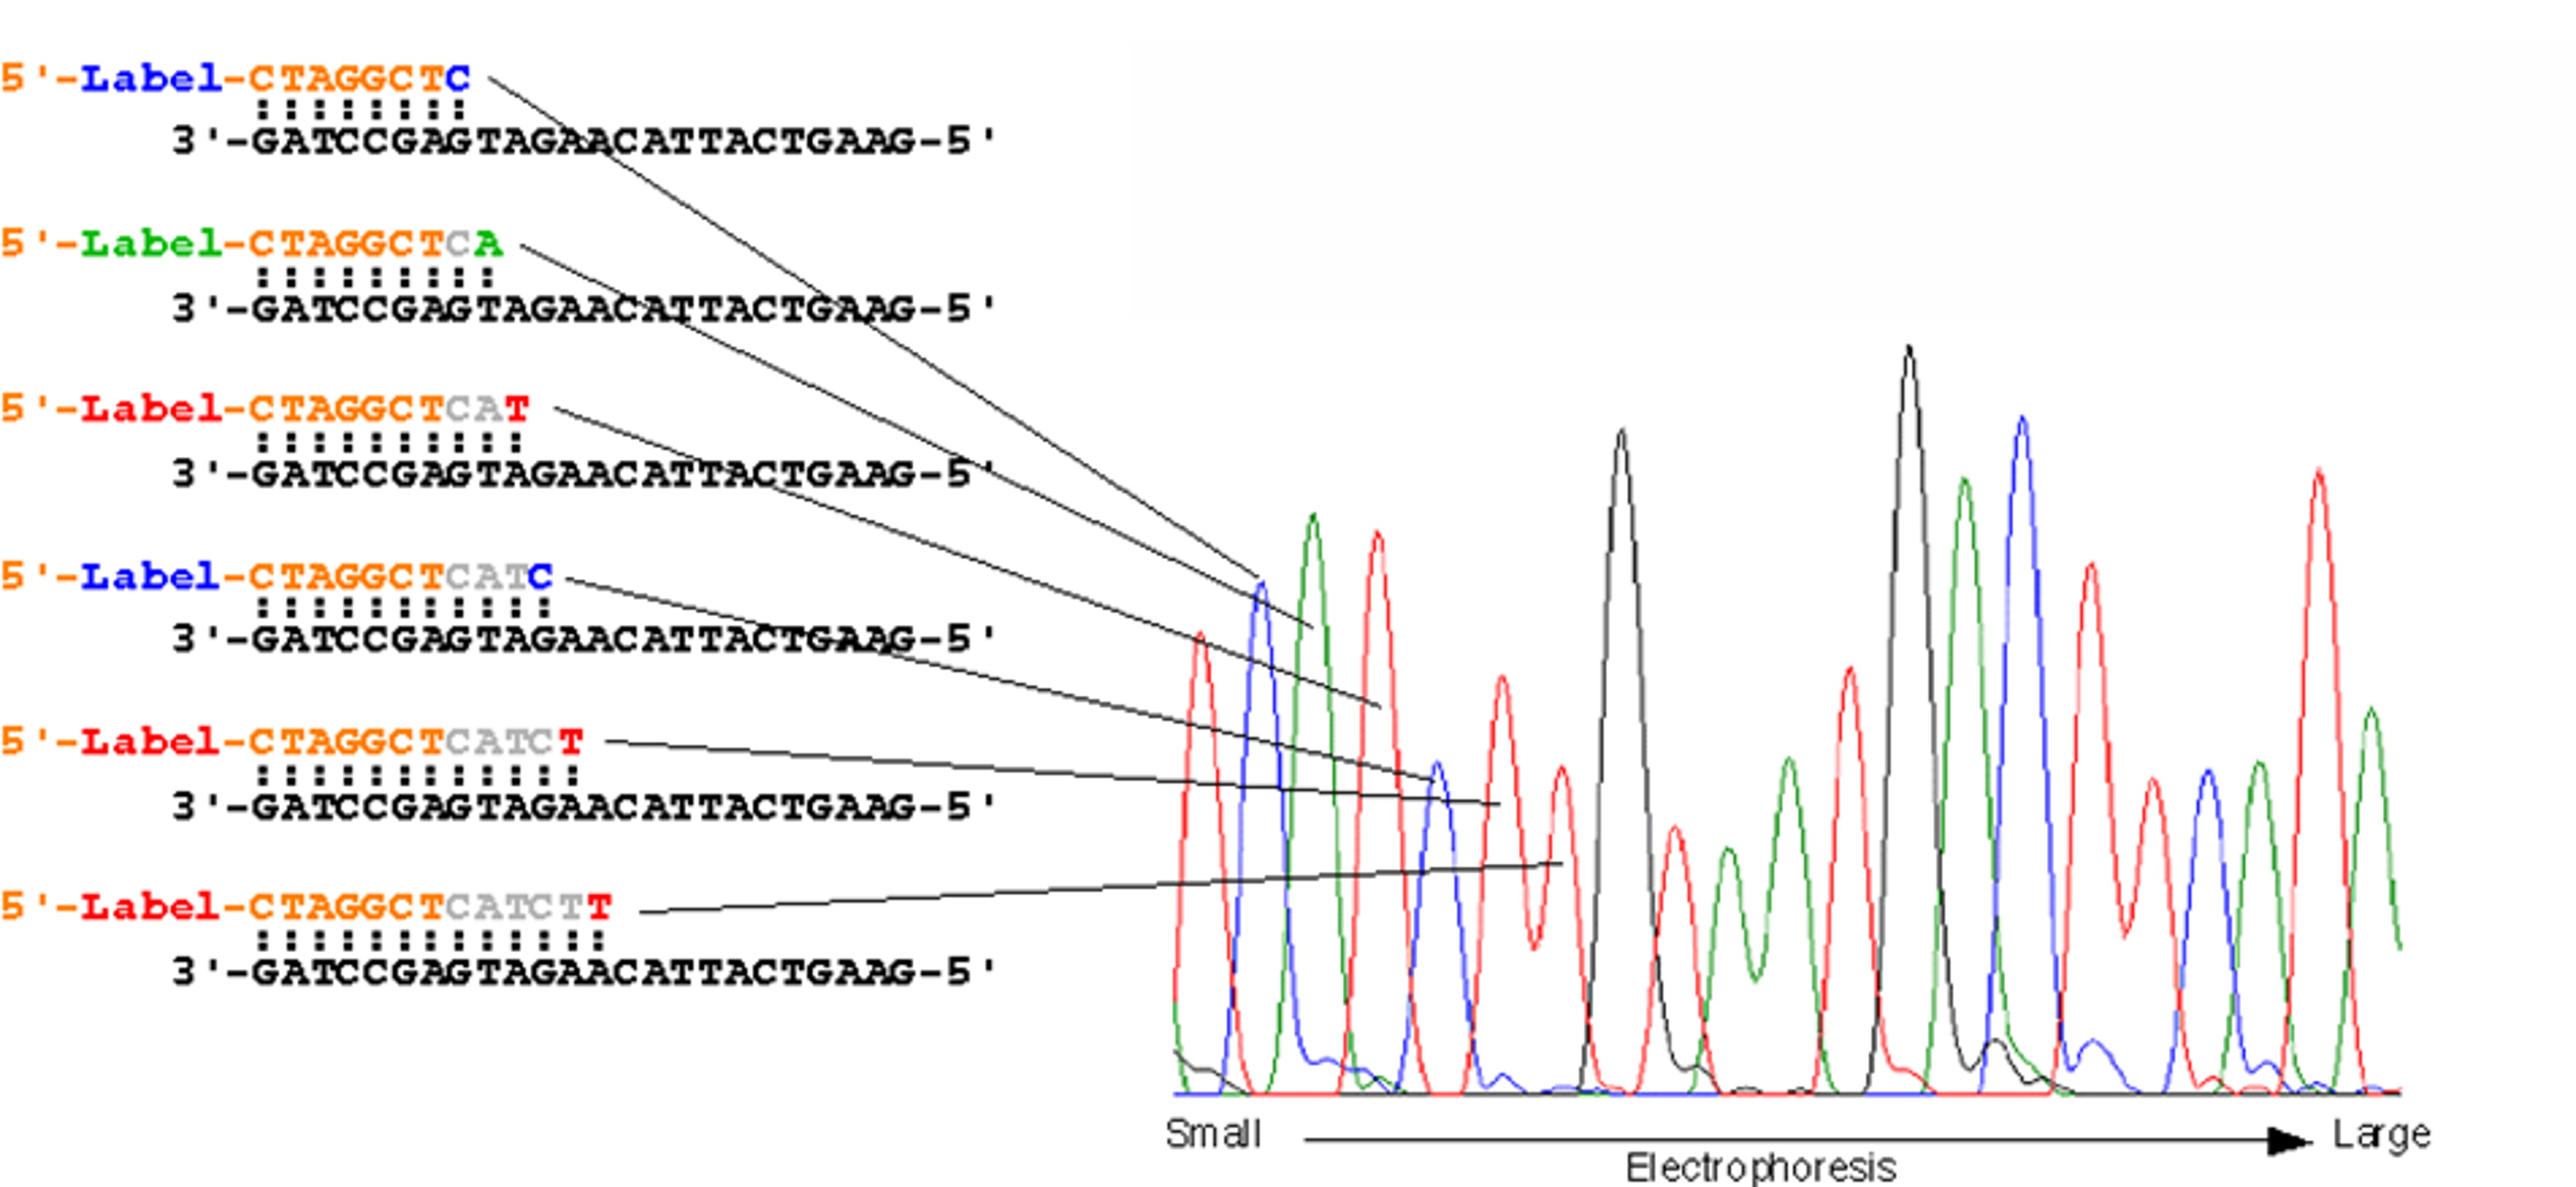
\includegraphics{figures/eletroferograma.jpg}

}

\caption{Eletroferograma}

}

\end{minipage}%

\end{figure}

\begin{tcolorbox}[enhanced jigsaw, colback=white, toprule=.15mm, rightrule=.15mm, opacityback=0, left=2mm, arc=.35mm, bottomrule=.15mm, breakable, leftrule=.75mm]
\begin{minipage}[t]{5.5mm}
\textcolor{quarto-callout-note-color}{\faInfo}
\end{minipage}%
\begin{minipage}[t]{\textwidth - 5.5mm}

\textbf{Como fazemos}\vspace{2mm}

Atualmente, o Nupgen envia as amostras para o sequenciamento para a
empresa ACTGene Análises Moleculares LTDA que utilizada o sequenciador
automatizado Applied Biosystems® AB 3500 Genetic Analyzer
(sequenciamento de Sanger). Essa empresa é do Rio Grande do Sul, então
as amostras são preparadas e devidamente acondicionadas para serem
enviadas pelos correios.

Site da ACTGene: \url{https://actgene.com.br/}

Informações sobre envio/preparo das amostras:
\url{https://actgene.com.br/wp-content/uploads/2022/06/ACTGene_Guia-preparo-de-amostras.pdf}

\end{minipage}%
\end{tcolorbox}

\part{Análises}

\hypertarget{bancos-de-dados-genuxe9ticos}{%
\chapter{Bancos de Dados Genéticos}\label{bancos-de-dados-genuxe9ticos}}

\hypertarget{genbank}{%
\section{GenBank}\label{genbank}}

\textbf{Link: \href{}{https://www.ncbi.nlm.nih.gov/genbank/}}

O GenBank é um banco de dados de sequências de DNA mantido pelo National
Center for Biotechnology Information (NCBI), um instituto do National
Institutes of Health (NIH) dos Estados Unidos. Ele armazena sequências
de DNA de diversas fontes, incluindo genomas, sequências de expressão
gênica, sequências de proteínas e etc.

O GenBank é um recurso valioso para os pesquisadores de genética
molecular porque permite o acesso a uma ampla variedade de sequências de
DNA, tornando mais fácil a realização de análises e pesquisas. Além
disso, o GenBank permite a submissão de novas sequências de DNA pelos
usuários, o que permite o compartilhamento de dados entre os
pesquisadores.

Todo trabalho ao ser publicado deve submeter as sequências utilizadas
para o GenBank, dessa forma outros pesquisadores podem utilizar em suas
próprias análises.

\hypertarget{bold-systems}{%
\section{BOLD Systems}\label{bold-systems}}

\textbf{Link: \href{}{http://boldsystems.org/}}

O BOLD Systems (Barcode of Life Data Systems) é um projeto de ciência
cidadã que visa coletar e armazenar sequências de DNA barcodes
(\protect\hyperlink{marcadores-moleculares}{COI}) de espécies de todo o
mundo. O DNA barcode é um trecho curto de DNA que pode ser usado para
identificar espécies de maneira rápida e precisa. Ele é amplamente
utilizado em biologia evolutiva e conservação de espécies e é uma
ferramenta valiosa para a identificação de espécies em ambientes
complexos, como ecossistemas tropicais.

O BOLD Systems é mantido pelo Instituto de Biodiversidade do Canadá e é
uma iniciativa internacional que conta com a participação de cientistas,
conservacionistas e cidadãos do mundo todo. Ele possui uma base de dados
online que armazena as sequências de DNA barcodes coletadas e permite o
acesso a essas sequências pelos usuários.

\hypertarget{blast}{%
\section{BLAST}\label{blast}}

\textbf{Link: \href{}{https://blast.ncbi.nlm.nih.gov/Blast.cgi}}

O BLAST (Basic Local Alignment Search Tool) é uma ferramenta amplamente
utilizada pelos pesquisadores de genética molecular para realizar buscas
de sequências de DNA em bancos de dados de sequências. Ele é mantido
pelo National Center for Biotechnology Information (NCBI) e está
disponível gratuitamente na internet.

O BLAST funciona comparando uma sequência de entrada com as sequências
armazenadas em um banco de dados de referência e encontrando as
sequências mais similares. Ele utiliza uma técnica de alinhamento de
sequências chamada alinhamento local, que permite o alinhamento apenas
de trechos similares das sequências, ignorando trechos com pouca
similaridade.

O BLAST é amplamente utilizado em diversas análises de genética
molecular, como a identificação de genes e/ou espécies.

\hypertarget{softwares}{%
\chapter{Softwares}\label{softwares}}

Em nosso laboratório dependemos bastante do uso de diversos softwares
para realizar diferentes análises. Enquanto o início dos trabalhos é
feito com aparelhos em nosso laboratório, após receber os resultados do
sequenciamento, dependemos de análises realizadas no próprio computador.

Para isso, precisamos entender como as análises funcionam e também qual
a melhor forma que realizá-las, evitando dores de cabeça por resultados
que não refletem a realidade.

A seguir vamos apresentar os principais softwares utilizados, bem como
algumas dicas que podem facilitar o trabalho. Lembre-se, é muito mais
fácil aprender com outros alunos do que apenas com os manuais de cada
programa. Peça ajuda, principalmente com as análises, que podem gerar
resultados errados e atrapalhar toda sua pesquisa.

\hypertarget{bioedit}{%
\section{BioEdit}\label{bioedit}}

\textbf{Útil para: {Edição}}

BioEdit é um editor de sequências de DNA e proteínas muito utilizado na
genética molecular. Ele é especialmente útil na visualização de
eletroferogramas, que são gráficos gerados por sequenciadores de DNA que
mostram a sequência de base de uma amostra de DNA.

O BioEdit permite a visualização de eletroferogramas de maneira fácil e
rápida, além de fornecer uma ampla gama de ferramentas para análise de
sequências, como alinhamento de sequências, análise de substituição de
nucleotídeos e proteínas, e muito mais. Ele também possui uma interface
intuitiva e é compatível com Windows, MacOS e Linux.

Além da visualização de eletroferogramas, o BioEdit é amplamente
utilizado em diversas outras tarefas de genética molecular, como edição
de sequências, anotação de genes e análise de expressão gênica.

Usos

\textbf{Prós}

\textbf{Contras}

\begin{itemize}
\tightlist
\item
  A última versão disponível é de 2005.
\end{itemize}

\hypertarget{mega}{%
\section{MEGA}\label{mega}}

\textbf{Útil para: {Edição} / {Alinhamento} / {Modelo} / {Árvore}}

O MEGA (Molecular Evolutionary Genetics Analysis) é um software de
análise de genética molecular utilizado para estudar a evolução e a
relação filogenética entre sequências de DNA, RNA ou proteínas. Ele é
amplamente utilizado por pesquisadores em diversas áreas da genética
molecular, incluindo biologia evolutiva, genômica e epidemiologia de
doenças.

O MEGA possui uma ampla gama de recursos, incluindo alinhamento de
sequências, inferência de árvores filogenéticas, análise de substituição
de nucleotídeos e proteínas, e muito mais. Ele também permite a
visualização e análise de dados de diversas maneiras, como gráficos e
tabelas.

Ele um software fácil de usar, com uma interface intuitiva e uma ampla
base de usuários e recursos on-line disponíveis. Ele é compatível com
Windows, MacOS e Linux e está disponível para download gratuito em seu
site oficial.

\begin{tcolorbox}[enhanced jigsaw, colbacktitle=quarto-callout-warning-color!10!white, toprule=.15mm, rightrule=.15mm, opacityback=0, left=2mm, arc=.35mm, breakable, colback=white, bottomtitle=1mm, opacitybacktitle=0.6, toptitle=1mm, leftrule=.75mm, coltitle=black, titlerule=0mm, bottomrule=.15mm, title=\textcolor{quarto-callout-warning-color}{\faExclamationTriangle}\hspace{0.5em}{Aviso}]

Atualmente o MEGA está na versão \textbf{11}, mas contém um ou outro bug
que pode atrapalhar bastante. O MEGA \textbf{7} possui quase todas as
ferramentas que precisamos e é mais estável. Recomendamos usar essa
versão para coisas básicas.

\end{tcolorbox}

Usos

\textbf{Prós}

\begin{itemize}
\tightlist
\item
  É simples e fácil de aprender.
\end{itemize}

\textbf{Contras}

\begin{itemize}
\tightlist
\item
  Roda no computador e algumas análises (como árvores ML) podem ser bem
  demoradas.
\end{itemize}

\hypertarget{iqtree}{%
\section{IQTree}\label{iqtree}}

\textbf{Útil para: {Modelo} / {Árvore}}

Usos

\textbf{Prós}

\textbf{Contras}

\hypertarget{jmodeltest}{%
\section{jModelTest}\label{jmodeltest}}

\textbf{Útil para: {Modelo}}

Usos

\textbf{Prós}

\begin{itemize}
\tightlist
\item
  Bastante reconhecido e utilizado em outros trabalhos.
\end{itemize}

\textbf{Contras}

\begin{itemize}
\tightlist
\item
  É bem demorado.
\end{itemize}

\hypertarget{raxml}{%
\section{RAxML}\label{raxml}}

\textbf{Útil para: {Árvore}}

\textbf{Link: \url{https://raxml-ng.vital-it.ch}}

RAxML (Randomized Axelerated Maximum Likelihood) é um software de
análise filogenética utilizado para inferir árvores filogenéticas a
partir de sequências de DNA, RNA ou proteínas. Ele é especialmente útil
para análises com grandes conjuntos de dados, pois é capaz de processar
grandes quantidades de dados de maneira rápida e eficiente.

O RAxML possui vários métodos de inferência de árvores filogenéticas,
como o método de máxima verossimilhança (ML) e o método de Bayesiano.
Ele também permite a realização de análises bootstrap, que são usadas
para avaliar a confiabilidade das árvores filogenéticas inferidas.

\textbf{Prós}

\begin{itemize}
\item
  Fácil uso;
\item
  Não requer uso de memória do computador, ele roda em servidor.
\end{itemize}

\textbf{Contras}

\begin{itemize}
\tightlist
\item
  Tem um limite de bootstrap de 100
\end{itemize}

\hypertarget{phyml}{%
\section{PhyML}\label{phyml}}

\textbf{Útil para: {Modelo} / {Árvore}}

\textbf{Link: \url{http://www.atgc-montpellier.fr/phyml/}}

Phylogenetic Maximum Likelihood (PhyML) é um servidor online para gerar
inferências filogenéticas pelo método de máxima verossimilhança. O
servidor é intuitivo, portanto, de fácil uso. Para gerar uma árvore
filogenética no PhyML, é preciso fornecer um arquivo de alinhamento no
formato PHYLIP (é possível exportar alinhamentos neste formato na versão
do MEGA \textbf{10}). Após o término das análises, o PhyML fornece um
arquivo zip que contém, além da árvore, outros relatórios estatísticos
(como a lista dos modelos evolutivos, por exemplo)

\textbf{Prós:}

\begin{itemize}
\item
  Fácil uso;
\item
  Permite realizar várias customizações nos parâmetros estatísticos que
  não são possíveis de personalizar em outros softwares, como o MEGA;
\item
  Possui bootstrap de 1000;
\item
  Não requer uso de memória do computador, ele roda em servidor.
\end{itemize}

\textbf{Contras:}

\begin{itemize}
\item
  Utiliza o formato PHYLIP, diferente de outros que utilizam FASTA, por
  isso é possível que o usuário tenha que formatar os terminais da
  árvore, um trabalho manual desgastante. Recomendamos o uso do pacote
  \protect\hyperlink{pacote-nupgen-r}{nupgen} no R para corrigir este
  problema;
\item
  As análises demoram em média 8 horas (podendo variar de acordo com a
  quantidade de sequências). Por isso, preste atenção antes de rodar as
  análises.
\end{itemize}

\hypertarget{dnasp}{%
\section{DNAsp}\label{dnasp}}

\textbf{Útil para: {Haplótipos}}

A capacidade de análise de milhões de regiões de sequência de DNA em uma
só vez é exigida em diversas disciplinas, tais como genômica
populacional e ecologia molecular. Para tanto, o DnaSP, derivado do
inglês ``DNA Sequence Polymorphism'' (Polimorfismo de Sequência de DNA)
é uma ferramenta bioinformática concebida para a análise abrangente da
variação dos dados da sequência de DNA, utilizando uma interface gráfica
de utilizador de fácil uso. A versão 6 do software apresenta um PDF
disponível para consulta disponibilizado no próprio site e pode ser
acessado pelo link:
\url{http://www.ub.edu/dnasp/DnaSP6_Documentation_6.12.pdf}.

O programa permite a caracterização detalhada dos níveis e padrões de
variação da sequência de DNA em diferentes escalas de tempo, utilizando
variantes polimórficas (dados intra-específicos), dados de divergência
(dados interespecíficos ou interpopulação), ou uma combinação de ambos.
É possível calcular diversidade haplotípica, nucleotídica, bem como a
quantidade distintas de haplótipos (quando analisadas duas ou mais
sequências de DNA).

\hypertarget{delimitadores-de-espuxe9cies}{%
\section{Delimitadores de espécies}\label{delimitadores-de-espuxe9cies}}

\textbf{Útil para: {Delim. Espécies}}

Análises de delimitação de espécies são utilizadas para determinar os
limites entre espécies e definir a diversidade de espécies em um
determinado grupo. Elas são muito importantes em biologia evolutiva e
conservação de espécies, pois permitem o entendimento da distribuição de
espécies e como elas se relacionam entre si.

Existem várias abordagens para realizar análises de delimitação de
espécies, como análises de distância genética, análises de diferenças
genéticas e análises filogenéticas. Cada método tem suas próprias
vantagens e desvantagens, e o método ideal dependerá da aplicação
específica. Além disso, é importante lembrar que a delimitação de
espécies é um campo em constante evolução e novas abordagens são
desenvolvidas constantemente.

Como estes são métodos complementares, serão apresentados em conjunto.

\hypertarget{ptp}{%
\subsection{PTP}\label{ptp}}

\textbf{Link: \url{https://species.h-its.org/ptp/}}

texto

O arquivo gerado pode ser convertido em tabela utilizando o pacote
\protect\hyperlink{pacote-nupgen-r}{nupgen}.

\hypertarget{abgd}{%
\subsection{ABGD}\label{abgd}}

\textbf{Link:
\url{https://bioinfo.mnhn.fr/abi/public/abgd/abgdweb.html}}

\textbf{Artigo:}
\href{https://onlinelibrary.wiley.com/doi/10.1111/j.1365-294X.2011.05239.x}{\textbf{https://onlinelibrary.wiley.com/doi/10.1111/j.1365-294X.2011.05239.x}}

texto

\begin{tcolorbox}[enhanced jigsaw, colbacktitle=quarto-callout-important-color!10!white, toprule=.15mm, rightrule=.15mm, opacityback=0, left=2mm, arc=.35mm, breakable, colback=white, bottomtitle=1mm, opacitybacktitle=0.6, toptitle=1mm, leftrule=.75mm, coltitle=black, titlerule=0mm, bottomrule=.15mm, title=\textcolor{quarto-callout-important-color}{\faExclamation}\hspace{0.5em}{Importante}]

``The \textbf{ASAP} analysis uses pairwise genetic distance to
automatically find the barcode gap to divide the dataset into a list of
several partitions ranked by a score. This new algorithm overcomes the
limitations of its predecessor, \textbf{ABGD}
(\href{https://onlinelibrary.wiley.com/doi/10.1111/j.1365-294X.2011.05239.x}{Puillandre
et al., 2012}), by selecting the best partition using the `ASAP score'
calculated by the probabilities of groups to be panmictic species and
the barcode gap widths.''
(\href{https://onlinelibrary.wiley.com/doi/full/10.1002/ece3.9487}{Mendoza-Ramírez
et al., 2022})

\end{tcolorbox}

\hypertarget{asap}{%
\subsection{ASAP}\label{asap}}

\textbf{Link: \url{https://bioinfo.mnhn.fr/abi/public/asap/}}

\textbf{Artigo:
\url{https://onlinelibrary.wiley.com/doi/10.1111/1755-0998.13281}}

texto

\hypertarget{gmyc}{%
\subsection{GMYC}\label{gmyc}}

\textbf{Link: \url{https://species.h-its.org/gmyc/}}

texto

Os resultados são gerados utilizando um servidor que apenas roda um
código em R na nuvem. Como o site não permite mais baixar os resultados
em forma de tabela, fizemos um aplicativo em Shiny para uso interno que
permite isso: \url{https://brunomioto.shinyapps.io/shiny_gmyc/}

\hypertarget{figtree}{%
\section{FigTree}\label{figtree}}

\textbf{Útil para: {Árvore - Edição}}

FigTree é um software de visualização de árvores filogenéticas utilizado
para exibir árvores inferidas a partir de sequências de DNA, RNA ou
proteínas. Ele é compatível com Windows, MacOS e Linux e permite a
visualização de árvores filogenéticas de maneira clara e intuitiva,
tornando mais fácil a interpretação dos resultados.

O FigTree possui uma ampla gama de recursos de visualização, como opções
de estilo de linha, rótulos de nós, legendas e muito mais. Ele também
permite a exportação de árvores para vários formatos, incluindo imagens,
PDF e arquivos Newick. Além disso, o FigTree possui uma interface
intuitiva e é fácil de usar, mesmo para usuários sem experiência prévia
em análises filogenéticas.

\textbf{Prós}

\textbf{Contras}

\hypertarget{itol}{%
\section{iTOL}\label{itol}}

\textbf{Útil para: {Árvore - Edição}}

\textbf{Link: \url{https://itol.embl.de/}}

\textbf{Prós}

\textbf{Contras}

\hypertarget{popart}{%
\section{PopArt}\label{popart}}

\textbf{Útil para: {Haplótipos}}

\textbf{Link: \url{https://popart.maths.otago.ac.nz/download/}}

As redes de haplótipos são usadas na análise de dados genéticos
populacionais para visualizar relações genealógicas no nível
intraespecífico e fazer inferências sobre biogeografia de populações. O
PopArt (Population Analysis with Reticulate Trees) é um software para
análise genética populacional usando redes de haplótipos.

A principal função do PopArt é o escaneamento e visualização de relações
genéticas entre espécimes, realizado com a inclusão de dados de
sequências de DNA, em formato Nexus. Após a rede de haplótipos ter sido
inferida, o softawe permite que os usuários modifiquem vários aspectos
da aparência da rede, incluindo cores, fontes e posições de nós e
rótulos. O software permite a visualização quantitativa de espécimes
presentes em cada haplótipo (pela diferença de tamanho de cada círculo
representativo de haplótipo) e as mutações entre eles (quantidade de
traços contínuos entre os haplótipos). Ademais, os usuários também podem
exibir informações auxiliares associadas a sequências de haplótipos,
como localizações geográficas onde as amostras foram coletadas ou
informações fenotípicas, mostradas em um gráfico de pizza entre os nós
da rede.

O PopArt permite que os usuários usem três métodos populares de
inferência de rede de haplótipos: TCS, redes de abrangência mínima (MSN)
e redes de junção mediana (MJN). A rede TCS é construída usando uma
abordagem aglomerativa onde os clusters são progressivamente combinados
com uma ou mais arestas de conexão; para detalhes ver Clement et al.
(2002). As redes construídas pelo método MSN, contêm todas as arestas
que aparecem em uma árvore geradora mínima das sequências, ou seja,
todas as redes que contêm apenas nós que representam sequências de
entrada conectadas por aresta. Uma deficiência do método MSN é que ele
não tenta inferir quaisquer nós adicionais ou sequências ancestrais,
mesmo quando pode haver evidências consideráveis da existência de tais
nós. Por fim, o método MJN inclui nós para representar sequências
inferidas (não amostradas) adicionando iterativamente vetores de
sequência `mediana' quando esses nós encurtam o comprimento total de a
rede.

\textbf{Prós:} fácil visualização dos haplótipos em uma rede
autoexplicativa.

\textbf{Contras:} poucas atualizações do software, o que dificulta
encontrar a origem dos ``bugs'' quando é rodada a análise.

\hypertarget{pacotes-r}{%
\chapter{Pacotes R}\label{pacotes-r}}

Ao realizar pesquisas ecológicas, acabamos nos deparando com quantidades
absurdas de dados, com planilhas e mais planilhas. Por esse motivo, é
muito comum utilizarmos a linguagem de programação \textbf{R} em
pesquisas ecológicas.

Utilizamos o R para organizar dados, tratar tabelas, criar índices,
realizar testes estatísticos e finalizar com lindos gráficos. Tudo isso
é possível através do uso das ferramentas certas, que geralmente são
distribuídas em \textbf{pacotes}, que nada mais são que conjuntos de
funções específicas.

Obviamente é inviável e até foge do escopo deste livro trazer uma
introdução ao R e ecologia quantitativa, mas recentemente foi lançado um
livro on-line escrito por pesquisadores brasileiros com toda uma
introdução neste tópico, é o livro
\href{https://analises-ecologicas.netlify.app/}{Análises Ecológicas no
R} (que foi escrito no R como este aqui). Caso precise de ajuda com o R
ou afins, estamos à disposição para ajudar (praticamente todos os
laboratórios do Nupélia utilizam o R para análises).

Para a pesquisa com Genética Molecular, existem alguns pacotes que podem
ajudar.

\hypertarget{pacote-nupgen-r}{%
\section{Pacote nupgen (R)}\label{pacote-nupgen-r}}

\textbf{Link: \url{https://brunomioto.github.io/nupgen/}}

Este é um pacote criado com algumas funções internas do nosso
laboratório, são elas:

\begin{itemize}
\item
  Renomear arquivos \protect\hyperlink{phyml}{PHYLIP} com
  \texttt{label\_phy()}
\item
  Obter informações de sequências do
  \protect\hyperlink{genbank}{GenBank} com \texttt{info\_genbank()}

  As informações buscadas são:

  \begin{itemize}
  \item
    Código do GenBank
  \item
    Nome do organismo
  \item
    País de origem (pode conter mais informações)
  \item
    Latitude
  \item
    Longitude
  \item
    Gene
  \end{itemize}
\item
  Formatar resultados da
  \protect\hyperlink{delimitadores-de-especies}{Delimitação de Espécies}
  do PTP (ou bPTP) com \texttt{ptp\_results()}
\end{itemize}

\textbf{Instalação}

\begin{Shaded}
\begin{Highlighting}[]
\ControlFlowTok{if}\NormalTok{ (}\SpecialCharTok{!}\FunctionTok{requireNamespace}\NormalTok{(}\StringTok{"remotes"}\NormalTok{, }\AttributeTok{quietly =} \ConstantTok{TRUE}\NormalTok{))\{}
    \FunctionTok{install.packages}\NormalTok{(}\StringTok{"remotes"}\NormalTok{)}
\NormalTok{  \}}
\NormalTok{remotes}\SpecialCharTok{::}\FunctionTok{install\_github}\NormalTok{(}\StringTok{"brunomioto/nupgen"}\NormalTok{)}
\end{Highlighting}
\end{Shaded}

\hypertarget{rocc}{%
\section{Rocc}\label{rocc}}

\textbf{Link: \url{https://docs.ropensci.org/bold/}}

Baixa dados do specieslink

\textbf{Instalação}

\begin{Shaded}
\begin{Highlighting}[]
\ControlFlowTok{if}\NormalTok{ (}\SpecialCharTok{!}\FunctionTok{requireNamespace}\NormalTok{(}\StringTok{"remotes"}\NormalTok{, }\AttributeTok{quietly =} \ConstantTok{TRUE}\NormalTok{))\{}
    \FunctionTok{install.packages}\NormalTok{(}\StringTok{"remotes"}\NormalTok{)}
\NormalTok{  \}}
\NormalTok{remotes}\SpecialCharTok{::}\FunctionTok{install\_github}\NormalTok{(}\StringTok{"liibre/Rocc"}\NormalTok{)}
\end{Highlighting}
\end{Shaded}

\hypertarget{bold}{%
\section{bold}\label{bold}}

\textbf{Link: \url{https://docs.ropensci.org/bold/}}

Baixa dados do bold

\textbf{Instalação}

\begin{Shaded}
\begin{Highlighting}[]
\FunctionTok{install.packages}\NormalTok{(}\StringTok{"bold"}\NormalTok{)}
\end{Highlighting}
\end{Shaded}

\hypertarget{refdb}{%
\section{refdb}\label{refdb}}

\textbf{Link: \url{https://fkeck.github.io/refdb/index.html}}

Baixa dados do genbank

\textbf{Instalação}

\begin{Shaded}
\begin{Highlighting}[]
\ControlFlowTok{if}\NormalTok{ (}\SpecialCharTok{!}\FunctionTok{requireNamespace}\NormalTok{(}\StringTok{"remotes"}\NormalTok{, }\AttributeTok{quietly =} \ConstantTok{TRUE}\NormalTok{))\{}
    \FunctionTok{install.packages}\NormalTok{(}\StringTok{"remotes"}\NormalTok{)}
\NormalTok{  \}}
\NormalTok{remotes}\SpecialCharTok{::}\FunctionTok{install\_github}\NormalTok{(}\StringTok{"fkeck/refdb"}\NormalTok{)}
\end{Highlighting}
\end{Shaded}

\hypertarget{herodotools}{%
\section{Herodotools}\label{herodotools}}

\textbf{Link:
\url{https://gabrielnakamura.github.io/Herodotools/index.html}}

Biogeografia

\textbf{Instalação}

\begin{Shaded}
\begin{Highlighting}[]
\ControlFlowTok{if}\NormalTok{ (}\SpecialCharTok{!}\FunctionTok{requireNamespace}\NormalTok{(}\StringTok{"remotes"}\NormalTok{, }\AttributeTok{quietly =} \ConstantTok{TRUE}\NormalTok{))\{}
    \FunctionTok{install.packages}\NormalTok{(}\StringTok{"remotes"}\NormalTok{)}
\NormalTok{  \}}
\NormalTok{remotes}\SpecialCharTok{::}\FunctionTok{install\_github}\NormalTok{(}\StringTok{"GabrielNakamura/Herodotools"}\NormalTok{)}
\end{Highlighting}
\end{Shaded}

\hypertarget{ggtree}{%
\section{ggtree}\label{ggtree}}

\textbf{Link:
\url{https://guangchuangyu.github.io/ggtree-book/chapter-ggtree.html}}

Edição de árvores

\textbf{Instalação}

\begin{Shaded}
\begin{Highlighting}[]
\FunctionTok{install.packages}\NormalTok{(}\StringTok{"ggtree"}\NormalTok{)}
\end{Highlighting}
\end{Shaded}

\hypertarget{ggmsa}{%
\section{ggmsa}\label{ggmsa}}

\textbf{Link: \url{http://yulab-smu.top/ggmsa/}}

Visualização de sequências

\textbf{Instalação}

\begin{Shaded}
\begin{Highlighting}[]
\ControlFlowTok{if}\NormalTok{ (}\SpecialCharTok{!}\FunctionTok{requireNamespace}\NormalTok{(}\StringTok{"remotes"}\NormalTok{, }\AttributeTok{quietly =} \ConstantTok{TRUE}\NormalTok{))\{}
    \FunctionTok{install.packages}\NormalTok{(}\StringTok{"remotes"}\NormalTok{)}
\NormalTok{  \}}
\NormalTok{remotes}\SpecialCharTok{::}\FunctionTok{install\_github}\NormalTok{(}\StringTok{"YuLab{-}SMU/ggmsa"}\NormalTok{)}
\end{Highlighting}
\end{Shaded}

\hypertarget{ediuxe7uxe3o-de-sequuxeancias}{%
\chapter{Edição de sequências}\label{ediuxe7uxe3o-de-sequuxeancias}}

Após enviar nossas amostras para o sequenciamento, recebemos um conjunto
de arquivos com os resultados. Mas antes de utilizá-los em análises,
precisamos garantir a qualidade dos dados recebidos. É normal e esperado
que sejam encontrados erros de leitura do sequenciador, mas devemos
tomar cuidado para tornar esse processo livre de vieses e erros de
interpretação.

Os arquivos geralmente são enviados em 2 formatos, um deles é
responsável pela sequência de nucleotídeos de forma básica, geralmente
no formato \texttt{.fasta}/\texttt{.fas} (é neste formato que baixamos
as sequências do \protect\hyperlink{genbank}{GenBank}) ou \texttt{.seq},
e o outro arquivo é o responsável pelos dados do eletroferograma, onde
podemos observar os picos do sinal do detector do sequenciador, recebido
geralmente em formato \texttt{.ab1}.

Os arquivos FASTA podem ser abertos no programa
\protect\hyperlink{mega}{MEGA} (ou mesmo no bloco de notas para uma
edição rápida no nome das sequências, por exemplo), enquanto os
eletroferogramas podem ser visualizados com o programa
\protect\hyperlink{bioedit}{BioEdit}.

\hypertarget{passo-a-passo-para-ediuxe7uxe3o-de-sequuxeancias}{%
\section{Passo a passo para edição de
sequências}\label{passo-a-passo-para-ediuxe7uxe3o-de-sequuxeancias}}

Para realizar uma edição correta e livre de vieses, vamos utilizar papel
e caneta além do BioEdit e MEGA. Peça ajuda para alguém que já fez isso
antes.

\begin{enumerate}
\def\labelenumi{\arabic{enumi}.}
\tightlist
\item
  Abra o eletroferograma com o BioEdit e anote cada observação da
  sequência em um papel, destacando o início e final da sequência, junto
  da numeração do nucleotídeo e a modificação a ser feita, por exemplo:
\end{enumerate}

\begin{Shaded}
\begin{Highlighting}[]
\NormalTok{Seq1 }\SpecialCharTok{{-}}\NormalTok{ A04}

\NormalTok{Início }
\DecValTok{34}
\SpecialCharTok{{-}{-}{-}{-}}\OtherTok{{-}\textgreater{}}
\NormalTok{ATGCTA}

\NormalTok{pb      }\DecValTok{134} \DecValTok{145} \DecValTok{167}
\NormalTok{Antes    Y   K   W}
         \SpecialCharTok{|}   \ErrorTok{|}   \ErrorTok{|}
\NormalTok{Agora    C   G   A}

\NormalTok{Fim}
    \DecValTok{673} 
\SpecialCharTok{{-}{-}{-}{-}}\OtherTok{{-}\textgreater{}}
\NormalTok{TGCCTA}
\end{Highlighting}
\end{Shaded}

Faça isso para a sequência inteira. O ideal é que você faça isso com
todas as suas sequências de uma vez.

\begin{enumerate}
\def\labelenumi{\arabic{enumi}.}
\setcounter{enumi}{1}
\tightlist
\item
  Abra o MEGA e realize as edições na seguinte ordem: 1. Correções de
  pb, 2. Corte do final da sequência, 3. Corte do início da sequência.
  Isso vai garantir que os números relativos a cada nucleotídeo não mude
  durante a edição.
\end{enumerate}

\hypertarget{alinhamento}{%
\chapter{Alinhamento}\label{alinhamento}}

MEGA, raxML, phyML

Adicionar referências para cada um

MEGA 7:

\bookmarksetup{startatroot}

\hypertarget{referuxeancias}{%
\chapter*{Referências}\label{referuxeancias}}
\addcontentsline{toc}{chapter}{Referências}

\markboth{Referências}{Referências}

\hypertarget{refs}{}
\begin{CSLReferences}{1}{0}
\leavevmode\vadjust pre{\hypertarget{ref-anthonyj.f.griffiths2016}{}}%
Anthony J. F. Griffiths, Susan R. Wessler, Sean B. Carroll, e John
Doebley. 2016. \emph{Introdução à Genética}. 11º ed. Guanabara Koogan.

\leavevmode\vadjust pre{\hypertarget{ref-brucealberts2017}{}}%
Bruce Alberts, Alexander Johnson, Julian Lewis, David Morgan, Martin
Raff, Keith Roberts, Peter Walter, John Wilson, e Tim Hunt. 2017.
\emph{Biologia Molecular da Célula}. 6º ed. Porto Alegre: Artmed.

\leavevmode\vadjust pre{\hypertarget{ref-clement2002}{}}%
Clement, M., Q. Snell, P. Walke, D. Posada, e K. Crandall. 2002. {``TCS:
estimating gene genealogies''}. \emph{Proceedings 16th International
Parallel and Distributed Processing Symposium}.
\url{https://doi.org/10.1109/ipdps.2002.1016585}.

\leavevmode\vadjust pre{\hypertarget{ref-petersnustad2017}{}}%
Peter Snustad, e Michael J. Simmons. 2017. \emph{Fundamentos da
Genética}. 7º ed. Rio de Janeiro: Guanabara Koogan.

\leavevmode\vadjust pre{\hypertarget{ref-rosenthal1993}{}}%
Rosenthal, André, Oliver Coutelle, e Molly Craxton. 1993. {``Large-scale
production of DNA sequencing templates by microtitre format PCR''}.
\emph{Nucleic acids research} 21 (1): 173--74.
\url{http://www.ncbi.nlm.nih.gov/pubmed/8441614}.

\end{CSLReferences}



\end{document}
